% CPLabCore - Guia de uso y de migracion
\documentclass[11pt,a4paper,oneside,openany]{book}
\usepackage[spanish,es-noquoting]{babel}
\usepackage{fontspec}
\usepackage[a4paper,top=2.6cm,bottom=2.6cm,inner=2.5cm,outer=2.5cm]{geometry}
\usepackage{xcolor}
\usepackage{tikz}
\usetikzlibrary{arrows.meta,positioning,fit,backgrounds,shapes.geometric,calc,decorations.pathreplacing,matrix,patterns}
\usepackage[most]{tcolorbox}
\usepackage{listings,booktabs,longtable,colortbl,enumitem,graphicx,fancyhdr,titlesec,caption,array,tabularx,makecell,multirow,amssymb,pifont}
\usepackage[hidelinks,bookmarksnumbered]{hyperref}
\usepackage{setspace}
\setstretch{1.08}
\setlength{\parindent}{0pt}\setlength{\parskip}{0.55em}

% ---------- paleta
\definecolor{azul}{HTML}{1F4E79}
\definecolor{azulclaro}{HTML}{DCE8F4}
\definecolor{naranja}{HTML}{C55A11}
\definecolor{verde}{HTML}{2E7D32}
\definecolor{rojo}{HTML}{B3261E}
\definecolor{gris}{HTML}{6B7280}
\definecolor{cam}{HTML}{E6A817}
\definecolor{back}{HTML}{3C8DBC}
\definecolor{press}{HTML}{8E5BB5}
\definecolor{out}{HTML}{2E9E6A}
\definecolor{comp}{HTML}{E07B7B}

% ---------- titulos
\titleformat{\chapter}[display]{\sffamily\bfseries\color{azul}}{\Large Capítulo \thechapter}{4pt}{\Huge}[\vspace{2pt}\color{azul}\titlerule]
\titlespacing*{\chapter}{0pt}{-10pt}{22pt}
\titleformat{\section}{\sffamily\bfseries\Large\color{azul}}{\thesection}{0.7em}{}
\titleformat{\subsection}{\sffamily\bfseries\large\color{azul!85!black}}{\thesubsection}{0.6em}{}
\titleformat{\subsubsection}{\sffamily\bfseries\normalsize\color{gris!80!black}}{}{0pt}{}
\pagestyle{fancy}\fancyhf{}
\fancyhead[L]{\sffamily\small\color{gris}CPLabCore}\fancyhead[R]{\sffamily\small\color{gris}\nouppercase{\leftmark}}
\fancyfoot[C]{\sffamily\small\thepage}
\renewcommand{\headrulewidth}{0.3pt}
\fancypagestyle{plain}{\fancyhf{}\fancyfoot[C]{\sffamily\small\thepage}\renewcommand{\headrulewidth}{0pt}}
\captionsetup{font={small,sf},labelfont={bf,color=azul},labelsep=period}
\renewcommand{\arraystretch}{1.18}
\setlist{itemsep=2pt,topsep=3pt}

% ---------- cajas
\newtcolorbox{idea}[1][]{enhanced,breakable,colback=azulclaro!55,colframe=azul,boxrule=0pt,leftrule=3pt,arc=1pt,
  fonttitle=\sffamily\bfseries,title={Idea clave},coltitle=azul,attach boxed title to top left={yshift=-2mm,xshift=2mm},
  boxed title style={colback=white,colframe=azul,boxrule=0.4pt,arc=2pt,sharp corners=downhill},#1}
\newtcolorbox{consejo}[1][]{enhanced,breakable,colback=verde!8,colframe=verde,boxrule=0pt,leftrule=3pt,arc=1pt,
  fonttitle=\sffamily\bfseries,title={Consejo},coltitle=verde!60!black,attach boxed title to top left={yshift=-2mm,xshift=2mm},
  boxed title style={colback=white,colframe=verde,boxrule=0.4pt,arc=2pt},#1}
\newtcolorbox{ojo}[1][]{enhanced,breakable,colback=naranja!9,colframe=naranja,boxrule=0pt,leftrule=3pt,arc=1pt,
  fonttitle=\sffamily\bfseries,title={Ojo},coltitle=naranja!80!black,attach boxed title to top left={yshift=-2mm,xshift=2mm},
  boxed title style={colback=white,colframe=naranja,boxrule=0.4pt,arc=2pt},#1}
\newtcolorbox{peligro}[1][]{enhanced,breakable,colback=rojo!7,colframe=rojo,boxrule=0pt,leftrule=3pt,arc=1pt,
  fonttitle=\sffamily\bfseries,title={Importante},coltitle=rojo,attach boxed title to top left={yshift=-2mm,xshift=2mm},
  boxed title style={colback=white,colframe=rojo,boxrule=0.4pt,arc=2pt},#1}
\newtcolorbox{ejemplo}[1][]{enhanced,breakable,colback=gris!6,colframe=gris,boxrule=0pt,leftrule=3pt,arc=1pt,
  fonttitle=\sffamily\bfseries,title={Ejemplo},coltitle=gris!70!black,attach boxed title to top left={yshift=-2mm,xshift=2mm},
  boxed title style={colback=white,colframe=gris,boxrule=0.4pt,arc=2pt},#1}

% ---------- pasos numerados de las guias
\newcounter{paso}
\newcommand{\paso}[1]{\refstepcounter{paso}\par\medskip\noindent\begingroup\sffamily\bfseries\color{azul}%
  \tikz[baseline=(c.base)]\node[circle,fill=azul,text=white,inner sep=2pt,minimum size=1.5em](c){\thepaso};\ #1\endgroup\par\nopagebreak}
\newcommand{\reiniciapaso}{\setcounter{paso}{0}}
\newcommand{\comprobar}[1]{\par\noindent{\sffamily\bfseries\color{verde!60!black}Cómo comprobarlo.} #1\par}

\renewcommand{\_}{\textunderscore\allowbreak}
% ---------- atajos
\newcommand{\cod}[1]{\texttt{\small #1}}
\newcommand{\ruta}[1]{\texttt{\small #1}}
\newcommand{\menu}[1]{{\sffamily\bfseries\small #1}}
\newcommand{\lib}{CPLabCore}
\newcommand{\vlib}{1.0.1}

% ---------- listados SCL
\lstdefinelanguage{SCL}{
  morekeywords={FUNCTION_BLOCK,END_FUNCTION_BLOCK,VERSION,VAR_INPUT,VAR_OUTPUT,VAR_IN_OUT,VAR,VAR_TEMP,END_VAR,CONSTANT,BEGIN,
   IF,THEN,ELSIF,ELSE,END_IF,CASE,OF,END_CASE,FOR,TO,DO,END_FOR,AND,OR,NOT,XOR,TRUE,FALSE,MOD},
  morekeywords=[2]{Bool,Byte,Word,DWord,Int,DInt,Time,Array,TON_TIME,R_TRIG,F_TRIG},
  morecomment=[l]{//},morecomment=[s]{(*}{*)},morestring=[b]",sensitive=false}
\lstset{language=SCL,basicstyle=\ttfamily\footnotesize,keywordstyle=\color{azul}\bfseries,keywordstyle=[2]\color{press!90!black},
  commentstyle=\color{gris}\itshape,stringstyle=\color{naranja},numbers=left,numberstyle=\tiny\color{gris},numbersep=6pt,
  frame=single,rulecolor=\color{gris!50},backgroundcolor=\color{gris!4},breaklines=true,breakatwhitespace=false,
  columns=fullflexible,keepspaces=true,showstringspaces=false,tabsize=4,aboveskip=6pt,belowskip=6pt,xleftmargin=14pt,framexleftmargin=14pt}
\newcommand{\listado}[2]{\lstinputlisting[caption={#2}]{listados/#1.scl}}
\renewcommand{\lstlistingname}{Listado}

% ---------- estilos TikZ comunes
\tikzset{
  caja/.style={draw=azul,fill=azulclaro,rounded corners=2pt,align=center,font=\sffamily\small,inner sep=5pt,minimum height=0.9cm},
  libcaja/.style={caja,fill=azul!14},
  appcaja/.style={caja,draw=naranja,fill=naranja!12},
  hwcaja/.style={caja,draw=gris,fill=gris!10},
  estado/.style={circle,draw=azul,fill=azulclaro,font=\sffamily\scriptsize\bfseries,minimum size=1.25cm,inner sep=1pt,align=center},
  flecha/.style={-{Stealth[length=2.6mm]},thick,color=azul!80!black},
  flechag/.style={-{Stealth[length=2.2mm]},color=gris},
  etiqueta/.style={font=\sffamily\scriptsize,color=gris!80!black,fill=white,inner sep=1pt}
}

\title{\sffamily\bfseries \lib\\[4pt]\Large Librería de estación para la CP-Lab}
\author{Grupo 4}
\date{12 de noviembre de 2026\\\small Versión de la librería \vlib}

\begin{document}
\begin{titlepage}
\thispagestyle{empty}
\centering
\vspace*{1.2cm}
{\sffamily\color{gris}\large Grupo 4 \,\textperiodcentered\, Automatización para Industrias de Proceso Continuo y Discreto}\\[1.4cm]
{\sffamily\bfseries\fontsize{46}{50}\selectfont\color{azul}\lib}\\[0.5cm]
{\sffamily\Large Librería de estación para la CP-Lab}\\[0.3cm]
{\sffamily\large Guía de uso y de migración paso a paso}\\[1.6cm]

\begin{tikzpicture}[x=1cm,y=1cm]
  % tres capas apiladas: tu aplicacion, contrato, libreria
  \node[appcaja,minimum width=9.4cm,minimum height=1.25cm,font=\sffamily\normalsize] (app) at (0,2.5) {\textbf{Tu aplicación}\\[-1pt]\footnotesize lo único propio de tu estación};
  \node[libcaja,minimum width=9.4cm,minimum height=2.4cm,font=\sffamily\normalsize] (lib) at (0,0) {};
  \node[font=\sffamily\bfseries\normalsize,color=azul] at (0,0.78) {\lib};
  \foreach \x/\t in {-3.45/Estación,-1.15/Modo,1.15/Cinta,3.45/RFID}
    \node[caja,fill=white,minimum width=2.0cm,minimum height=0.8cm,font=\sffamily\footnotesize] at (\x,-0.35) {\t};
  \node[hwcaja,minimum width=9.4cm,minimum height=0.8cm,font=\sffamily\small] (hw) at (0,-2.2) {Entradas y salidas de la maqueta};
  \draw[flecha,<->] (0,1.87) -- (0,1.2);
  \draw[flecha,<->] (0,-1.2) -- (0,-1.8);
\end{tikzpicture}

\vfill
{\sffamily\large Versión de la librería \vlib\\[2pt]\small 12 de noviembre de 2026}\\[0.8cm]
{\sffamily\small\color{gris} Para cualquier miembro del grupo: no hace falta haber programado la estación Out\\para entender, instalar y usar la librería.}
\vspace{0.6cm}
\end{titlepage}

\tableofcontents
\chapter*{Cómo leer este documento}
\addcontentsline{toc}{chapter}{Cómo leer este documento}
\markboth{Cómo leer este documento}{Cómo leer este documento}

Este documento explica una librería de TIA Portal, \lib, que contiene todo lo que las estaciones de la CP-Lab tienen en común, de modo que cada uno de nosotros solo programe lo que es propio de su estación. Está escrito para que lo pueda usar cualquiera del grupo, aunque no haya visto nunca el código de la estación Out, donde nació la librería.

No hace falta leerlo entero. Elige tu ruta:

\begin{center}
\small
\begin{tabularx}{\textwidth}{>{\bfseries}p{4.3cm}X>{\raggedleft\arraybackslash}p{2.6cm}}
\toprule
Si… & Lee… & Páginas \\
\midrule
Quiero saber de qué va esto, en cinco minutos & Capítulos~\ref{cap:porque} y~\ref{cap:vision} & \pageref{cap:porque}--\pageref{cap:conceptos} \\
Tengo que \textbf{migrar mi estación} a la librería & Capítulo~\ref{cap:instalacion} y, sobre todo, el capítulo~\ref{cap:migracion} & \pageref{cap:instalacion}--\pageref{cap:pruebas} \\
Ya tengo la librería y quiero entender \textbf{qué hace cada bloque} & Capítulo~\ref{cap:componentes} & \pageref{cap:componentes} \\
No sé cómo enchufar mi aplicación a la librería & Capítulos~\ref{cap:contrato} y~\ref{cap:mapa} & \pageref{cap:contrato}--\pageref{cap:instalacion} \\
Algo \textbf{no compila} o no se comporta & Capítulo~\ref{cap:problemas} & \pageref{cap:problemas} \\
Quiero \textbf{cambiar} la librería & Capítulo~\ref{cap:mantenimiento} & \pageref{cap:mantenimiento} \\
\bottomrule
\end{tabularx}
\end{center}

\section*{Las cajas de colores}
A lo largo del texto aparecen estas cajas. Merece la pena fijarse en ellas:

\begin{idea}
Una idea que sostiene todo lo demás. Si solo recuerdas lo de estas cajas, ya has entendido lo importante.
\end{idea}
\begin{consejo}
Un atajo o una buena práctica que te ahorra tiempo.
\end{consejo}
\begin{ojo}
Algo en lo que es fácil equivocarse. Léelo antes de seguir.
\end{ojo}
\begin{peligro}
Algo que, si se hace mal, deja la estación sin funcionar o puede dañar la maqueta.
\end{peligro}
\begin{ejemplo}
Un caso concreto, con números, para ver la idea funcionando.
\end{ejemplo}

\section*{Qué se supone que sabes}
Sabes abrir un proyecto en TIA Portal, escribir un bloque de función en SCL y definir un tipo de datos (UDT). No necesitas saber programación avanzada: todo lo que aparece en este documento se explica cuando aparece. Los nombres de los menús de TIA se dan en inglés (como están en la VM del grupo) y entre paréntesis en español cuando es útil.

\section*{Cómo se ha comprobado lo que cuenta este documento}
Por honestidad, desde el principio:
\begin{itemize}
\item La librería se ha \textbf{compilado en TIA Portal V20} y se ha comprobado que se instala en un proyecto vacío sin errores.
\item Se ha probado su lógica con un \textbf{simulador} hecho para el grupo: 48 comprobaciones (estaciones Cámara, BackCover, Press y Out, emergencia, fallo del RFID y los tres ejemplos de aplicación). Todas pasan con la versión \vlib.
\item \textbf{No se ha probado en la maqueta real.} El comportamiento del lector RFID y del stopper reales puede tener matices que el simulador no recoge. La sección~\ref{sec:primera-vez} explica cómo hacer la primera prueba en la maqueta con seguridad.
\end{itemize}

\chapter{Por qué existe \lib}\label{cap:porque}

\section{Un mismo trabajo, repetido cuatro veces}
La CP-Lab es una línea de montaje en miniatura. Un palet recorre las estaciones una detrás de otra, y cada estación hace su parte: la cámara inspecciona, BackCover coloca la tapa trasera, Press la prensa, Out clasifica y almacena. Cada estación tiene su propio PLC, su propio HMI y su propia aplicación.

Pero cada estación, además de su aplicación, necesita resolver las mismas cosas que todas las demás:

\begin{itemize}
\item atender los botones de marcha, paro y rearme, el selector manual/automático y la seta de emergencia;
\item mover la cinta, parar el palet en el stopper y dejarlo salir;
\item leer el tag RFID del palet al llegar y escribirlo al terminar;
\item decidir cuándo puede empezar su aplicación y cuándo ha terminado;
\item reaccionar bien ante una emergencia o un fallo del lector.
\end{itemize}

Esto es lo que, hasta ahora, cada uno de nosotros iba a programar por su cuenta. Es mucho trabajo, es fácil equivocarse, y lo peor es que si cada uno lo resuelve a su manera, las estaciones dejan de entenderse entre sí.

\section{Tres problemas concretos}
\begin{description}[style=nextline,leftmargin=1.2cm]
\item[Tiempo perdido.] La gestión de la botonera, la cinta y el RFID de la estación Out son unas 600 líneas de SCL que llevaron varias sesiones de pruebas con el simulador y la maqueta. Repetir ese camino en tres estaciones más es un desperdicio.
\item[Errores repetidos.] Si hay un fallo en la gestión de la cinta (y los hay: se encontraron varios) y lo arreglamos en un proyecto, los otros tres siguen con el fallo hasta que alguien se acuerde.
\item[Un palet que no se entiende.] El tag RFID es la \emph{memoria compartida} de la línea: lo que Cámara escribe lo lee Out. Si cada estación guarda sus datos en un byte distinto, o los lee y escribe de manera distinta, el palet llega a Out con datos que Out no sabe interpretar. El grupo ya acordó un mapa común de los bytes (el Excel \texttt{Mapa\_RFID\_CPLab}); falta que todos lo usen igual.
\end{description}

\section{La idea: una cocina común y cada uno su receta}
\begin{idea}
\lib\ es la \textbf{cocina} de la estación: los fogones, la nevera y el extractor, que son iguales en todos los restaurantes. Tu \textbf{aplicación} es la \textbf{receta}: lo único que cambia de una estación a otra. Con una cocina ya montada y probada, solo tienes que escribir tu receta.
\end{idea}

Más técnicamente, la librería hace tres cosas:
\begin{enumerate}
\item \textbf{Contiene todo lo común}: modos, emergencia, cinta, stopper, lector RFID y la secuencia «llega palet, leer, trabajar, escribir, dejar salir».
\item \textbf{Define un contrato muy pequeño} con la aplicación de cada estación: ocho señales y un bloque de 28 bytes. La aplicación solo tiene que cumplir ese contrato.
\item \textbf{Hace configurable lo que cambia de una estación a otra}: qué bytes del tag lee y escribe cada estación (con dos números, llamados \emph{máscaras}) y en qué dirección del tag está el bloque.
\end{enumerate}

\begin{center}
\begin{tikzpicture}[x=1cm,y=1cm,node distance=0.7cm]
\node[font=\sffamily\bfseries\color{rojo}] at (0,3.85) {Antes};
\foreach \i/\n in {0/Cámara,1/BackCover,2/Press,3/Out}{
  \node[caja,minimum width=2.9cm,minimum height=2.3cm,anchor=north west,fill=gris!8,draw=gris] (e\i) at (\i*3.6-5.3,3.4) {};
  \node[font=\sffamily\small\bfseries,anchor=north] at (\i*3.6-3.85,3.3) {\n};
  \node[caja,fill=rojo!10,draw=rojo!60,minimum width=2.5cm,font=\sffamily\scriptsize] at (\i*3.6-3.85,2.15) {gestión propia\\(cinta, RFID, modos…)};
  \node[appcaja,minimum width=2.5cm,font=\sffamily\scriptsize,minimum height=0.6cm] at (\i*3.6-3.85,1.15) {su aplicación};}
\node[font=\sffamily\bfseries\color{verde!60!black}] at (0,0.35) {Con \lib};
\foreach \i/\n in {0/Cámara,1/BackCover,2/Press,3/Out}{
  \node[appcaja,minimum width=2.9cm,font=\sffamily\small] (a\i) at (\i*3.6-3.85,-0.6) {\n};}
\node[libcaja,minimum width=14.0cm,minimum height=1.0cm,font=\sffamily\small\bfseries] (L) at (0,-2.0) {\lib: modos, emergencia, cinta, RFID y secuencia del palet (una sola copia)};
\foreach \i in {0,1,2,3} \draw[flecha,<->] (a\i.south) -- (L.north -| a\i.south);
\end{tikzpicture}
\captionof{figure}{Antes, cada estación llevaba su propia copia de la gestión. Con la librería, hay una sola, compartida.}
\end{center}

\section{Qué ganamos}
\begin{center}
\small
\begin{tabularx}{\textwidth}{>{\bfseries}p{3.0cm}X}
\toprule
Ganancia & En la práctica \\
\midrule
Menos trabajo & Tu estación necesita solo su aplicación: del orden de unas 100--250 líneas, no 800. \\
Menos errores & La gestión común está probada en simulación (48 comprobaciones) y se corrige una vez para todos. \\
Estaciones que se entienden & Todos leen y escriben el tag RFID por el mismo mecanismo, con el mapa del grupo. \\
Cambios fáciles & Una mejora de la cinta o del RFID se hace en la librería y llega a todos con una actualización. \\
Se entiende lo que hay & El código es SCL abierto y comentado, y en este documento se explica cada bloque. \\
\bottomrule
\end{tabularx}
\end{center}

\section{Qué \textbf{no} hace la librería}
Conviene tener claro dónde acaba su responsabilidad, para no esperar de ella lo que no hace:
\begin{itemize}
\item \textbf{No es tu aplicación.} No sabe lo que hace la cámara, la prensa o la tapa trasera. Eso lo escribes tú.
\item \textbf{No maneja el hardware de tu estación.} Las entradas y salidas propias de tu aplicación (el byte \cod{\%E0} / \cod{\%A0}), la cámara por PROFINET o el PLC Festo de otras estaciones siguen siendo cosa tuya.
\item \textbf{No incluye HMI ni pantallas.}
\item \textbf{No decide el contenido del tag.} Solo \emph{transporta} los bytes; qué significa cada byte lo fija el mapa del grupo (capítulo~\ref{cap:mapa}).
\item \textbf{No es una caja negra.} Puedes abrir cualquier bloque y leerlo. Lo que no debes hacer es modificarlo en tu proyecto: si necesitas un cambio, se hace en la librería para todos (capítulo~\ref{cap:mantenimiento}).
\end{itemize}

\section{De dónde viene}
La librería sale de la estación \textbf{Out}, que fue la primera en tener gestión completa: modos y emergencia, cinta con stopper, lector RFID real y una aplicación con su máquina de estados. Todo lo que no era propio de Out se separó, se hizo configurable y se probó. La parte de Out que se quedó fuera (el brazo con la garra y el eje Z) es su aplicación, y aparece en este documento solo como un ejemplo de aplicación completa.

\chapter{La librería en diez minutos}\label{cap:vision}

Este capítulo es el mapa general. Si lo lees entero y miras las figuras, ya sabes lo suficiente para entender el resto del documento.

\section{Cinco tareas, dos responsables}
Una estación de la CP-Lab hace siempre las mismas cinco tareas, más una que es distinta en cada una:

\begin{center}
\small
\begin{tabularx}{\textwidth}{>{\bfseries}p{3.6cm}Xp{3.3cm}}
\toprule
Tarea & Qué significa & Quién la hace \\
\midrule
Modos y emergencia & Botones de marcha, paro y rearme, selector manual/automático, seta. Decidir si la estación puede arrancar. & \lib\ (\cod{Est\_FB\_Modo}) \\
Cinta y stopper & Hacer entrar el palet, pararlo en su sitio, dejarlo salir y llevar la cuenta de los palets en la cinta. & \lib\ (\cod{Est\_FB\_Cinta}) \\
Lector RFID & Encender la antena, leer los 28 bytes del tag, escribirlos al terminar, controlar errores y tiempo máximo. & \lib\ (\cod{Est\_FB\_RFID}) \\
Secuencia del palet & «Llega palet, leer tag, trabajar, escribir tag, dejar salir.» Es el director de orquesta de lo anterior. & \lib\ (\cod{Est\_FB\_Estacion}) \\
\midrule
\textbf{Aplicación} & Lo que hace \emph{esta} estación con el palet: inspeccionar, colocar una tapa, prensar, almacenar… & \textbf{Tú} \\
\bottomrule
\end{tabularx}
\end{center}

\section{El mapa de bloques}
La figura~\ref{fig:bloques} es el dibujo que hay que tener en la cabeza. Abajo está el hardware de la maqueta; en el centro, la librería, con \cod{Est\_FB\_Estacion} dirigiendo a los otros tres; arriba, tu aplicación. Entre las dos hay un contrato muy pequeño (ocho señales y la imagen del palet) que viaja por un bloque de datos llamado \cod{DB\_Estacion}.

\begin{figure}[ht]
\centering
\begin{tikzpicture}[x=1cm,y=1cm]
% aplicacion
\node[appcaja,minimum width=14.6cm,minimum height=1.3cm,font=\sffamily\small] (app) at (0,6.2) {\textbf{Tu aplicación} (un bloque de función tuyo)\\[-1pt]\scriptsize p.\,ej. \cod{FB\_App\_Press}: sensores y actuadores propios, y su secuencia};
% DB contrato
\node[caja,fill=white,draw=azul,minimum width=14.6cm,minimum height=1.05cm,font=\sffamily\small,text width=14.2cm] (db) at (0,4.55) {\textbf{\cod{DB\_Estacion}}: el contrato\\[-1pt]{\fontsize{7}{8}\selectfont\ttfamily App\_inicio\ \ App\_en\_reposo\ \ App\_terminada\ \ Emergencia\ \ Rearme\ \ App\_alarma\ \ App\_rearme\_requerido\ \ Inhibir\_cinta\ \ +\ Imagen\_palet}};
% libreria
\node[libcaja,minimum width=14.6cm,minimum height=3.65cm,anchor=north] (lib) at (0,3.75) {};
\node[font=\sffamily\bfseries\small,color=azul,anchor=north west] at (-7.15,3.7) {\lib};
\node[libcaja,fill=white,minimum width=13.8cm,minimum height=0.9cm,font=\sffamily\small] (est) at (0,2.7) {\cod{Est\_FB\_Estacion}\ \ \scriptsize (la secuencia del palet; llama a los tres de abajo)};
\node[libcaja,fill=white,minimum width=4.2cm,minimum height=1.15cm,font=\sffamily\small] (modo) at (-4.6,0.95) {\cod{Est\_FB\_Modo}\\[-1pt]\scriptsize botones, modos, emergencia};
\node[libcaja,fill=white,minimum width=4.2cm,minimum height=1.15cm,font=\sffamily\small] (cinta) at (0,0.95) {\cod{Est\_FB\_Cinta}\\[-1pt]\scriptsize cinta, stopper, palets};
\node[libcaja,fill=white,minimum width=4.2cm,minimum height=1.15cm,font=\sffamily\small] (rfid) at (4.6,0.95) {\cod{Est\_FB\_RFID}\\[-1pt]\scriptsize lector, imagen, máscaras};
\foreach \n in {modo,cinta,rfid} \draw[flecha,<-] (\n.north) -- (\n.north |- est.south);
% hardware
\node[hwcaja,minimum width=14.6cm,minimum height=1.0cm,font=\sffamily\small] (hw) at (0,-1.55) {\textbf{Entradas y salidas de la maqueta}\ \scriptsize (botonera, sensores de cinta, stopper, lector RFID por IO-Link)};
\draw[flecha,<->] (modo.south) -- (modo.south |- hw.north);
\draw[flecha,<->] (cinta.south) -- (cinta.south |- hw.north);
\draw[flecha,<->] (rfid.south) -- (rfid.south |- hw.north);
\draw[flecha,<->] (app.south) -- (db.north);
\draw[flecha,<->] (db.south) -- (lib.north |- db.south) -- ++(0,-0.38);
\end{tikzpicture}
\caption{Mapa de bloques: la librería (azul), tu aplicación (naranja) y el hardware (gris).}
\label{fig:bloques}
\end{figure}

\begin{idea}
Tu aplicación \textbf{nunca habla con la cinta, el RFID ni los botones}: solo con el contrato. Y la librería \textbf{nunca habla con los sensores y actuadores de tu aplicación}: solo con el contrato. Esa separación es lo que permite que cuatro estaciones muy distintas compartan el mismo código.
\end{idea}

\section{La vida de un palet en una estación}
Cada palet que llega pasa por seis etapas, siempre las mismas. La figura~\ref{fig:vida} las resume y debajo se cuentan.

\begin{figure}[ht]
\centering
\begin{tikzpicture}[x=1cm,y=1cm]
\newcommand{\etapa}[5]{\node[#2,minimum width=2.2cm,minimum height=1.55cm,font=\sffamily\footnotesize] (e#1) at (#1*2.55-6.4,0) {\textbf{#1}\\#3\\[-1pt]{\scriptsize #4}};}
\etapa{0}{libcaja}{Espera palet}{sensores de la cinta}{}
\etapa{1}{libcaja}{Leer tag}{\cod{Est\_FB\_RFID}}{}
\etapa{2}{appcaja}{Aplicación}{\textbf{tu bloque}}{}
\etapa{3}{libcaja}{Escribir tag}{\cod{Est\_FB\_RFID}}{}
\etapa{4}{libcaja}{Evacuar}{\cod{Est\_FB\_Cinta}}{}
\etapa{5}{libcaja}{Fin palet}{vuelta a 0}{}
\foreach \i/\j in {0/1,1/2,2/3,3/4,4/5} \draw[flecha] (e\i.east) -- (e\j.west);
\draw[flechag,rounded corners=4pt] (e5.south) -- ++(0,-0.7) -| (e0.south);
\node[etiqueta] at (0,-1.55) {el siguiente palet vuelve a empezar};
\end{tikzpicture}
\caption{Las etapas de la secuencia del palet (las numera \cod{Etapa\_gestion} en \cod{Est\_FB\_Estacion}).}
\label{fig:vida}
\end{figure}

\begin{description}[style=nextline,leftmargin=1.2cm]
\item[0 -- Espera palet.] La estación está en ciclo (automático o manual) y espera a que un palet llegue al stopper.
\item[1 -- Leer tag.] El palet está en posición. La librería enciende la antena, lee los 28 bytes del tag y deja en \cod{Imagen\_palet} los que tu estación ha pedido leer.
\item[2 -- Aplicación.] La librería sube \cod{App\_inicio}. Tu aplicación hace su trabajo y, al acabar, sube \cod{App\_terminada}.
\item[3 -- Escribir tag.] La librería escribe en el tag los bytes que tu aplicación ha modificado y respeta los que no son tuyos.
\item[4 -- Evacuar.] Se baja el stopper y la cinta saca el palet hacia la siguiente estación.
\item[5 -- Fin palet.] Se cierra el palet y la estación vuelve a esperar el siguiente.
\end{description}

Si el lector falla (no detecta tag, error, o tarda más de 5\,s) la estación no se bloquea: pasa a una etapa 6, \emph{fallo RFID}, enciende la luz de rearme y espera a que el operario pulse rearme; entonces evacúa el palet \emph{sin procesarlo}. Y si pulsan la seta de emergencia, todo se detiene y la secuencia vuelve a la etapa 0.

\subsection*{Cómo se ve en señales reales}
La figura~\ref{fig:crono} está sacada del simulador del grupo ejecutando el código de la librería, con un palet en la estación Cámara. Merece la pena mirarla despacio: en ella se ve que la cinta lo trae (0\,s a 2,4\,s), se para, se lee el tag (orden de leer), \cod{App\_inicio} sube un segundo mientras la aplicación trabaja, se escribe el tag, y el palet sale.

\begin{figure}[ht]
\centering
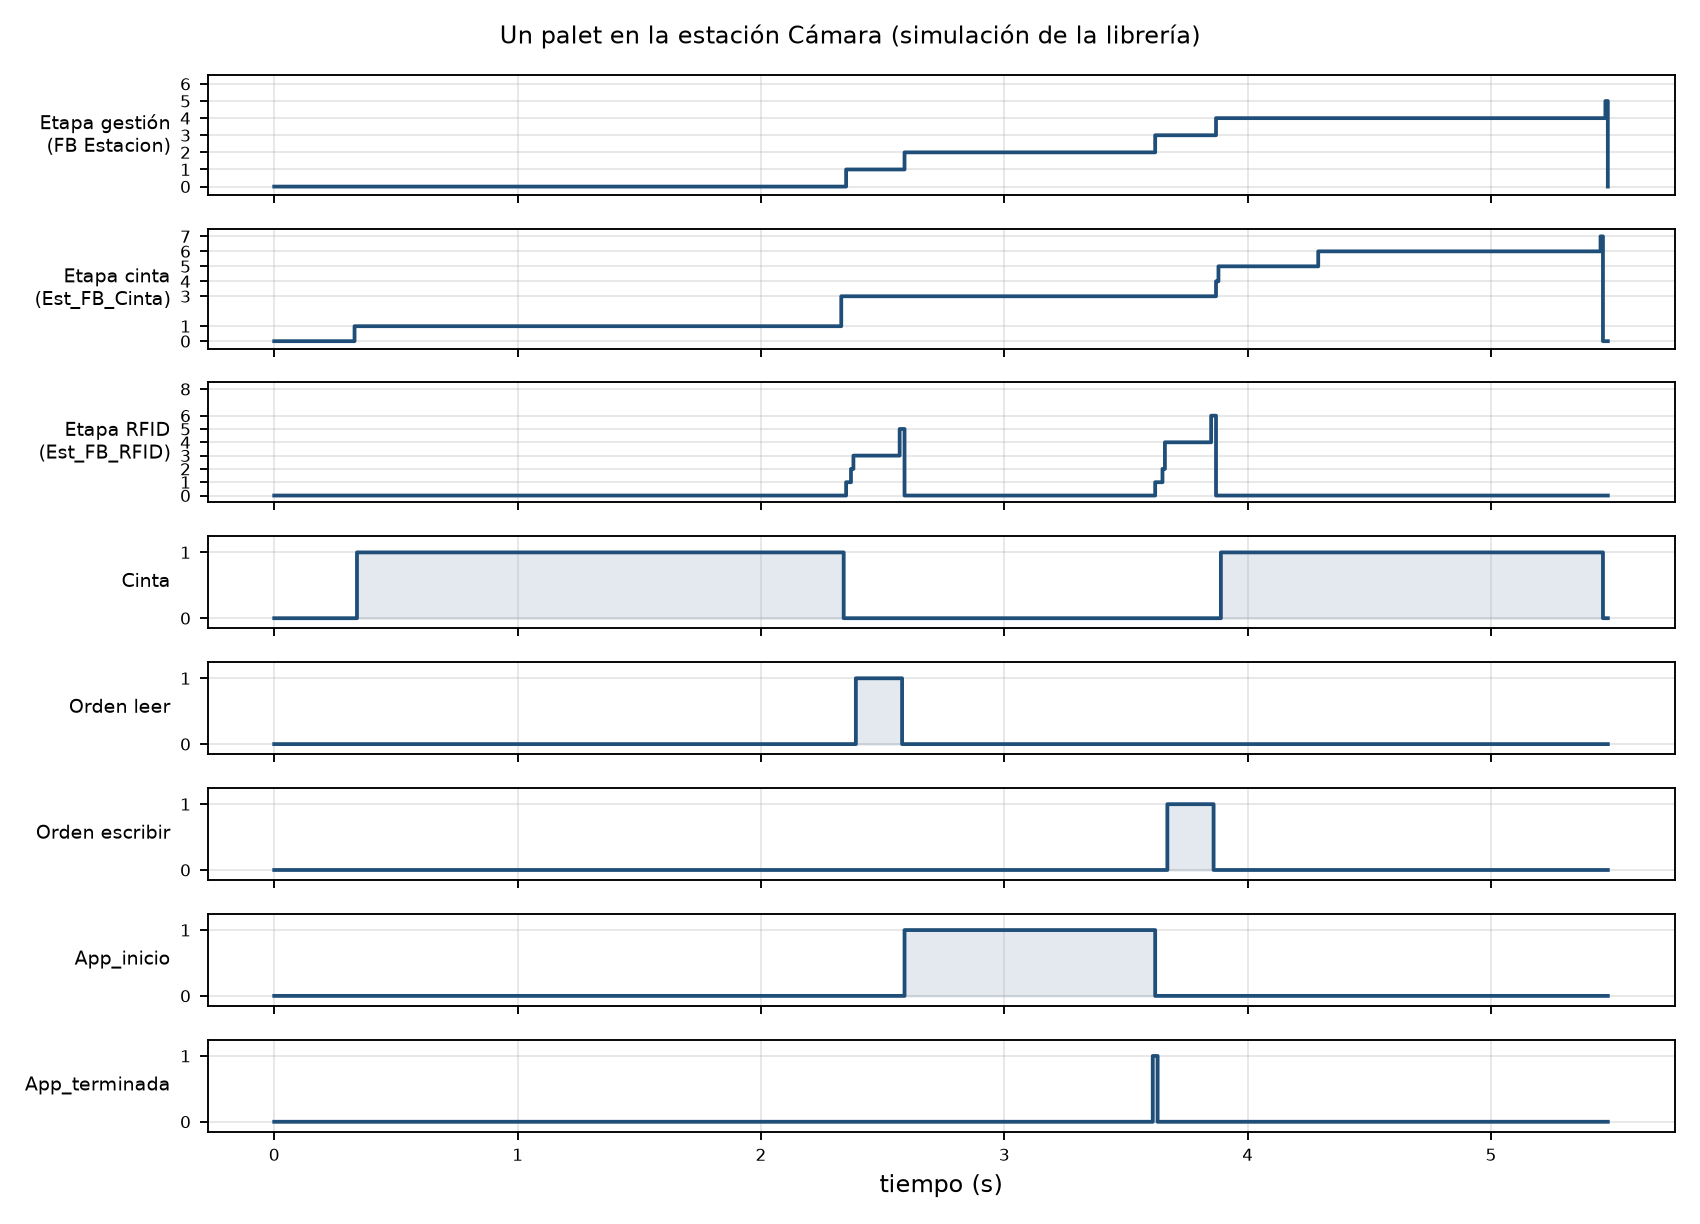
\includegraphics[width=\textwidth]{figuras/crono_ciclo_camara.png}
\caption{Un palet en la estación Cámara, simulación del código de la librería. De arriba abajo: etapa de la secuencia, etapa de la cinta, etapa del RFID, cinta en marcha, orden de leer, orden de escribir, \cod{App\_inicio} y \cod{App\_terminada}.}
\label{fig:crono}
\end{figure}

\section{Qué hay dentro del archivo de la librería}
El archivo \texttt{CPLabCore\_v\vlib.zal20} contiene dos cosas distintas, y conviene no confundirlas (la sección~\ref{sec:tipos-copias} explica la diferencia):

\begin{center}
\small
\begin{tabularx}{\textwidth}{>{\ttfamily\small}p{4.5cm}p{2.4cm}X}
\toprule
\textnormal{\textbf{Nombre}} & \textbf{Clase} & \textbf{Para qué sirve} \\
\midrule
\multicolumn{3}{l}{\sffamily\bfseries\color{azul} Tipos (con versión): lo que se usa tal cual} \\
Est\_FB\_Estacion & FB & La secuencia del palet; es lo único que llamas desde \cod{Main}. \\
Est\_FB\_Modo & FB & Botones, modos y emergencia. Lo llama \cod{Est\_FB\_Estacion}. \\
Est\_FB\_Cinta & FB & Cinta, stopper y recuento de palets. Lo llama \cod{Est\_FB\_Estacion}. \\
Est\_FB\_RFID & FB & Lector RFID. Lo llama \cod{Est\_FB\_Estacion}. \\
UDT\_Entradas\_Basico & UDT & Botonera y sensores de la cinta (módulo básico). \\
UDT\_Salidas\_Basico & UDT & Luces, cinta y stopper (módulo básico). \\
UDT\_Entradas\_Stopper & UDT & Sensores del módulo del stopper. \\
UDT\_Entradas\_RFID & UDT & Señales del lector RFID y los 28 bytes leídos. \\
UDT\_Salidas\_RFID & UDT & Órdenes al lector y los 28 bytes a escribir. \\
UDT\_Estado & UDT & Estado interno de la estación (modos, órdenes, errores). \\
\midrule
\multicolumn{3}{l}{\sffamily\bfseries\color{naranja!80!black} Copias maestras, carpeta \cod{Plantilla}: puntos de partida que copias y cambias} \\
Est\_FB\_App\_Plantilla & FB & Esqueleto vacío de aplicación, con el contrato ya hecho. \\
Main & OB & \cod{Main} de ejemplo con las dos llamadas cableadas. \\
DB\_Estacion & DB & Bloque de datos con las señales del contrato y la imagen. \\
Tabla de variables estándar & Tags & Los siete tags de E/S con su UDT y su dirección. \\
UDT\_Entradas\_APP, UDT\_Salidas\_APP & UDT & Ejemplo de E/S de aplicación (las de Out). \\
FB\_App\_Out, DB\_App\_out & FB, DB & La aplicación completa de la estación Out, como ejemplo. \\
\bottomrule
\end{tabularx}
\end{center}

\chapter{Cuatro ideas antes de seguir}\label{cap:conceptos}

Para usar la librería hacen falta cuatro ideas. Ninguna es difícil, pero conviene tenerlas claras: casi todos los errores de migración vienen de confundir alguna.

\section{Las entradas y salidas viajan en estructuras}
En un PLC Siemens, los sensores y actuadores llegan como bits en la \emph{imagen de proceso}: la entrada \cod{\%I1.0} es el primer bit del byte 1. Para no manejar bits sueltos, la librería agrupa los bits de cada módulo en un tipo de datos (UDT) con nombres: por ejemplo \cod{UDT\_Entradas\_Basico} tiene los miembros \cod{Boton\_marcha}, \cod{Boton\_paro}, etc. Después, \emph{una variable PLC} (un \emph{tag}) de ese tipo, situada en la dirección del módulo, hace que cada bit tenga su nombre.

\begin{idea}
El tag \cod{Entradas\_Basico} de tipo \cod{UDT\_Entradas\_Basico} en la dirección \cod{\%I1.0} \textbf{es} el byte de entradas 1 del PLC, visto con nombres. No hay que copiar nada: el nombre y el bit son la misma cosa.
\end{idea}

La librería usa cinco de estos tags comunes (los tienes en el apéndice~\ref{ap:direcciones}). Tu aplicación puede tener los suyos (\cod{UDT\_Entradas\_APP} y \cod{UDT\_Salidas\_APP}), que la librería no ve nunca.

\section{El palet lleva una memoria: el tag RFID}
Cada palet lleva un transpondedor (\emph{tag}) con 108 bytes de memoria. Es lo único que \textbf{viaja con el palet}: lo que una estación escribe en el tag, la siguiente lo lee. Por eso el tag es el idioma común de la línea.

El lector de cada estación (un SIMATIC RF210R conectado por IO-Link) no deja leer byte a byte. Funciona así:
\begin{itemize}
\item Se le da una \textbf{dirección de inicio} (un \emph{offset} en bytes dentro del tag) y una orden de leer o de escribir.
\item Lee o escribe siempre \textbf{un bloque de 28 bytes} a partir de esa dirección.
\item Termina cuando la señal \emph{proceso listo} baja y vuelve a subir, y la dirección que devuelve coincide con la que se pidió.
\end{itemize}

\begin{ojo}
Una escritura \textbf{siempre escribe los 28 bytes}, no solo los que tú quieres cambiar. Si escribes sin haber leído antes, los bytes que no tocas se quedan a cero y \emph{borras} lo que habían escrito las otras estaciones. Esta es la razón de ser de las máscaras (idea 3).
\end{ojo}

Hay un detalle más: el grupo acordó usar un único bloque de 28 bytes al principio del tag, a partir de la dirección que asigne el profesor (0 si el bloque es el primero). El reparto de esos 28 bytes está en el capítulo~\ref{cap:mapa}.

\section{La imagen del palet y las máscaras}
Para que tu aplicación no tenga que preocuparse del lector, la librería le entrega los datos del palet en una variable llamada \cod{Imagen\_palet}, un array de 28 bytes. Funciona como una fotocopia del bloque del tag con permisos:

\begin{figure}[ht]
\centering
\begin{tikzpicture}[x=1cm,y=1cm]
\node[hwcaja,minimum width=2.6cm,minimum height=1.5cm,font=\sffamily\small] (tag) at (0,0) {\textbf{Tag}\\[-1pt]\scriptsize 28 bytes del bloque};
\node[libcaja,minimum width=3.2cm,minimum height=1.5cm,font=\sffamily\small] (rf) at (4.4,0) {\cod{Est\_FB\_RFID}\\[-1pt]\scriptsize lee y escribe\\[-2pt]\scriptsize con las máscaras};
\node[caja,fill=white,minimum width=2.8cm,minimum height=1.5cm,font=\sffamily\small] (img) at (8.5,0) {\cod{Imagen\_palet}\\[-1pt]\scriptsize 28 bytes};
\node[appcaja,minimum width=2.6cm,minimum height=1.5cm,font=\sffamily\small] (app) at (12.3,0) {\textbf{Tu aplicación}};
\draw[flecha,<->] (tag) -- (rf);
\draw[flecha,<->] (rf) -- (img);
\draw[flecha,<->] (img) -- (app);
\node[etiqueta,above=2pt of $(tag.east)!0.5!(rf.west)$] {orden leer / escribir};
\node[etiqueta,below=14pt of rf,align=center] {\cod{Mascara\_lectura}: qué bytes llegan a la imagen\\\cod{Mascara\_escritura}: qué bytes vuelven al tag};
\end{tikzpicture}
\caption{El camino de los datos del palet.}
\end{figure}

\begin{itemize}
\item \textbf{Al leer}, a la imagen solo llegan los bytes que marca \cod{Mascara\_lectura}; el resto de la imagen queda a cero. Tu aplicación solo ve lo que necesita.
\item \textbf{Al escribir}, al tag solo van los bytes de la imagen que marca \cod{Mascara\_escritura}; los demás se devuelven al tag \emph{tal como se leyeron}. Tu aplicación no puede estropear los bytes de otras estaciones.
\end{itemize}

Cada máscara es un número de 32 bits en el que el bit $n$ corresponde al byte $n$ del bloque. En el capítulo~\ref{cap:mapa} se aprende a calcularlas.

\section{Tipos de la librería y copias maestras}\label{sec:tipos-copias}
Una librería global de TIA Portal guarda dos clases de cosas, que se usan de manera distinta:

\begin{description}[style=nextline,leftmargin=1.2cm]
\item[Tipos (\emph{Types}).] Tienen \textbf{versión}. Al arrastrarlos a tu proyecto quedan \emph{ligados} a la librería: no se editan en tu proyecto, y si sale una versión nueva se actualizan con un par de clics. Son las piezas que no debes tocar: los cuatro FB y los UDT comunes.
\item[Copias maestras (\emph{Master copies}).] Son copias normales, sin versión ni vínculo. Se arrastran a tu proyecto y son \textbf{tuyas}: las cambias como quieras. Son los puntos de partida: la plantilla de aplicación, el \cod{Main} de ejemplo, el bloque de datos y la tabla de variables.
\end{description}

\begin{idea}
Los tipos son \textbf{para usarlos}; las copias maestras son \textbf{para modificarlas}. Si algo tuyo tiene que cambiar, está en las copias maestras. Si algo de la librería tiene que cambiar, se pide un cambio en el tipo para todos.
\end{idea}

\section{Glosario}
\begin{center}
\small
\begin{tabularx}{\textwidth}{>{\bfseries}p{3.4cm}X}
\toprule
Palabra & Qué significa aquí \\
\midrule
Palet & La plataforma que lleva la pieza por la línea. Lleva un tag RFID. \\
Tag RFID & El transpondedor del palet; 108 bytes de memoria. La librería usa un bloque de 28. \\
Bloque & Los 28 bytes del tag que acordó el grupo (capítulo~\ref{cap:mapa}). \\
Imagen del palet & La copia en el PLC del bloque, con permisos (\cod{Imagen\_palet}). \\
Máscara & Número de 32 bits que dice qué bytes se leen o se escriben. \\
Contrato & Las ocho señales y la imagen que cumple tu aplicación para trabajar con la librería. \\
Aplicación & El bloque de función que es propio de cada estación. \\
FB / OB / DB & Bloque de función / bloque de organización (\cod{Main}) / bloque de datos. \\
UDT & Tipo de datos definido por el usuario (una estructura con nombres). \\
Tag (PLC) & Una variable del PLC con nombre y dirección. No confundir con el tag RFID. \\
Instancia & Cada llamada a un FB tiene su propia memoria, su bloque de datos de instancia. \\
Librería global & Archivo de TIA con tipos y copias maestras que se comparte entre proyectos. \\
\bottomrule
\end{tabularx}
\end{center}

\chapter{Los componentes por dentro}\label{cap:componentes}

Este capítulo explica, bloque por bloque, qué hace cada pieza de la librería, cómo se comporta y qué pines tiene. No necesitas aprendértelo: sirve para entender por qué la estación hace lo que hace y para saber dónde mirar cuando algo no va. Las tablas de pines están escritas para consultarlas.

\begin{consejo}
Todos los bloques siguen el mismo estilo: una máquina de estados con \texttt{CASE}, un número de etapa en una variable interna y las salidas puestas a su valor seguro al principio de cada ciclo. Si has leído uno, los demás se leen igual.
\end{consejo}

%=====================================================================
\section{\texttt{Est\_FB\_Estacion}: el director de orquesta}\label{sec:estacion}
Es el único bloque que llamas desde \cod{Main} (junto con tu aplicación). Dentro tiene una instancia de cada uno de los otros tres y los llama en orden. Hace tres cosas:

\begin{enumerate}
\item Calcula las \emph{condiciones} para que la estación pueda arrancar y para que la cinta pueda moverse.
\item Lleva la \textbf{secuencia del palet}, la máquina de estados de la figura~\ref{fig:fsm-gestion}.
\item Conecta las señales: pasa las entradas físicas a los otros bloques, y sus salidas a las luces, a la cinta, al lector y a tu aplicación.
\end{enumerate}

\subsection{La secuencia del palet}
\begin{figure}[ht]
\centering
\begin{tikzpicture}[x=1cm,y=1cm]
\node[estado] (s0) at (0,0) {0\\espera};
\node[estado] (s1) at (3.4,0) {1\\leer};
\node[estado,fill=naranja!15,draw=naranja] (s2) at (6.8,0) {2\\app};
\node[estado] (s3) at (10.2,0) {3\\escribir};
\node[estado] (s4) at (13.6,0) {4\\evacuar};
\node[estado] (s5) at (13.6,-2.8) {5\\fin};
\node[estado,fill=rojo!10,draw=rojo] (s6) at (6.8,3.0) {6\\fallo\\RFID};
\draw[flecha] (s0) -- node[etiqueta,above] {palet en posición} (s1);
\draw[flecha] (s1) -- node[etiqueta,above] {lectura ok} (s2);
\draw[flecha] (s2) -- node[etiqueta,above] {\cod{App\_terminada}} (s3);
\draw[flecha] (s3) -- node[etiqueta,above] {escritura ok} (s4);
\draw[flecha] (s4) -- node[etiqueta,right] {palet fuera} (s5);
\draw[flecha,rounded corners=4pt] (s5.south) -- ++(0,-0.9) -| node[etiqueta,pos=0.2,below] {siguiente palet} (s0.south);
\draw[flecha,rojo!80,rounded corners=4pt] (s1.north) |- node[etiqueta,pos=0.7,above,text=rojo] {error RFID} (s6.west);
\draw[flecha,rojo!80,rounded corners=4pt] (s3.north) |- node[etiqueta,pos=0.7,above,text=rojo] {error RFID} (s6.east);
\draw[flecha,rojo!80,rounded corners=4pt] (s6.north) -- ++(0,0.8) -| node[etiqueta,pos=0.25,above,text=rojo] {rearme: se evacúa sin procesar} (s4.north);
\node[etiqueta,align=left,anchor=north west,font=\sffamily\scriptsize] at (-0.8,-1.5) {Desde cualquier etapa:\\\textbf{Emergencia} $\rightarrow$ etapa 0};
\end{tikzpicture}
\caption{Secuencia del palet (\cod{Etapa\_gestion}). El camino rojo es el del fallo del lector.}
\label{fig:fsm-gestion}
\end{figure}

\begin{center}
\small
\begin{tabularx}{\textwidth}{>{\bfseries}p{1.2cm}p{3.3cm}X}
\toprule
Etapa & Qué activa & Para pasar a la siguiente \\
\midrule
0 & nada & ciclo auto o manual activo, palet en posición y sin emergencia. \\
1 & \cod{Orden\_leer} & \cod{Rfid\_lectura\_ok}. Si hay \cod{Rfid\_error}, a la 6. \\
2 & \cod{App\_inicio} & \cod{App\_terminada} (la sube tu aplicación). \\
3 & \cod{Orden\_escribir} & \cod{Rfid\_escritura\_ok}. Si hay \cod{Rfid\_error}, a la 6. \\
4 & \cod{Orden\_evacuar} (le dice a la cinta que suelte el palet) & \cod{Palet\_evacuado}. \\
5 & (fin del palet; en manual, termina el ciclo manual) & pasa a la 0 de inmediato. \\
6 & \cod{Rearme\_requerido\_gestion} (enciende la luz de rearme) & flanco del botón de rearme: evacúa el palet sin procesarlo (a la 4). \\
\bottomrule
\end{tabularx}
\end{center}

\subsection{Las condiciones de arranque}
La estación solo puede arrancar un ciclo cuando se cumplen a la vez estas condiciones iniciales (\cod{Estacion\_cond\_iniciales}):
\begin{itemize}
\item no hay emergencia;
\item el stopper no está bajado;
\item \textbf{tu aplicación está en reposo} (\cod{App\_en\_reposo}); es aquí donde tu aplicación puede impedir el arranque, por ejemplo si su mecanismo no está en la posición inicial;
\item no hay un error de RFID pendiente.
\end{itemize}
En modo automático eso basta para dar \cod{Marcha\_permitida} (se enciende la luz del botón de marcha). En modo manual, además, tiene que haber un palet en la estación. La cinta solo se mueve mientras haya un ciclo activo y sin emergencia (\cod{Cinta\_habilitada}).

\subsection{Luces y salidas que gobierna}
\begin{center}
\small
\begin{tabularx}{\textwidth}{>{\raggedright\arraybackslash\ttfamily\small}p{4.1cm}X}
\toprule
\textnormal{\textbf{Salida}} & \textbf{Cuándo se enciende} \\
\midrule
Led\_boton\_marcha & hay marcha permitida. \\
Led\_boton\_rearme & se pide rearme: tras emergencia, tras un fallo del RFID, o porque tu aplicación activa \cod{App\_rearme\_requerido}. \\
Led\_q1\_ciclo\_auto & el ciclo automático está activo. \\
Led\_q2\_emergencia & hay emergencia, o tu aplicación activa \cod{App\_alarma}. Si tu \cod{App\_alarma} parpadea, la luz parpadea. \\
Cinta\_dch & la cinta se mueve a la derecha (la decide \cod{Est\_FB\_Cinta}); se fuerza a apagado si \cod{Inhibir\_cinta} está activa. \\
Cinta\_izq, Cinta\_velocidad\_baja & siempre apagadas. \\
\bottomrule
\end{tabularx}
\end{center}

\subsection{Pines}
\begin{center}
\footnotesize
\begin{tabularx}{\textwidth}{>{\raggedright\arraybackslash\ttfamily}p{3.5cm}>{\raggedright\arraybackslash}p{1.1cm}>{\raggedright\arraybackslash\ttfamily}p{2.4cm}X}
\toprule
\textnormal{\textbf{Pin}} & \textbf{Dir.} & \textnormal{\textbf{Tipo}} & \textbf{Descripción} \\
\midrule
InBasico & entrada & UDT\_Entradas\_Basico & Botonera y sensores de la cinta (\cod{\%I1.0}). \\
InRFID & entrada & UDT\_Entradas\_RFID & Señales y datos del lector (\cod{\%I10.0}). \\
InStopper & entrada & UDT\_Entradas\_Stopper & Sensores del stopper (\cod{\%I42.0}). \\
Direccion\_lectura & entrada & Word & Dirección de inicio del bloque en el tag, para leer. Por defecto \cod{16\#0000}. \\
Direccion\_escritura & entrada & Word & Igual, para escribir. Por defecto \cod{16\#0000}. \\
Mascara\_lectura & entrada & DWord & Bytes del bloque que se leen a la imagen. Por defecto \cod{16\#0FFFFFFF} (todos). \\
Mascara\_escritura & entrada & DWord & Bytes de la imagen que se escriben. Por defecto \cod{16\#00000000} (ninguno). \\
App\_en\_reposo & entrada & Bool & Tu aplicación está lista para un palet. \\
App\_terminada & entrada & Bool & Tu aplicación ha terminado con este palet. \\
App\_alarma & entrada & Bool & Alarma de tu aplicación (parpadeo en la luz Q2). \\
App\_rearme\_requerido & entrada & Bool & Tu aplicación pide rearme (luz del botón). \\
Inhibir\_cinta & entrada & Bool & Si es verdadera, la cinta no se mueve. \\
\midrule
App\_inicio & salida & Bool & Orden de empezar a tu aplicación. \\
Emergencia & salida & Bool & Hay emergencia. \\
Rearme & salida & Bool & Pulso al pulsar rearme. \\
\midrule
OutBasico & in/out & UDT\_Salidas\_Basico & Luces, cinta y stopper (\cod{\%Q1.0}). \\
OutRFID & in/out & UDT\_Salidas\_RFID & Órdenes y datos al lector (\cod{\%Q10.0}). \\
Imagen\_palet & in/out & Array[0..27] of Byte & La imagen del palet (la comparte con tu aplicación). \\
\bottomrule
\end{tabularx}
\end{center}

\begin{ojo}
Los tres pines \cod{Direccion\_*} y los dos \cod{Mascara\_*} \textbf{son los que adaptas a tu estación}. Todo lo demás se cablea siempre igual en todas las estaciones.
\end{ojo}

%=====================================================================
\section{\texttt{Est\_FB\_Modo}: botones, modos y emergencia}\label{sec:modo}
Este bloque contiene tres máquinas de estados pequeñas e independientes entre sí (figura~\ref{fig:fsm-modo}).

\begin{figure}[ht]
\centering
\begin{tikzpicture}[x=1cm,y=1cm]
% Emergencia
\node[font=\sffamily\bfseries\small,anchor=east] at (-0.6,7.0) {Emergencia};
\node[estado] (n10) at (2.2,7.0) {10\\normal};
\node[estado,fill=rojo!10,draw=rojo] (n11) at (8.2,7.0) {11\\emerg.};
\draw[flecha] (n10.north east) to[bend left=28] node[etiqueta,above] {seta pulsada} (n11.north west);
\draw[flecha] (n11.south west) to[bend left=28] node[etiqueta,below] {rearme y seta suelta} (n10.south east);
% Modo
\node[font=\sffamily\bfseries\small,anchor=east] at (-0.6,4.0) {Modo};
\node[estado] (m20) at (2.2,4.0) {20\\manual};
\node[estado] (m21) at (8.2,4.0) {21\\auto};
\draw[flecha] (m20.north east) to[bend left=28] node[etiqueta,above] {selector en auto} (m21.north west);
\draw[flecha] (m21.south west) to[bend left=28] node[etiqueta,below] {selector en manual} (m20.south east);
% Ciclo
\node[font=\sffamily\bfseries\small,anchor=east] at (-0.6,0.0) {Ciclo};
\node[estado] (c30) at (2.2,0) {30\\reposo};
\node[estado,fill=verde!12,draw=verde] (c31) at (8.2,1.35) {31\\auto};
\node[estado,fill=verde!12,draw=verde] (c32) at (8.2,-1.35) {32\\manual};
\draw[flecha] (c30) to[bend left=14] node[etiqueta,above,sloped] {marcha (auto)} (c31);
\draw[flecha,rojo!70] (c31) to[bend left=14] (c30);
\draw[flecha] (c30) to[bend right=14] node[etiqueta,below,sloped] {marcha (manual)} (c32);
\draw[flecha,rojo!70] (c32) to[bend right=14] (c30);
\node[etiqueta,text=rojo,anchor=north west,align=left] at (3.6,-2.5) {flechas rojas: paro, emergencia, cambio de modo\\(y, en manual, ciclo manual acabado)};
\end{tikzpicture}
\caption{Las tres máquinas de \cod{Est\_FB\_Modo}.}
\label{fig:fsm-modo}
\end{figure}

\begin{description}[style=nextline,leftmargin=1.2cm]
\item[Emergencia.] Empieza en normal (etapa 10). Al pulsar la seta pasa a emergencia (11): activa \cod{Emergencia} y \cod{Rearme\_requerido}. Para volver a normal hace falta \textbf{soltar la seta y dar un flanco de rearme}. Con la seta pulsada, el rearme no basta.
\item[Modo.] Sigue al selector: manual (20) o automático (21). Cambiar de modo a mitad de ciclo lo detiene.
\item[Ciclo.] En reposo (30), si la estación puede arrancar (\cod{Condicion\_arranque\_auto} o \cod{\_manual}, según el modo) y no hay emergencia, activa \cod{Marcha\_permitida}. Con \cod{Marcha\_permitida}, un flanco del botón de marcha inicia el ciclo automático (31) o el manual (32). El ciclo termina con el paro, con una emergencia, con un cambio de modo o, en manual, cuando se ha terminado el palet (\cod{Ciclo\_manual\_acabado}).
\end{description}

\begin{center}
\footnotesize
\begin{tabularx}{\textwidth}{>{\raggedright\arraybackslash\ttfamily}p{3.7cm}>{\raggedright\arraybackslash}p{1.1cm}>{\raggedright\arraybackslash\ttfamily}p{1.0cm}X}
\toprule
\textnormal{\textbf{Pin}} & \textbf{Dir.} & \textnormal{\textbf{Tipo}} & \textbf{Descripción} \\
\midrule
Seta\_emergencia & entrada & Bool & Vale verdadero cuando \emph{hay} emergencia. \cod{Est\_FB\_Estacion} le pasa la señal ya invertida, porque la seta es de contacto cerrado. \\
Boton\_rearme, Boton\_marcha & entrada & Bool & Pulsadores. \\
Boton\_paro & entrada & Bool & Verdadero cuando se \emph{pulsa} el paro (también invertido, porque el paro es de contacto cerrado). \\
Selector\_automatico & entrada & Bool & Verdadero en automático. \\
Condicion\_arranque\_auto, Condicion\_arranque\_manual & entrada & Bool & Condiciones de arranque calculadas por \cod{Est\_FB\_Estacion}. \\
Ciclo\_manual\_acabado & entrada & Bool & Termina el ciclo manual. \\
Modo\_auto, Modo\_manual, Ciclo\_auto\_activo, Ciclo\_manual\_activo, Emergencia, Rearme\_requerido, Marcha\_permitida & in/out & Bool & Estados de salida; \cod{Est\_FB\_Estacion} los guarda en \cod{UDT\_Estado}. \\
\bottomrule
\end{tabularx}
\end{center}

%=====================================================================
\section{\texttt{Est\_FB\_Cinta}: la cinta y el stopper}\label{sec:cinta}
Controla la cinta y el stopper (el tope que frena el palet en la posición de trabajo) y lleva la cuenta de cuántos palets hay en la cinta, para saber si viene otro detrás. Su máquina de estados está en la figura~\ref{fig:fsm-cinta}.

\begin{figure}[ht]
\centering
\begin{tikzpicture}[x=1cm,y=1cm]
\node[estado] (c0) at (0,0) {0\\parada};
\node[estado] (c1) at (3.6,1.5) {1\\avance};
\node[estado,fill=verde!12,draw=verde] (c3) at (7.4,0) {3\\en tope};
\node[estado] (c4) at (11.8,0) {4\\liberar};
\node[estado] (c5) at (11.8,-3.0) {5\\sacar};
\node[estado] (c6) at (7.4,-3.0) {6\\salir};
\node[estado] (c7) at (3.6,-3.0) {7\\terminar};
\draw[flecha] (c0) -- node[etiqueta,above,sloped] {entra un palet} (c1);
\draw[flecha] (c1) -- node[etiqueta,above,sloped] {llega al tope} (c3);
\draw[flecha] (c0) -- node[etiqueta,above] {ya hay palet en el tope} (c3);
\draw[flecha] (c3) -- node[etiqueta,above] {\cod{Orden\_evacuar}} (c4);
\draw[flecha] (c4) -- node[etiqueta,right] {stopper abajo} (c5);
\draw[flecha] (c5) -- node[etiqueta,above,align=center] {0,4\,s o\\sensor dch.} (c6);
\draw[flecha] (c6) -- node[etiqueta,above] {palet salió} (c7);
\draw[flecha,rounded corners=4pt] (c7.west) -| node[etiqueta,pos=0.38,above] {\cod{Palet\_evacuado}} (c0.south);
\node[etiqueta,align=left,anchor=north west,font=\sffamily\scriptsize] at (-0.8,-4.6) {Desde cualquier etapa: \textbf{Emergencia} $\rightarrow$ etapa 0, cinta y stopper parados, contador a 0.\\Las etapas 1 y 6 tienen un límite de 10\,s: si el palet no llega o no sale, vuelven a una situación segura.};
\end{tikzpicture}
\caption{Máquina de estados de la cinta (\cod{Etapa\_cinta}).}
\label{fig:fsm-cinta}
\end{figure}

Además de las etapas, el bloque calcula dos señales que usa el director:
\begin{itemize}
\item \cod{Palet\_en\_posicion}: hay un palet parado en el tope, listo para trabajar (etapa 3).
\item \cod{Palet\_en\_estacion}: hay algún palet en algún punto de la estación (los sensores lo ven o el contador no es cero). La usa el modo manual.
\end{itemize}

\begin{ojo}
La etapa 2 (``asentar'') existe en el código pero ninguna transición llega a ella en esta versión. No es un error: es un resto de una versión anterior. Se puede ignorar. Y la etapa 4 avanza cuando \cod{Sensor\_stopper\_abajo} \emph{deja} de estar activo: conviene comprobar la polaridad de ese sensor en la maqueta real (apéndice~\ref{ap:abiertos}).
\end{ojo}

\begin{center}
\footnotesize
\begin{tabularx}{\textwidth}{>{\raggedright\arraybackslash\ttfamily}p{4.0cm}>{\raggedright\arraybackslash}p{1.1cm}X}
\toprule
\textnormal{\textbf{Pin}} & \textbf{Dir.} & \textbf{Descripción} \\
\midrule
Emergencia & entrada & Viene de \cod{Est\_FB\_Modo}. \\
Cinta\_habilitada & entrada & Ciclo activo y sin emergencia. \\
Orden\_evacuar & entrada & La aplicación ya terminó y el tag está escrito: soltar el palet. \\
Sensor\_palet\_izq, Sensor\_palet\_dch & entrada & Extremos de la cinta. \\
Sensor\_ind\_bien\_pos & entrada & Palet apoyado en el stopper (posición de trabajo). \\
Sensor\_stopper\_abajo & entrada & Confirmación del stopper. \\
Cinta\_dch, Bajar\_stopper & in/out & Actuadores. \\
Palet\_en\_posicion, Palet\_en\_estacion, Palet\_evacuado & in/out & Salidas de estado. \\
\bottomrule
\end{tabularx}
\end{center}

%=====================================================================
\section{\texttt{Est\_FB\_RFID}: el lector}\label{sec:rfid}
Es el bloque más delicado, porque el lector tiene un protocolo exigente (sección~\ref{cap:conceptos}) y porque aquí viven las máscaras. Se encarga de encender la antena, esperar a que detecte el tag, hacer una lectura o una escritura de 28 bytes y comprobar que ha acabado bien, con un límite de \textbf{5\,s} por operación.

\begin{figure}[ht]
\centering
\begin{tikzpicture}[x=1cm,y=1cm]
\node[estado] (r0) at (0,0) {0\\reposo};
\node[estado] (r1) at (3.1,0) {1\\energizar};
\node[estado] (r2) at (6.2,0) {2\\listo};
\node[estado,fill=azul!22] (r3) at (9.3,1.3) {3\\leer};
\node[estado,fill=azul!22] (r4) at (9.3,-1.3) {4\\escribir};
\node[estado,fill=verde!12,draw=verde] (r5) at (12.4,1.3) {5\\leído};
\node[estado,fill=verde!12,draw=verde] (r6) at (12.4,-1.3) {6\\escrito};
\node[estado,fill=rojo!10,draw=rojo] (r8) at (6.2,-3.1) {8\\error};
\draw[flecha] (r0) -- node[etiqueta,above] {orden} (r1);
\draw[flecha] (r1) -- node[etiqueta,above,align=center] {tag\\detectado} (r2);
\draw[flecha] (r2) -- (r3);
\draw[flecha] (r2) -- (r4);
\draw[flecha] (r3) -- (r5);
\draw[flecha] (r4) -- (r6);
\draw[flecha,rojo!80] (r1) -- (r8);
\draw[flecha,rojo!80] (r3) to[bend left=0] (r8);
\draw[flecha,rojo!80] (r4) -- (r8);
\draw[flechag,rounded corners=3pt] (r5.north) -- ++(0,0.8) -| node[etiqueta,pos=0.25,above] {orden leer baja} (r0.north);
\draw[flechag,rounded corners=3pt] (r6.south) -- ++(0,-0.9) -| (r0.south);
\node[etiqueta,align=left,anchor=north west,font=\sffamily\scriptsize] at (-0.8,-3.0) {Error: lector con error o 5\,s sin\\respuesta. Sale al bajar las órdenes.\\Emergencia $\rightarrow$ etapa 0 y antena apagada.};
\end{tikzpicture}
\caption{Máquina de estados del lector.}
\label{fig:fsm-rfid}
\end{figure}

\subsection{Cómo lee}
\begin{enumerate}
\item \textbf{Energizar (1).} Enciende la antena y espera: antena no apagada, tag detectado, lector listo.
\item \textbf{Listo (2).} Espera la orden. Si es leer, va a la etapa 3.
\item \textbf{Leer (3).} Escribe la dirección de inicio (\cod{Direccion\_lectura}) y activa \cod{Tag\_leer}. El lector baja \emph{proceso listo} (ha empezado, y el bloque lo anota en \cod{Rfid\_ocupado}), lee, y vuelve a subirlo. Solo cuando \emph{listo} ha bajado y vuelto a subir, \cod{Tag\_datos\_leidos} está activo y la dirección devuelta coincide con la pedida, el dato vale. Entonces:
  \begin{itemize}
  \item copia los 28 bytes recibidos en la copia interna \cod{Imagen\_leida};
  \item rellena \cod{Imagen\_palet} con los bytes cuyo bit está en \cod{Mascara\_lectura}, y \textbf{pone a cero} los demás;
  \item pasa a «leído» (5), que deja \cod{Rfid\_lectura\_ok} activo hasta que la orden de leer baje.
  \end{itemize}
\end{enumerate}

\subsection{Cómo escribe}
Es la operación simétrica. En la etapa 4, a cada ciclo, \textbf{construye el bloque que va al tag}: para cada byte $i$ de 0 a 27,
\begin{itemize}
\item si el bit $i$ de \cod{Mascara\_escritura} está a 1, usa el byte $i$ de \cod{Imagen\_palet} (el que dejó tu aplicación);
\item si está a 0, usa el byte $i$ de \cod{Imagen\_leida}, es decir, \textbf{el mismo valor que tenía al leer}.
\end{itemize}
Con eso, la escritura de 28 bytes es inofensiva para los bytes de las demás estaciones. Cuando el lector confirma (con la dirección \cod{Direccion\_escritura}), pasa a «escrito» (6).

\begin{peligro}
Esto solo funciona si \textbf{la misma estación ha leído antes} el palet con la misma dirección. Por eso la secuencia siempre es «leer, trabajar, escribir» en el mismo palet. Si algún día una estación escribe sin haber leído, los bytes ajenos se escribirían con lo último que se leyó, que podría ser de otro palet. La librería no permite esta situación en su secuencia normal, pero tenlo presente si escribes cosas especiales.
\end{peligro}

\subsection{Errores}
Si \cod{Tag\_error} se activa, o la operación tarda más de 5\,s en alguna de las etapas 1, 3 o 4, el bloque pasa al estado de error (8): activa \cod{Rfid\_error}, guarda el código que da el lector en \cod{Rfid\_codigo\_error}, apaga la antena y espera a que las órdenes bajen para volver a reposo. \cod{Est\_FB\_Estacion} reacciona con la etapa 6 de la secuencia.

\begin{center}
\footnotesize
\begin{tabularx}{\textwidth}{>{\raggedright\arraybackslash\ttfamily}p{4.4cm}>{\raggedright\arraybackslash}p{1.1cm}X}
\toprule
\textnormal{\textbf{Pin}} & \textbf{Dir.} & \textbf{Descripción} \\
\midrule
Orden\_leer, Orden\_escribir & entrada & Órdenes de la secuencia. Una cada vez. \\
Emergencia & entrada & Aborta la operación y apaga la antena. \\
Direccion\_lectura, Direccion\_escritura & entrada & Dirección de inicio del bloque, en bytes (Word). \\
Mascara\_lectura, Mascara\_escritura & entrada & Bytes que se leen o escriben (DWord, un bit por byte). \\
Tag\_datos\_escritos, Tag\_datos\_leidos, Tag\_antena\_apagada, Tag\_detectado, Tag\_error, Tag\_proceso\_listo & entrada & Señales del lector (\cod{UDT\_Entradas\_RFID}). \\
Tag\_codigo\_error, Tag\_direccion\_confirmada, Tag\_datos\_leidos\_escritos & entrada & Código de error, dirección que confirma el lector y los 28 bytes leídos. \\
Tag\_escribir, Tag\_leer, Tag\_antena\_apagar, Tag\_direccion\_leer\_escribir, Tag\_datos\_a\_escribir & in/out & Órdenes, dirección y los 28 bytes que se escriben. \\
Rfid\_lectura\_ok, Rfid\_escritura\_ok, Rfid\_error, Rfid\_codigo\_error & in/out & Resultado de la operación. \\
Imagen & in/out & La imagen del palet (28 bytes). \\
\bottomrule
\end{tabularx}
\end{center}

%=====================================================================
\section{Los tipos de datos (UDT)}\label{sec:udts}
Los seis UDT de la librería agrupan, con nombre, los bits de cada módulo. No hay que aprenderlos de memoria (el apéndice~\ref{ap:direcciones} los lista con su dirección), pero sí saber para qué sirve cada uno:

\begin{center}
\small
\begin{tabularx}{\textwidth}{>{\raggedright\arraybackslash\ttfamily\small}p{4.2cm}p{2.4cm}X}
\toprule
\textnormal{\textbf{UDT}} & \textbf{Tag y dirección} & \textbf{Qué contiene} \\
\midrule
UDT\_Entradas\_Basico & \cod{Entradas\_Basico} \cod{\%I1.0} & Botones de marcha, paro y rearme, selector, seta, sensores de palet en la cinta. \\
UDT\_Salidas\_Basico & \cod{Salidas\_Basico} \cod{\%Q1.0} & Luces del panel, cinta (derecha, izquierda, lenta), stopper. \\
UDT\_Entradas\_Stopper & \cod{Entradas\_Stopper} \cod{\%I42.0} & Cuatro sensores inductivos y el sensor «stopper abajo». \\
UDT\_Entradas\_RFID & \cod{Entradas\_RFID} \cod{\%I10.0} & Estado del lector, código de error, dirección, 28 bytes leídos. \\
UDT\_Salidas\_RFID & \cod{Salidas\_RFID} \cod{\%Q10.0} & Órdenes de leer y escribir, antena, dirección, 28 bytes a escribir. \\
UDT\_Estado & (interno) & Estado de la estación: modos, órdenes, errores. Vive dentro de \cod{Est\_FB\_Estacion}. No se toca. \\
\bottomrule
\end{tabularx}
\end{center}

Los miembros llamados \cod{Reservado\_...} y \cod{Tag\_reservado\_...} ocupan los bits que el módulo tiene pero la librería no usa. Están ahí para que los miembros siguientes caigan en el byte y el bit correctos. \textbf{No los borres ni cambies el orden de los miembros}: cada miembro tiene que estar exactamente en el bit que le corresponde del módulo físico.

\chapter{El contrato con tu aplicación}\label{cap:contrato}

Este es el capítulo más importante para quien tenga que escribir o adaptar una aplicación. El contrato es pequeño a propósito: ocho señales y una imagen. Si tu aplicación lo cumple, funciona con la librería; si no, la estación se queda esperando.

\section{Las señales}
Se miran siempre desde \textbf{tu aplicación}. Tienes cuatro cosas que \emph{recibes} y cinco que \emph{entregas}:

\begin{center}
\small
\begin{tabularx}{\textwidth}{>{\ttfamily\small}p{3.7cm}>{\raggedright\arraybackslash}p{1.3cm}p{1.1cm}X}
\toprule
\textnormal{\textbf{Señal}} & \textbf{Sentido} & \textbf{Tipo} & \textbf{Qué significa} \\
\midrule
App\_inicio & recibes & Bool & «Empieza»: hay un palet en posición y su tag ya está leído en la imagen. Se mantiene activa hasta que entregues \cod{App\_terminada}. \\
Emergencia & recibes & Bool & Hay emergencia. Detén tus actuadores y vuelve a reposo. \\
Rearme & recibes & Bool & Pulso: se ha pulsado el botón de rearme. \\
Imagen\_palet & recibes y devuelves & Array[0..27] of Byte & Los datos del palet. Lees de aquí y escribes aquí (sección~\ref{sec:imagen}). \\
\midrule
App\_en\_reposo & entregas & Bool & «Estoy lista para recibir un palet.» Sin ella, la estación no arranca. \\
App\_terminada & entregas & Bool & «He acabado con este palet y he dejado el resultado en la imagen.» \\
App\_alarma & entregas & Bool & Opcional. Hace parpadear la luz Q2. Para avisar de un problema de tu aplicación. \\
App\_rearme\_requerido & entregas & Bool & Opcional. Enciende la luz del botón de rearme: «necesito que alguien pulse rearme». \\
Inhibir\_cinta & entregas & Bool & Si la activas, la cinta no se mueve. Úsala cuando tu mecanismo estorbe (p.\,ej., la garra de Out con el eje Z abajo). \\
\bottomrule
\end{tabularx}
\end{center}

\section{La conversación, en el tiempo}
La figura~\ref{fig:cronograma-contrato} muestra una conversación normal entre la librería (arriba) y tu aplicación (abajo). Léela de izquierda a derecha.

\begin{figure}[ht]
\centering
\begin{tikzpicture}[x=1cm,y=1cm]
\def\h{0.55}
% ejes
\foreach \i/\n/\c in {0/{\cod{Palet\_en\_posicion}}/azul,1/{\cod{Orden\_leer} / \cod{Rfid\_lectura\_ok}}/azul,2/{\cod{App\_en\_reposo}}/naranja,3/{\cod{App\_inicio}}/azul,4/{\cod{App\_terminada}}/naranja,5/{\cod{Orden\_escribir}}/azul,6/{\cod{Orden\_evacuar}}/azul}{
  \node[font=\sffamily\scriptsize,anchor=east] at (-0.2,-\i*1.0+0.28) {\n};
  \draw[gris!50] (0,-\i*1.0) -- (12.4,-\i*1.0);}
% palet en posicion: sube en 1, baja en 9.6
\draw[azul,very thick] (0,0) -- (1,0) -- (1,\h) -- (9.4,\h) -- (9.4,0) -- (12.4,0);
% leer
\draw[azul,very thick] (0,-1) -- (1.2,-1) -- (1.2,-1+\h) -- (2.6,-1+\h) -- (2.6,-1) -- (12.4,-1);
% reposo (app)
\draw[naranja,very thick] (0,-2+\h) -- (2.9,-2+\h) -- (2.9,-2) -- (7.2,-2) -- (7.2,-2+\h) -- (12.4,-2+\h);
% inicio
\draw[azul,very thick] (0,-3) -- (2.9,-3) -- (2.9,-3+\h) -- (7.0,-3+\h) -- (7.0,-3) -- (12.4,-3);
% terminada
\draw[naranja,very thick] (0,-4) -- (6.5,-4) -- (6.5,-4+\h) -- (7.2,-4+\h) -- (7.2,-4) -- (12.4,-4);
% escribir
\draw[azul,very thick] (0,-5) -- (7.0,-5) -- (7.0,-5+\h) -- (8.6,-5+\h) -- (8.6,-5) -- (12.4,-5);
% evacuar
\draw[azul,very thick] (0,-6) -- (8.7,-6) -- (8.7,-6+\h) -- (9.4,-6+\h) -- (9.4,-6) -- (12.4,-6);
% marcas
\draw[dashed,gris] (2.9,0.8) -- (2.9,-6.3);
\draw[dashed,gris] (7.0,0.8) -- (7.0,-6.3);
\node[etiqueta,font=\sffamily\scriptsize\bfseries] at (2.9,0.95) {1};
\node[etiqueta,font=\sffamily\scriptsize\bfseries] at (7.0,0.95) {2};
\node[etiqueta,font=\sffamily\scriptsize,align=left,anchor=north west] at (0,-6.55) {\textbf{1} La librería ha leído el tag y sube \cod{App\_inicio}; tu aplicación deja de estar en reposo.\\\textbf{2} Tu aplicación acaba y sube \cod{App\_terminada}; la librería baja \cod{App\_inicio} y empieza a escribir el tag. Solo entonces tu aplicación baja \cod{App\_terminada} y vuelve a reposo.};
\end{tikzpicture}
\caption{Una conversación normal entre la librería (azul) y tu aplicación (naranja). Las líneas altas son «verdadero».}
\label{fig:cronograma-contrato}
\end{figure}

\section{Las reglas del contrato}\label{sec:reglas}
Son siete. Si las cumples, tu aplicación funciona con la librería.

\begin{enumerate}[leftmargin=1.2cm,label=\textbf{R\arabic*.}]
\item \textbf{Declara cuándo estás en reposo.} \cod{App\_en\_reposo} debe ser verdadera cuando tu mecanismo está en su posición inicial y puede recibir un palet. Es la forma de impedir que la estación arranque con tu mecanismo a medias.
\item \textbf{Empieza solo con \cod{App\_inicio}, y solo si estás en reposo.} Mientras trabajas, \cod{App\_en\_reposo} debe ser falsa.
\item \textbf{Termina con \cod{App\_terminada} y mantenla.} Debe seguir verdadera \emph{hasta que \cod{App\_inicio} baje}. Es la forma que se ha probado y no depende de nada más. Un pulso de un solo ciclo puede funcionar con el orden de llamadas recomendado, pero es frágil: si alguna vez cambia el orden de las llamadas en \cod{Main}, tu aplicación podría volver a reposo viendo \cod{App\_inicio} todavía activa y empezar otra vez con el mismo palet.
\item \textbf{Deja el resultado en la imagen antes de terminar.} Todo lo que quieras escribir en el tag tiene que estar ya en \cod{Imagen\_palet} cuando subas \cod{App\_terminada}. La librería escribe el tag justo después.
\item \textbf{Toca solo tus bytes.} Escribe en \cod{Imagen\_palet} solo los bytes que están en tu \cod{Mascara\_escritura}, y lee solo los que están en tu \cod{Mascara\_lectura}. Lo demás es de otras estaciones (capítulo~\ref{cap:mapa}).
\item \textbf{Obedece la emergencia.} Con \cod{Emergencia} verdadera, apaga todos tus actuadores peligrosos y vuelve a tu estado inicial. Tu aplicación puede quedar fuera de reposo (por ejemplo, con una pieza en la garra); en ese caso mantén \cod{App\_en\_reposo} falsa hasta haberte recolocado, y si lo necesitas pide el rearme con \cod{App\_rearme\_requerido}.
\item \textbf{No esperes cosas que la librería no hace.} No hay límite de tiempo para tu aplicación: si nunca subes \cod{App\_terminada}, la estación esperará para siempre. Si tu mecanismo puede atascarse, pon tu propio temporizador y reacciona con \cod{App\_alarma}.
\end{enumerate}

\begin{ojo}
La regla R3 es la que más se pasa por alto, porque una aplicación que sube \cod{App\_terminada} un instante parece funcionar. Haz lo que hace la plantilla: pasar a una etapa «fin» y no salir de ella hasta que \cod{App\_inicio} baje.
\end{ojo}

\section{La imagen del palet}\label{sec:imagen}
\cod{Imagen\_palet} es un array de 28 bytes, índices de 0 a 27, que corresponden a los bytes 0 a 27 del bloque del tag. Es muy cómodo usarla con constantes con nombre:

\begin{lstlisting}[caption={Cómo se usa la imagen en una aplicación (extracto de la plantilla).}]
VAR CONSTANT
    IDX_CALIDAD  : Int  := 5;     // byte 5 del bloque: calidad global
    IDX_COMPLETADAS : Int := 4;   // byte 4: estaciones completadas
    BIT_PRESS    : Byte := 16#04; // bit 2: Press
END_VAR

// leer:
IF #Imagen_palet[#IDX_CALIDAD] = 1 THEN ... END_IF;
// escribir, sin tocar los demas bits del byte:
#Imagen_palet[#IDX_COMPLETADAS] := #Imagen_palet[#IDX_COMPLETADAS] OR #BIT_PRESS;
\end{lstlisting}

Dos observaciones importantes:
\begin{itemize}
\item Los bytes que no estén en \cod{Mascara\_lectura} te llegan \textbf{a cero}, aunque en el tag haya otra cosa. Esto es una protección: tu aplicación no depende de bytes que no son suyos.
\item Un byte tuyo para escribir tiene que estar \textbf{también en \cod{Mascara\_lectura}}, salvo que quieras sobrescribirlo siempre con un valor fijo. Si no, la imagen lo tiene a cero y escribirías cero encima del valor del tag. Este es el error más frecuente con las máscaras; el capítulo~\ref{cap:mapa} da la regla exacta.
\end{itemize}

\section{El orden de las llamadas en \texttt{Main}}
En \cod{Main}, primero va \cod{Est\_FB\_Estacion} y después tu aplicación. Las señales que van de la librería a tu aplicación (\cod{App\_inicio}, \cod{Emergencia}, \cod{Rearme}) llegan en el \textbf{mismo} ciclo de scan. Las que vuelven (\cod{App\_en\_reposo}, \cod{App\_terminada}, \dots) llegan a la librería un ciclo después, lo que no importa porque son niveles que se mantienen. \cod{Rearme} es la única que dura un solo ciclo, y tu aplicación la recibe en ese ciclo.

\section{Tu aplicación en una página: la plantilla}
La copia maestra \cod{Est\_FB\_App\_Plantilla} (listado completo en el apéndice~\ref{ap:listados}) es el esqueleto que debes copiar. Su máquina de estados es esta:

\begin{figure}[ht]
\centering
\begin{tikzpicture}[x=1cm,y=1cm]
\node[estado,fill=naranja!10,draw=naranja] (a0) at (0,0) {0\\reposo};
\node[estado,fill=naranja!10,draw=naranja] (a1) at (4.2,0) {10\\trabajo};
\node[estado,fill=naranja!10,draw=naranja] (a2) at (8.4,0) {20\\fin};
\draw[flecha] (a0) -- node[etiqueta,above] {\cod{App\_inicio} y en reposo} (a1);
\draw[flecha] (a1) -- node[etiqueta,above] {tu secuencia termina} (a2);
\draw[flecha,rounded corners=3pt] (a2.south) -- ++(0,-1.0) -| node[etiqueta,pos=0.25,below] {\cod{App\_inicio} baja} (a0.south);
\node[etiqueta,align=left,font=\sffamily\scriptsize,anchor=north west] at (-0.6,-2.2) {En reposo: \cod{App\_en\_reposo} verdadera.\ \ En fin: \cod{App\_terminada} verdadera.\\Con \cod{Emergencia}: vuelve a 0 y apaga tus actuadores.};
\end{tikzpicture}
\caption{La plantilla de aplicación: tres estados. Tu secuencia real se escribe dentro de «trabajo», que puedes ampliar con todas las etapas que necesites.}
\end{figure}

Para adaptarla solo tienes que:
\begin{enumerate}
\item sustituir el contenido del estado 10 por la secuencia de tu estación (puede tener tantas etapas como quieras, mientras acabe pasando al estado de fin);
\item cambiar la condición de \cod{App\_en\_reposo} en el estado 0 por la tuya;
\item añadir tus entradas y salidas físicas al bloque, y cablearlas en \cod{Main};
\item declarar tus constantes \cod{IDX\_*} y usar la imagen.
\end{enumerate}
El capítulo~\ref{cap:migracion} lo hace paso a paso, con ejemplos completos para Press, BackCover y Cámara.

\section{Cómo comprobar que tu aplicación cumple el contrato}
Antes de probar con la estación completa, merece la pena comprobar estas cinco cosas, que se ven directamente en el \emph{observar y modificar} de TIA (o en la tabla de observación):
\begin{enumerate}
\item Con la estación parada, \cod{App\_en\_reposo} está en verdadero.
\item Al forzar \cod{App\_inicio} a verdadero, \cod{App\_en\_reposo} baja y tu mecanismo empieza.
\item Al acabar, \cod{App\_terminada} sube, y \textbf{se queda} mientras \cod{App\_inicio} esté activa.
\item Al bajar \cod{App\_inicio}, \cod{App\_terminada} baja y \cod{App\_en\_reposo} vuelve a subir.
\item Al activar \cod{Emergencia} en cualquier momento, tus actuadores se apagan y la aplicación vuelve a reposo (o declara que necesita rearme).
\end{enumerate}

\chapter{El mapa del tag y las máscaras}\label{cap:mapa}

Este capítulo es el pegamento entre las estaciones. La librería solo transporta bytes; aquí se explica qué significa cada uno, cómo elige cada estación los suyos, y cómo se calculan las máscaras.

\section{El bloque de 28 bytes}
El grupo acordó (hoja de cálculo \texttt{Mapa\_RFID\_CPLab.xlsx}) usar un único bloque de 28 bytes en el tag. Los bytes 0 a 19 son del grupo; los bytes 20 a 27 están reservados para compartir con los otros grupos de la CP-Lab. La figura~\ref{fig:bloque} los muestra con un color por quién los usa.

\begin{figure}[ht]
\centering
\begin{tikzpicture}[x=0.585cm,y=1cm]
\fill[gris!35] (0,-0.00) rectangle (1,0.80);\draw[gray!70] (0,-0.00) rectangle (1,0.80);
\node[font=\scriptsize\bfseries] at (0.5,0.40) {0};
\fill[gris!35] (1,-0.00) rectangle (2,0.80);\draw[gray!70] (1,-0.00) rectangle (2,0.80);
\node[font=\scriptsize\bfseries] at (1.5,0.40) {1};
\fill[gris!35] (2,-0.00) rectangle (3,0.80);\draw[gray!70] (2,-0.00) rectangle (3,0.80);
\node[font=\scriptsize\bfseries] at (2.5,0.40) {2};
\fill[gris!35] (3,-0.00) rectangle (4,0.80);\draw[gray!70] (3,-0.00) rectangle (4,0.80);
\node[font=\scriptsize\bfseries] at (3.5,0.40) {3};
\fill[gris!35] (4,-0.00) rectangle (5,0.80);\draw[gray!70] (4,-0.00) rectangle (5,0.80);
\node[font=\scriptsize\bfseries] at (4.5,0.40) {4};
\fill[gris!35] (5,-0.00) rectangle (6,0.80);\draw[gray!70] (5,-0.00) rectangle (6,0.80);
\node[font=\scriptsize\bfseries] at (5.5,0.40) {5};
\fill[gris!35] (6,-0.00) rectangle (7,0.80);\draw[gray!70] (6,-0.00) rectangle (7,0.80);
\node[font=\scriptsize\bfseries] at (6.5,0.40) {6};
\fill[gris!35] (7,-0.00) rectangle (8,0.80);\draw[gray!70] (7,-0.00) rectangle (8,0.80);
\node[font=\scriptsize\bfseries] at (7.5,0.40) {7};
\fill[cam!35] (8,-0.00) rectangle (9,0.80);\draw[gray!70] (8,-0.00) rectangle (9,0.80);
\node[font=\scriptsize\bfseries] at (8.5,0.40) {8};
\fill[cam!35] (9,-0.00) rectangle (10,0.80);\draw[gray!70] (9,-0.00) rectangle (10,0.80);
\node[font=\scriptsize\bfseries] at (9.5,0.40) {9};
\fill[cam!35] (10,-0.00) rectangle (11,0.80);\draw[gray!70] (10,-0.00) rectangle (11,0.80);
\node[font=\scriptsize\bfseries] at (10.5,0.40) {10};
\fill[cam!35] (11,-0.00) rectangle (12,0.80);\draw[gray!70] (11,-0.00) rectangle (12,0.80);
\node[font=\scriptsize\bfseries] at (11.5,0.40) {11};
\fill[back!35] (12,-0.00) rectangle (13,0.80);\draw[gray!70] (12,-0.00) rectangle (13,0.80);
\node[font=\scriptsize\bfseries] at (12.5,0.40) {12};
\fill[press!35] (13,-0.00) rectangle (14,0.80);\draw[gray!70] (13,-0.00) rectangle (14,0.80);
\node[font=\scriptsize\bfseries] at (13.5,0.40) {13};
\fill[press!35] (0,-1.55) rectangle (1,-0.75);\draw[gray!70] (0,-1.55) rectangle (1,-0.75);
\node[font=\scriptsize\bfseries] at (0.5,-1.15) {14};
\fill[press!35] (1,-1.55) rectangle (2,-0.75);\draw[gray!70] (1,-1.55) rectangle (2,-0.75);
\node[font=\scriptsize\bfseries] at (1.5,-1.15) {15};
\fill[press!35] (2,-1.55) rectangle (3,-0.75);\draw[gray!70] (2,-1.55) rectangle (3,-0.75);
\node[font=\scriptsize\bfseries] at (2.5,-1.15) {16};
\fill[out!35] (3,-1.55) rectangle (4,-0.75);\draw[gray!70] (3,-1.55) rectangle (4,-0.75);
\node[font=\scriptsize\bfseries] at (3.5,-1.15) {17};
\fill[out!35] (4,-1.55) rectangle (5,-0.75);\draw[gray!70] (4,-1.55) rectangle (5,-0.75);
\node[font=\scriptsize\bfseries] at (4.5,-1.15) {18};
\fill[gris!35] (5,-1.55) rectangle (6,-0.75);\draw[gray!70] (5,-1.55) rectangle (6,-0.75);
\node[font=\scriptsize\bfseries] at (5.5,-1.15) {19};
\fill[comp!35] (6,-1.55) rectangle (7,-0.75);\draw[gray!70] (6,-1.55) rectangle (7,-0.75);
\node[font=\scriptsize\bfseries] at (6.5,-1.15) {20};
\fill[comp!35] (7,-1.55) rectangle (8,-0.75);\draw[gray!70] (7,-1.55) rectangle (8,-0.75);
\node[font=\scriptsize\bfseries] at (7.5,-1.15) {21};
\fill[comp!35] (8,-1.55) rectangle (9,-0.75);\draw[gray!70] (8,-1.55) rectangle (9,-0.75);
\node[font=\scriptsize\bfseries] at (8.5,-1.15) {22};
\fill[comp!35] (9,-1.55) rectangle (10,-0.75);\draw[gray!70] (9,-1.55) rectangle (10,-0.75);
\node[font=\scriptsize\bfseries] at (9.5,-1.15) {23};
\fill[comp!35] (10,-1.55) rectangle (11,-0.75);\draw[gray!70] (10,-1.55) rectangle (11,-0.75);
\node[font=\scriptsize\bfseries] at (10.5,-1.15) {24};
\fill[comp!35] (11,-1.55) rectangle (12,-0.75);\draw[gray!70] (11,-1.55) rectangle (12,-0.75);
\node[font=\scriptsize\bfseries] at (11.5,-1.15) {25};
\fill[comp!35] (12,-1.55) rectangle (13,-0.75);\draw[gray!70] (12,-1.55) rectangle (13,-0.75);
\node[font=\scriptsize\bfseries] at (12.5,-1.15) {26};
\fill[comp!35] (13,-1.55) rectangle (14,-0.75);\draw[gray!70] (13,-1.55) rectangle (14,-0.75);
\node[font=\scriptsize\bfseries] at (13.5,-1.15) {27};
\end{tikzpicture}
\\[6pt]
\small
\tikz\fill[gris!35] (0,0) rectangle (0.35,0.25);\ General\quad
\tikz\fill[cam!35] (0,0) rectangle (0.35,0.25);\ Cámara\quad
\tikz\fill[back!35] (0,0) rectangle (0.35,0.25);\ BackCover\quad
\tikz\fill[press!35] (0,0) rectangle (0.35,0.25);\ Press\quad
\tikz\fill[out!35] (0,0) rectangle (0.35,0.25);\ Out\quad
\tikz\fill[comp!35] (0,0) rectangle (0.35,0.25);\ Compartido (otros grupos)
\caption{Los 28 bytes del bloque, byte a byte (0 a 13 arriba, 14 a 27 abajo).}
\label{fig:bloque}
\end{figure}

\begin{idea}
El tag es un \textbf{tablón compartido}. Cada byte tiene un dueño que lo escribe, y varios que lo leen. Que un byte tenga un solo dueño es lo que impide que las estaciones se pisen. La excepción son los bytes de «banderas» (el byte 4, que cada estación completa con su bit); para esos hay una regla especial (sección~\ref{sec:reglas-oro}).
\end{idea}

\section{El mapa completo}
La tabla siguiente es el contenido de la hoja «Mapa RFID» del Excel del grupo. Las filas están coloreadas por estación. \textbf{Si alguna vez la tabla de este documento y el Excel difieren, manda el Excel}, que es donde se acuerdan los cambios.

{\small\setlength{\tabcolsep}{3.2pt}
\begin{longtable}{>{\raggedleft\arraybackslash}p{0.9cm}p{3.6cm}p{2.0cm}p{2.5cm}p{2.3cm}p{3.5cm}}
\toprule
\textbf{Byte} & \textbf{Campo} & \textbf{Estación} & \textbf{Lo escribe} & \textbf{Lo lee} & \textbf{Valores} \\
\midrule
\endhead
\rowcolor{gris!18}0 & Marca de bloque válido & General & 1\textordfeminine{} estación que lo inicializa & Todas & 16\#A5 = bloque inicializado \\
\rowcolor{gris!18}1 & ID de palet / n\textordmasculine{} de pieza & General & HMI o 1\textordfeminine{} estación & Todas & 1–255 \\
\rowcolor{gris!18}2 & Receta / tipo de producto & General & HMI o 1\textordfeminine{} estación & Todas & Códigos a definir por el grupo \\
\rowcolor{gris!18}3 & Estaciones a realizar (máscara) & General & HMI o 1\textordfeminine{} estación & Todas & Ver hoja 'Máscaras' \\
\rowcolor{gris!18}4 & Estaciones completadas (máscara) & General & Cada estación pone su bit & Todas & Ver hoja 'Máscaras' \\
\rowcolor{gris!18}5 & Calidad global & General & Cámara & Out & 0 sin evaluar \,\textperiodcentered\, 1 OK \,\textperiodcentered\, 2 NOK \\
\rowcolor{gris!18}6 & Código de rechazo & General & Estación que rechaza & Out, HMI & Nibble alto = estación (1 Cám, 2 Back, 3 Press, 4 Out) \,\textperiodcentered\, nibble bajo = motivo \\
\rowcolor{gris!18}7 & Libre del grupo & General & — & — & Libre \\
\rowcolor{cam!18}8 & JobNumber de la cámara & Cámara & Receta / HMI & Cámara & 1 = 0 fusibles \,\textperiodcentered\, 2 = izq \,\textperiodcentered\, 3 = dcha \,\textperiodcentered\, 4 = 2 fusibles \,\textperiodcentered\, 5 = orientación palet \\
\rowcolor{cam!18}9 & Resultado de la cámara & Cámara & Cámara & Out & bit0 inspeccionado \,\textperiodcentered\, bit1 OK (RDBU) \,\textperiodcentered\, bit2 orientación OK \\
\rowcolor{cam!18}10 & ImageID (\%EB1004) & Cámara & Cámara & HMI / trazabilidad & 0–255 \\
\rowcolor{cam!18}11 & Intentos de inspección & Cámara & Cámara & HMI & 0–n \\
\rowcolor{back!18}12 & Estado BackCover & BackCover & BackCover & Press & bit0 requerida \,\textperiodcentered\, bit1 colocada \,\textperiodcentered\, bit2 falta stock \\
\rowcolor{press!18}13 & N\textordmasculine{} de golpes de prensa & Press & Receta / HMI & Press & 1–n \\
\rowcolor{press!18}14--15 & Tiempo de prensado (ms) & Press & Receta / HMI & Press & p. ej. 2000 \\
\rowcolor{press!18}16 & Golpes realizados & Press & Press & Out & 0–n \\
\rowcolor{out!18}17 & Almacén destino & Out & Receta (opcional) & Out & 0 auto por calidad \,\textperiodcentered\, 1 izquierdo \,\textperiodcentered\, 2 derecho \\
\rowcolor{out!18}18 & Almacén depositado & Out & Out & HMI & 1 izquierdo \,\textperiodcentered\, 2 derecho \\
\rowcolor{gris!18}19 & Libre del grupo & General & — & — & Libre \\
\rowcolor{comp!18}20 & RESERVADO – Fusibles colocados (propuesta) & Compartido & RASS (otro grupo) & Cámara & bit0 izquierdo \,\textperiodcentered\, bit1 derecho \\
\rowcolor{comp!18}21 & RESERVADO – Resultado medición (propuesta) & Compartido & Measurement (otro grupo) & Out & 0 sin medir \,\textperiodcentered\, 1 OK \,\textperiodcentered\, 2 NOK \\
\rowcolor{comp!18}22 & RESERVADO – N\textordmasculine{} de taladros (propuesta) & Compartido & Drilling (otro grupo) & Out (en CIROS) & 0, 2, 4 \\
\rowcolor{comp!18}23 & RESERVADO – Tapa frontal colocada (propuesta) & Compartido & FrontCover (otro grupo) & BackCover & 0 no \,\textperiodcentered\, 1 sí \\
\rowcolor{comp!18}24--27 & RESERVADO – Libre para compartir & Compartido & Por acordar & Por acordar & Libre \\
\bottomrule
\end{longtable}

}

\begin{ojo}
Los dos bytes 14--15 forman un único número (\texttt{INT}) en formato \emph{big-endian}: el byte 14 es la parte alta y el 15 la baja. 2000\,ms es \cod{16\#07D0}, es decir, byte 14 = \cod{07} y byte 15 = \cod{D0}. Léelos y escríbelos siempre juntos. Los campos de este tipo empiezan en un byte par para poder leerse de una vez.
\end{ojo}

\section{Qué hace cada estación con los bytes}
\begin{tabularx}{\textwidth}{>{\bfseries}l p{2.6cm} p{3.6cm} X}
\toprule
Estación & Lee (bytes) & Escribe (bytes) & Secuencia resumida \\
\midrule
Cámara & 0, 3, 8, 20 & 0–4 si el tag está vacío; 4 (bit0), 5, 6, 9, 10, 11 & Si el byte 0 no es 16\#A5, inicializar el bloque con valores por defecto. Leer el job (byte 8); si es 0, deducirlo de los fusibles (byte 20) o usar el job por defecto. Switch-to-run $\rightarrow$ Change Job $\rightarrow$ Trigger. Esperar xReady y leer RDBU. LED verde si OK, rojo parpadeante si NOK. Escribir resultado, calidad e ImageID. \\
\midrule
BackCover & 3, 23 & 4 (bit1), 12 & Comprobar que está requerida (byte 3 bit1), que hay tapa frontal (sensor; byte 23 si se acuerda) y que no hay trasera. Colocar la tapa. Si el almacén está vacío, poner el bit2 del byte 12. \\
\midrule
Press & 3, 12, 13, 14–15 & 4 (bit2), 16 & Comprobar que hay tapa trasera (byte 12 bit1 y sensor). Leer n\textordmasculine{} de golpes y tiempo (0 $\rightarrow$ valores por defecto). Subir, bajar hasta presión inferior, mantener, subir. Repetir n veces. Escribir golpes realizados. \\
\midrule
Out & 5, 9, 17, 21, 22 & 4 (bit3), 18; al final todo el bloque a 0 & Destino = byte 17; si es 0: calidad OK$\rightarrow$almacén izquierdo, NOK$\rightarrow$derecho (en CIROS: 2 vs 4 taladros, byte 22). Mover X solo con Z arriba. Tras depositar, escribir byte 18 y poner a cero el bloque. \\
\midrule
 &  &  &  \\
\midrule
 &  &  &  \\
\midrule
 &  &  &  \\
\midrule
 &  &  &  \\
\midrule
 &  &  &  \\
\midrule
 &  &  &  \\
\midrule
 &  &  &  \\
\midrule
 &  &  &  \\
\midrule
 &  &  &  \\
\midrule
 &  &  &  \\
\midrule
 &  &  &  \\
\midrule
 &  &  &  \\
\midrule
 &  &  &  \\
\midrule
 &  &  &  \\
\midrule
 &  &  &  \\
\midrule
 &  &  &  \\
\midrule
 &  &  &  \\
\midrule
 &  &  &  \\
\midrule
 &  &  &  \\
\midrule
 &  &  &  \\
\midrule
 &  &  &  \\
\midrule
 &  &  &  \\
\midrule
 &  &  &  \\
\midrule
 &  &  &  \\
\midrule
 &  &  &  \\
\midrule
 &  &  &  \\
\midrule
 &  &  &  \\
\midrule
 &  &  &  \\
\midrule
 &  &  &  \\
\midrule
 &  &  &  \\
\midrule
 &  &  &  \\
\midrule
 &  &  &  \\
\midrule
 &  &  &  \\
\midrule
 &  &  &  \\
\midrule
 &  &  &  \\
\midrule
 &  &  &  \\
\midrule
 &  &  &  \\
\midrule
 &  &  &  \\
\midrule
 &  &  &  \\
\midrule
 &  &  &  \\
\midrule
 &  &  &  \\
\midrule
 &  &  &  \\
\midrule
 &  &  &  \\
\midrule
 &  &  &  \\
\midrule
 &  &  &  \\
\midrule
 &  &  &  \\
\midrule
 &  &  &  \\
\midrule
 &  &  &  \\
\midrule
 &  &  &  \\
\midrule
 &  &  &  \\
\midrule
 &  &  &  \\
\midrule
 &  &  &  \\
\midrule
 &  &  &  \\
\midrule
 &  &  &  \\
\midrule
 &  &  &  \\
\midrule
 &  &  &  \\
\midrule
 &  &  &  \\
\midrule
 &  &  &  \\
\midrule
 &  &  &  \\
\midrule
 &  &  &  \\
\midrule
 &  &  &  \\
\midrule
 &  &  &  \\
\midrule
 &  &  &  \\
\midrule
 &  &  &  \\
\midrule
 &  &  &  \\
\midrule
 &  &  &  \\
\midrule
 &  &  &  \\
\midrule
 &  &  &  \\
\midrule
 &  &  &  \\
\midrule
 &  &  &  \\
\midrule
 &  &  &  \\
\midrule
 &  &  &  \\
\midrule
 &  &  &  \\
\midrule
 &  &  &  \\
\midrule
 &  &  &  \\
\midrule
 &  &  &  \\
\midrule
 &  &  &  \\
\midrule
 &  &  &  \\
\midrule
 &  &  &  \\
\midrule
 &  &  &  \\
\midrule
 &  &  &  \\
\midrule
 &  &  &  \\
\midrule
 &  &  &  \\
\midrule
 &  &  &  \\
\midrule
 &  &  &  \\
\midrule
 &  &  &  \\
\midrule
 &  &  &  \\
\midrule
 &  &  &  \\
\midrule
 &  &  &  \\
\midrule
 &  &  &  \\
\midrule
 &  &  &  \\
\midrule
 &  &  &  \\
\midrule
 &  &  &  \\
\midrule
 &  &  &  \\
\midrule
 &  &  &  \\
\midrule
 &  &  &  \\
\midrule
 &  &  &  \\
\midrule
 &  &  &  \\
\midrule
 &  &  &  \\
\midrule
 &  &  &  \\
\midrule
 &  &  &  \\
\midrule
 &  &  &  \\
\midrule
 &  &  &  \\
\midrule
 &  &  &  \\
\midrule
 &  &  &  \\
\midrule
 &  &  &  \\
\midrule
 &  &  &  \\
\midrule
 &  &  &  \\
\midrule
 &  &  &  \\
\midrule
 &  &  &  \\
\midrule
 &  &  &  \\
\midrule
 &  &  &  \\
\midrule
 &  &  &  \\
\midrule
 &  &  &  \\
\midrule
 &  &  &  \\
\midrule
 &  &  &  \\
\midrule
 &  &  &  \\
\midrule
 &  &  &  \\
\midrule
 &  &  &  \\
\midrule
 &  &  &  \\
\midrule
 &  &  &  \\
\midrule
 &  &  &  \\
\midrule
 &  &  &  \\
\midrule
 &  &  &  \\
\midrule
 &  &  &  \\
\midrule
 &  &  &  \\
\midrule
 &  &  &  \\
\midrule
 &  &  &  \\
\midrule
 &  &  &  \\
\midrule
 &  &  &  \\
\midrule
 &  &  &  \\
\midrule
 &  &  &  \\
\midrule
 &  &  &  \\
\midrule
 &  &  &  \\
\midrule
 &  &  &  \\
\midrule
 &  &  &  \\
\midrule
 &  &  &  \\
\midrule
 &  &  &  \\
\midrule
 &  &  &  \\
\midrule
 &  &  &  \\
\midrule
 &  &  &  \\
\midrule
 &  &  &  \\
\midrule
 &  &  &  \\
\midrule
 &  &  &  \\
\midrule
 &  &  &  \\
\midrule
 &  &  &  \\
\midrule
 &  &  &  \\
\midrule
 &  &  &  \\
\midrule
 &  &  &  \\
\midrule
 &  &  &  \\
\midrule
 &  &  &  \\
\midrule
 &  &  &  \\
\midrule
 &  &  &  \\
\midrule
 &  &  &  \\
\midrule
 &  &  &  \\
\midrule
 &  &  &  \\
\midrule
 &  &  &  \\
\midrule
 &  &  &  \\
\midrule
 &  &  &  \\
\midrule
 &  &  &  \\
\midrule
 &  &  &  \\
\midrule
 &  &  &  \\
\midrule
 &  &  &  \\
\midrule
 &  &  &  \\
\midrule
 &  &  &  \\
\midrule
 &  &  &  \\
\midrule
 &  &  &  \\
\midrule
 &  &  &  \\
\midrule
 &  &  &  \\
\midrule
 &  &  &  \\
\midrule
 &  &  &  \\
\midrule
 &  &  &  \\
\midrule
 &  &  &  \\
\midrule
 &  &  &  \\
\midrule
 &  &  &  \\
\midrule
 &  &  &  \\
\midrule
 &  &  &  \\
\midrule
 &  &  &  \\
\midrule
 &  &  &  \\
\midrule
 &  &  &  \\
\midrule
 &  &  &  \\
\midrule
 &  &  &  \\
\midrule
 &  &  &  \\
\midrule
 &  &  &  \\
\midrule
 &  &  &  \\
\midrule
 &  &  &  \\
\midrule
 &  &  &  \\
\midrule
 &  &  &  \\
\midrule
 &  &  &  \\
\midrule
 &  &  &  \\
\midrule
 &  &  &  \\
\midrule
 &  &  &  \\
\midrule
 &  &  &  \\
\midrule
 &  &  &  \\
\midrule
 &  &  &  \\
\midrule
 &  &  &  \\
\midrule
 &  &  &  \\
\midrule
 &  &  &  \\
\midrule
 &  &  &  \\
\midrule
 &  &  &  \\
\midrule
 &  &  &  \\
\midrule
 &  &  &  \\
\midrule
 &  &  &  \\
\midrule
 &  &  &  \\
\midrule
 &  &  &  \\
\midrule
 &  &  &  \\
\midrule
 &  &  &  \\
\midrule
 &  &  &  \\
\midrule
 &  &  &  \\
\midrule
 &  &  &  \\
\midrule
 &  &  &  \\
\midrule
 &  &  &  \\
\midrule
 &  &  &  \\
\midrule
 &  &  &  \\
\midrule
 &  &  &  \\
\midrule
 &  &  &  \\
\midrule
 &  &  &  \\
\midrule
 &  &  &  \\
\midrule
 &  &  &  \\
\midrule
 &  &  &  \\
\midrule
 &  &  &  \\
\midrule
 &  &  &  \\
\midrule
 &  &  &  \\
\midrule
 &  &  &  \\
\midrule
 &  &  &  \\
\midrule
 &  &  &  \\
\midrule
 &  &  &  \\
\midrule
 &  &  &  \\
\midrule
 &  &  &  \\
\midrule
 &  &  &  \\
\midrule
 &  &  &  \\
\midrule
 &  &  &  \\
\midrule
 &  &  &  \\
\midrule
 &  &  &  \\
\midrule
 &  &  &  \\
\midrule
 &  &  &  \\
\midrule
 &  &  &  \\
\midrule
 &  &  &  \\
\midrule
 &  &  &  \\
\midrule
 &  &  &  \\
\midrule
 &  &  &  \\
\midrule
 &  &  &  \\
\midrule
 &  &  &  \\
\midrule
 &  &  &  \\
\midrule
 &  &  &  \\
\midrule
 &  &  &  \\
\midrule
 &  &  &  \\
\midrule
 &  &  &  \\
\midrule
 &  &  &  \\
\midrule
 &  &  &  \\
\midrule
 &  &  &  \\
\midrule
 &  &  &  \\
\midrule
 &  &  &  \\
\midrule
 &  &  &  \\
\midrule
 &  &  &  \\
\midrule
 &  &  &  \\
\midrule
 &  &  &  \\
\midrule
 &  &  &  \\
\midrule
 &  &  &  \\
\midrule
 &  &  &  \\
\midrule
 &  &  &  \\
\midrule
 &  &  &  \\
\midrule
 &  &  &  \\
\midrule
 &  &  &  \\
\midrule
 &  &  &  \\
\midrule
 &  &  &  \\
\midrule
 &  &  &  \\
\midrule
 &  &  &  \\
\midrule
 &  &  &  \\
\midrule
 &  &  &  \\
\midrule
 &  &  &  \\
\midrule
 &  &  &  \\
\midrule
 &  &  &  \\
\midrule
 &  &  &  \\
\midrule
 &  &  &  \\
\midrule
 &  &  &  \\
\midrule
 &  &  &  \\
\midrule
 &  &  &  \\
\midrule
 &  &  &  \\
\midrule
 &  &  &  \\
\midrule
 &  &  &  \\
\midrule
 &  &  &  \\
\midrule
 &  &  &  \\
\midrule
 &  &  &  \\
\midrule
 &  &  &  \\
\midrule
 &  &  &  \\
\midrule
 &  &  &  \\
\midrule
 &  &  &  \\
\midrule
 &  &  &  \\
\midrule
 &  &  &  \\
\midrule
 &  &  &  \\
\midrule
 &  &  &  \\
\midrule
 &  &  &  \\
\midrule
 &  &  &  \\
\midrule
 &  &  &  \\
\midrule
 &  &  &  \\
\midrule
 &  &  &  \\
\midrule
 &  &  &  \\
\midrule
 &  &  &  \\
\midrule
 &  &  &  \\
\midrule
 &  &  &  \\
\midrule
 &  &  &  \\
\midrule
 &  &  &  \\
\midrule
 &  &  &  \\
\midrule
 &  &  &  \\
\midrule
 &  &  &  \\
\midrule
 &  &  &  \\
\midrule
 &  &  &  \\
\midrule
 &  &  &  \\
\midrule
 &  &  &  \\
\midrule
 &  &  &  \\
\midrule
 &  &  &  \\
\midrule
 &  &  &  \\
\midrule
 &  &  &  \\
\midrule
 &  &  &  \\
\midrule
 &  &  &  \\
\midrule
 &  &  &  \\
\midrule
 &  &  &  \\
\midrule
 &  &  &  \\
\midrule
 &  &  &  \\
\midrule
 &  &  &  \\
\midrule
 &  &  &  \\
\midrule
 &  &  &  \\
\midrule
 &  &  &  \\
\midrule
 &  &  &  \\
\midrule
 &  &  &  \\
\midrule
 &  &  &  \\
\midrule
 &  &  &  \\
\midrule
 &  &  &  \\
\midrule
 &  &  &  \\
\midrule
 &  &  &  \\
\midrule
 &  &  &  \\
\midrule
 &  &  &  \\
\midrule
 &  &  &  \\
\midrule
 &  &  &  \\
\midrule
 &  &  &  \\
\midrule
 &  &  &  \\
\midrule
 &  &  &  \\
\midrule
 &  &  &  \\
\midrule
 &  &  &  \\
\midrule
 &  &  &  \\
\midrule
 &  &  &  \\
\midrule
 &  &  &  \\
\midrule
 &  &  &  \\
\midrule
 &  &  &  \\
\midrule
 &  &  &  \\
\midrule
 &  &  &  \\
\midrule
 &  &  &  \\
\midrule
 &  &  &  \\
\midrule
 &  &  &  \\
\midrule
 &  &  &  \\
\midrule
 &  &  &  \\
\midrule
 &  &  &  \\
\midrule
 &  &  &  \\
\midrule
 &  &  &  \\
\midrule
 &  &  &  \\
\midrule
 &  &  &  \\
\midrule
 &  &  &  \\
\midrule
 &  &  &  \\
\midrule
 &  &  &  \\
\midrule
 &  &  &  \\
\midrule
 &  &  &  \\
\midrule
 &  &  &  \\
\midrule
 &  &  &  \\
\midrule
 &  &  &  \\
\midrule
 &  &  &  \\
\midrule
 &  &  &  \\
\midrule
 &  &  &  \\
\midrule
 &  &  &  \\
\midrule
 &  &  &  \\
\midrule
 &  &  &  \\
\midrule
 &  &  &  \\
\midrule
 &  &  &  \\
\midrule
 &  &  &  \\
\midrule
 &  &  &  \\
\midrule
 &  &  &  \\
\midrule
 &  &  &  \\
\midrule
 &  &  &  \\
\midrule
 &  &  &  \\
\midrule
 &  &  &  \\
\midrule
 &  &  &  \\
\midrule
 &  &  &  \\
\midrule
 &  &  &  \\
\midrule
 &  &  &  \\
\midrule
 &  &  &  \\
\midrule
 &  &  &  \\
\midrule
 &  &  &  \\
\midrule
 &  &  &  \\
\midrule
 &  &  &  \\
\midrule
 &  &  &  \\
\midrule
 &  &  &  \\
\midrule
 &  &  &  \\
\midrule
 &  &  &  \\
\midrule
 &  &  &  \\
\midrule
 &  &  &  \\
\midrule
 &  &  &  \\
\midrule
 &  &  &  \\
\midrule
 &  &  &  \\
\midrule
 &  &  &  \\
\midrule
 &  &  &  \\
\midrule
 &  &  &  \\
\midrule
 &  &  &  \\
\midrule
 &  &  &  \\
\midrule
 &  &  &  \\
\midrule
 &  &  &  \\
\midrule
 &  &  &  \\
\midrule
 &  &  &  \\
\midrule
 &  &  &  \\
\midrule
 &  &  &  \\
\midrule
 &  &  &  \\
\midrule
 &  &  &  \\
\midrule
 &  &  &  \\
\midrule
 &  &  &  \\
\midrule
 &  &  &  \\
\midrule
 &  &  &  \\
\midrule
 &  &  &  \\
\midrule
 &  &  &  \\
\midrule
 &  &  &  \\
\midrule
 &  &  &  \\
\midrule
 &  &  &  \\
\midrule
 &  &  &  \\
\midrule
 &  &  &  \\
\midrule
 &  &  &  \\
\midrule
 &  &  &  \\
\midrule
 &  &  &  \\
\midrule
 &  &  &  \\
\midrule
 &  &  &  \\
\midrule
 &  &  &  \\
\midrule
 &  &  &  \\
\midrule
 &  &  &  \\
\midrule
 &  &  &  \\
\midrule
 &  &  &  \\
\midrule
 &  &  &  \\
\midrule
 &  &  &  \\
\midrule
 &  &  &  \\
\midrule
 &  &  &  \\
\midrule
 &  &  &  \\
\midrule
 &  &  &  \\
\midrule
 &  &  &  \\
\midrule
 &  &  &  \\
\midrule
 &  &  &  \\
\midrule
 &  &  &  \\
\midrule
 &  &  &  \\
\midrule
 &  &  &  \\
\midrule
 &  &  &  \\
\midrule
 &  &  &  \\
\midrule
 &  &  &  \\
\midrule
 &  &  &  \\
\midrule
 &  &  &  \\
\midrule
 &  &  &  \\
\midrule
 &  &  &  \\
\midrule
 &  &  &  \\
\midrule
 &  &  &  \\
\midrule
 &  &  &  \\
\midrule
 &  &  &  \\
\midrule
 &  &  &  \\
\midrule
 &  &  &  \\
\midrule
 &  &  &  \\
\midrule
 &  &  &  \\
\midrule
 &  &  &  \\
\midrule
 &  &  &  \\
\midrule
 &  &  &  \\
\midrule
 &  &  &  \\
\midrule
 &  &  &  \\
\midrule
 &  &  &  \\
\midrule
 &  &  &  \\
\midrule
 &  &  &  \\
\midrule
 &  &  &  \\
\midrule
 &  &  &  \\
\midrule
 &  &  &  \\
\midrule
 &  &  &  \\
\midrule
 &  &  &  \\
\midrule
 &  &  &  \\
\midrule
 &  &  &  \\
\midrule
 &  &  &  \\
\midrule
 &  &  &  \\
\midrule
 &  &  &  \\
\midrule
 &  &  &  \\
\midrule
 &  &  &  \\
\midrule
 &  &  &  \\
\midrule
 &  &  &  \\
\midrule
 &  &  &  \\
\midrule
 &  &  &  \\
\midrule
 &  &  &  \\
\midrule
 &  &  &  \\
\midrule
 &  &  &  \\
\midrule
 &  &  &  \\
\midrule
 &  &  &  \\
\midrule
 &  &  &  \\
\midrule
 &  &  &  \\
\midrule
 &  &  &  \\
\midrule
 &  &  &  \\
\midrule
 &  &  &  \\
\midrule
 &  &  &  \\
\midrule
 &  &  &  \\
\midrule
 &  &  &  \\
\midrule
 &  &  &  \\
\midrule
 &  &  &  \\
\midrule
 &  &  &  \\
\midrule
 &  &  &  \\
\midrule
 &  &  &  \\
\midrule
 &  &  &  \\
\midrule
 &  &  &  \\
\midrule
 &  &  &  \\
\midrule
 &  &  &  \\
\midrule
 &  &  &  \\
\midrule
 &  &  &  \\
\midrule
 &  &  &  \\
\midrule
 &  &  &  \\
\midrule
 &  &  &  \\
\midrule
 &  &  &  \\
\midrule
 &  &  &  \\
\midrule
 &  &  &  \\
\midrule
 &  &  &  \\
\midrule
 &  &  &  \\
\midrule
 &  &  &  \\
\midrule
 &  &  &  \\
\midrule
 &  &  &  \\
\midrule
 &  &  &  \\
\midrule
 &  &  &  \\
\midrule
 &  &  &  \\
\midrule
 &  &  &  \\
\midrule
 &  &  &  \\
\midrule
 &  &  &  \\
\midrule
 &  &  &  \\
\midrule
 &  &  &  \\
\midrule
 &  &  &  \\
\midrule
 &  &  &  \\
\midrule
 &  &  &  \\
\midrule
 &  &  &  \\
\midrule
 &  &  &  \\
\midrule
 &  &  &  \\
\midrule
 &  &  &  \\
\midrule
 &  &  &  \\
\midrule
 &  &  &  \\
\midrule
 &  &  &  \\
\midrule
 &  &  &  \\
\midrule
 &  &  &  \\
\midrule
 &  &  &  \\
\midrule
 &  &  &  \\
\midrule
 &  &  &  \\
\midrule
 &  &  &  \\
\midrule
 &  &  &  \\
\midrule
 &  &  &  \\
\midrule
 &  &  &  \\
\midrule
 &  &  &  \\
\midrule
 &  &  &  \\
\midrule
 &  &  &  \\
\midrule
 &  &  &  \\
\midrule
 &  &  &  \\
\midrule
 &  &  &  \\
\midrule
 &  &  &  \\
\midrule
 &  &  &  \\
\midrule
 &  &  &  \\
\midrule
 &  &  &  \\
\midrule
 &  &  &  \\
\midrule
 &  &  &  \\
\midrule
 &  &  &  \\
\midrule
 &  &  &  \\
\midrule
 &  &  &  \\
\midrule
 &  &  &  \\
\midrule
 &  &  &  \\
\midrule
 &  &  &  \\
\midrule
 &  &  &  \\
\midrule
 &  &  &  \\
\midrule
 &  &  &  \\
\midrule
 &  &  &  \\
\midrule
 &  &  &  \\
\midrule
 &  &  &  \\
\midrule
 &  &  &  \\
\midrule
 &  &  &  \\
\midrule
 &  &  &  \\
\midrule
 &  &  &  \\
\midrule
 &  &  &  \\
\midrule
 &  &  &  \\
\midrule
 &  &  &  \\
\midrule
 &  &  &  \\
\midrule
 &  &  &  \\
\midrule
 &  &  &  \\
\midrule
 &  &  &  \\
\midrule
 &  &  &  \\
\midrule
 &  &  &  \\
\midrule
 &  &  &  \\
\midrule
 &  &  &  \\
\midrule
 &  &  &  \\
\midrule
 &  &  &  \\
\midrule
 &  &  &  \\
\midrule
 &  &  &  \\
\midrule
 &  &  &  \\
\midrule
 &  &  &  \\
\midrule
 &  &  &  \\
\midrule
 &  &  &  \\
\midrule
 &  &  &  \\
\midrule
 &  &  &  \\
\midrule
 &  &  &  \\
\midrule
 &  &  &  \\
\midrule
 &  &  &  \\
\midrule
 &  &  &  \\
\midrule
 &  &  &  \\
\midrule
 &  &  &  \\
\midrule
 &  &  &  \\
\midrule
 &  &  &  \\
\midrule
 &  &  &  \\
\midrule
 &  &  &  \\
\midrule
 &  &  &  \\
\midrule
 &  &  &  \\
\midrule
 &  &  &  \\
\midrule
 &  &  &  \\
\midrule
 &  &  &  \\
\midrule
 &  &  &  \\
\midrule
 &  &  &  \\
\midrule
 &  &  &  \\
\midrule
 &  &  &  \\
\midrule
 &  &  &  \\
\midrule
 &  &  &  \\
\midrule
 &  &  &  \\
\midrule
 &  &  &  \\
\midrule
 &  &  &  \\
\midrule
 &  &  &  \\
\midrule
 &  &  &  \\
\midrule
 &  &  &  \\
\midrule
 &  &  &  \\
\midrule
 &  &  &  \\
\midrule
 &  &  &  \\
\midrule
 &  &  &  \\
\midrule
 &  &  &  \\
\midrule
 &  &  &  \\
\midrule
 &  &  &  \\
\midrule
 &  &  &  \\
\midrule
 &  &  &  \\
\midrule
 &  &  &  \\
\midrule
 &  &  &  \\
\midrule
 &  &  &  \\
\midrule
 &  &  &  \\
\midrule
 &  &  &  \\
\midrule
 &  &  &  \\
\midrule
 &  &  &  \\
\midrule
 &  &  &  \\
\midrule
 &  &  &  \\
\midrule
 &  &  &  \\
\midrule
 &  &  &  \\
\midrule
 &  &  &  \\
\midrule
 &  &  &  \\
\midrule
 &  &  &  \\
\midrule
 &  &  &  \\
\midrule
 &  &  &  \\
\midrule
 &  &  &  \\
\midrule
 &  &  &  \\
\midrule
 &  &  &  \\
\midrule
 &  &  &  \\
\midrule
 &  &  &  \\
\midrule
 &  &  &  \\
\midrule
 &  &  &  \\
\midrule
 &  &  &  \\
\midrule
 &  &  &  \\
\midrule
 &  &  &  \\
\midrule
 &  &  &  \\
\midrule
 &  &  &  \\
\midrule
 &  &  &  \\
\midrule
 &  &  &  \\
\midrule
 &  &  &  \\
\midrule
 &  &  &  \\
\midrule
 &  &  &  \\
\midrule
 &  &  &  \\
\midrule
 &  &  &  \\
\midrule
 &  &  &  \\
\midrule
 &  &  &  \\
\midrule
 &  &  &  \\
\midrule
 &  &  &  \\
\midrule
 &  &  &  \\
\midrule
 &  &  &  \\
\midrule
 &  &  &  \\
\midrule
 &  &  &  \\
\midrule
 &  &  &  \\
\midrule
 &  &  &  \\
\midrule
 &  &  &  \\
\midrule
 &  &  &  \\
\midrule
 &  &  &  \\
\midrule
 &  &  &  \\
\midrule
 &  &  &  \\
\midrule
 &  &  &  \\
\midrule
 &  &  &  \\
\midrule
 &  &  &  \\
\midrule
 &  &  &  \\
\midrule
 &  &  &  \\
\midrule
 &  &  &  \\
\midrule
 &  &  &  \\
\midrule
 &  &  &  \\
\midrule
 &  &  &  \\
\midrule
 &  &  &  \\
\midrule
 &  &  &  \\
\midrule
 &  &  &  \\
\midrule
 &  &  &  \\
\midrule
 &  &  &  \\
\midrule
 &  &  &  \\
\midrule
 &  &  &  \\
\midrule
 &  &  &  \\
\midrule
 &  &  &  \\
\midrule
 &  &  &  \\
\midrule
 &  &  &  \\
\midrule
 &  &  &  \\
\midrule
 &  &  &  \\
\midrule
 &  &  &  \\
\midrule
 &  &  &  \\
\midrule
 &  &  &  \\
\midrule
 &  &  &  \\
\midrule
 &  &  &  \\
\midrule
 &  &  &  \\
\midrule
 &  &  &  \\
\midrule
 &  &  &  \\
\midrule
 &  &  &  \\
\midrule
 &  &  &  \\
\midrule
 &  &  &  \\
\midrule
 &  &  &  \\
\midrule
 &  &  &  \\
\midrule
 &  &  &  \\
\midrule
 &  &  &  \\
\midrule
 &  &  &  \\
\midrule
 &  &  &  \\
\midrule
 &  &  &  \\
\midrule
 &  &  &  \\
\midrule
 &  &  &  \\
\midrule
 &  &  &  \\
\midrule
 &  &  &  \\
\midrule
 &  &  &  \\
\midrule
 &  &  &  \\
\midrule
 &  &  &  \\
\midrule
 &  &  &  \\
\midrule
 &  &  &  \\
\midrule
 &  &  &  \\
\midrule
 &  &  &  \\
\midrule
 &  &  &  \\
\midrule
 &  &  &  \\
\midrule
 &  &  &  \\
\midrule
 &  &  &  \\
\midrule
 &  &  &  \\
\midrule
 &  &  &  \\
\midrule
 &  &  &  \\
\midrule
 &  &  &  \\
\midrule
 &  &  &  \\
\midrule
 &  &  &  \\
\midrule
 &  &  &  \\
\midrule
 &  &  &  \\
\midrule
 &  &  &  \\
\midrule
 &  &  &  \\
\midrule
 &  &  &  \\
\midrule
 &  &  &  \\
\midrule
 &  &  &  \\
\midrule
 &  &  &  \\
\midrule
 &  &  &  \\
\midrule
 &  &  &  \\
\midrule
 &  &  &  \\
\midrule
 &  &  &  \\
\midrule
 &  &  &  \\
\midrule
 &  &  &  \\
\midrule
 &  &  &  \\
\midrule
 &  &  &  \\
\midrule
 &  &  &  \\
\midrule
 &  &  &  \\
\midrule
 &  &  &  \\
\midrule
 &  &  &  \\
\midrule
 &  &  &  \\
\midrule
 &  &  &  \\
\midrule
 &  &  &  \\
\midrule
 &  &  &  \\
\midrule
 &  &  &  \\
\midrule
 &  &  &  \\
\midrule
 &  &  &  \\
\midrule
 &  &  &  \\
\midrule
 &  &  &  \\
\midrule
 &  &  &  \\
\midrule
 &  &  &  \\
\midrule
 &  &  &  \\
\midrule
 &  &  &  \\
\midrule
 &  &  &  \\
\midrule
 &  &  &  \\
\midrule
 &  &  &  \\
\midrule
 &  &  &  \\
\midrule
 &  &  &  \\
\midrule
 &  &  &  \\
\midrule
 &  &  &  \\
\midrule
 &  &  &  \\
\midrule
 &  &  &  \\
\midrule
 &  &  &  \\
\midrule
 &  &  &  \\
\midrule
 &  &  &  \\
\midrule
 &  &  &  \\
\midrule
 &  &  &  \\
\midrule
 &  &  &  \\
\midrule
 &  &  &  \\
\midrule
 &  &  &  \\
\midrule
 &  &  &  \\
\midrule
 &  &  &  \\
\midrule
 &  &  &  \\
\midrule
 &  &  &  \\
\midrule
 &  &  &  \\
\midrule
 &  &  &  \\
\midrule
 &  &  &  \\
\midrule
 &  &  &  \\
\midrule
 &  &  &  \\
\midrule
 &  &  &  \\
\midrule
 &  &  &  \\
\midrule
 &  &  &  \\
\midrule
 &  &  &  \\
\midrule
 &  &  &  \\
\midrule
 &  &  &  \\
\midrule
 &  &  &  \\
\midrule
 &  &  &  \\
\midrule
 &  &  &  \\
\midrule
 &  &  &  \\
\midrule
 &  &  &  \\
\midrule
 &  &  &  \\
\midrule
 &  &  &  \\
\midrule
 &  &  &  \\
\midrule
 &  &  &  \\
\midrule
 &  &  &  \\
\midrule
 &  &  &  \\
\midrule
 &  &  &  \\
\midrule
 &  &  &  \\
\midrule
 &  &  &  \\
\midrule
 &  &  &  \\
\midrule
 &  &  &  \\
\midrule
 &  &  &  \\
\midrule
 &  &  &  \\
\midrule
 &  &  &  \\
\midrule
 &  &  &  \\
\midrule
 &  &  &  \\
\midrule
 &  &  &  \\
\midrule
 &  &  &  \\
\midrule
 &  &  &  \\
\midrule
 &  &  &  \\
\midrule
 &  &  &  \\
\midrule
 &  &  &  \\
\midrule
 &  &  &  \\
\midrule
 &  &  &  \\
\midrule
 &  &  &  \\
\midrule
 &  &  &  \\
\midrule
 &  &  &  \\
\midrule
 &  &  &  \\
\midrule
 &  &  &  \\
\midrule
 &  &  &  \\
\midrule
 &  &  &  \\
\midrule
 &  &  &  \\
\midrule
 &  &  &  \\
\midrule
 &  &  &  \\
\midrule
 &  &  &  \\
\midrule
 &  &  &  \\
\midrule
 &  &  &  \\
\midrule
 &  &  &  \\
\midrule
 &  &  &  \\
\midrule
 &  &  &  \\
\midrule
 &  &  &  \\
\midrule
 &  &  &  \\
\midrule
 &  &  &  \\
\midrule
 &  &  &  \\
\midrule
 &  &  &  \\
\midrule
 &  &  &  \\
\midrule
 &  &  &  \\
\midrule
 &  &  &  \\
\midrule
 &  &  &  \\
\midrule
 &  &  &  \\
\midrule
 &  &  &  \\
\midrule
 &  &  &  \\
\midrule
 &  &  &  \\
\midrule
 &  &  &  \\
\midrule
 &  &  &  \\
\midrule
 &  &  &  \\
\midrule
 &  &  &  \\
\midrule
 &  &  &  \\
\midrule
 &  &  &  \\
\midrule
 &  &  &  \\
\midrule
 &  &  &  \\
\midrule
 &  &  &  \\
\midrule
 &  &  &  \\
\midrule
 &  &  &  \\
\midrule
 &  &  &  \\
\midrule
 &  &  &  \\
\midrule
 &  &  &  \\
\midrule
 &  &  &  \\
\midrule
 &  &  &  \\
\midrule
 &  &  &  \\
\midrule
 &  &  &  \\
\midrule
 &  &  &  \\
\midrule
 &  &  &  \\
\midrule
 &  &  &  \\
\midrule
 &  &  &  \\
\midrule
 &  &  &  \\
\midrule
 &  &  &  \\
\midrule
 &  &  &  \\
\midrule
 &  &  &  \\
\midrule
 &  &  &  \\
\midrule
 &  &  &  \\
\midrule
 &  &  &  \\
\midrule
 &  &  &  \\
\midrule
 &  &  &  \\
\midrule
 &  &  &  \\
\midrule
 &  &  &  \\
\midrule
 &  &  &  \\
\midrule
 &  &  &  \\
\midrule
 &  &  &  \\
\midrule
 &  &  &  \\
\midrule
 &  &  &  \\
\midrule
 &  &  &  \\
\midrule
 &  &  &  \\
\midrule
 &  &  &  \\
\midrule
 &  &  &  \\
\midrule
 &  &  &  \\
\midrule
 &  &  &  \\
\midrule
 &  &  &  \\
\midrule
 &  &  &  \\
\midrule
 &  &  &  \\
\midrule
 &  &  &  \\
\midrule
 &  &  &  \\
\midrule
 &  &  &  \\
\midrule
 &  &  &  \\
\midrule
 &  &  &  \\
\midrule
 &  &  &  \\
\midrule
 &  &  &  \\
\midrule
 &  &  &  \\
\midrule
 &  &  &  \\
\midrule
 &  &  &  \\
\midrule
 &  &  &  \\
\midrule
 &  &  &  \\
\midrule
 &  &  &  \\
\midrule
 &  &  &  \\
\midrule
 &  &  &  \\
\midrule
 &  &  &  \\
\midrule
 &  &  &  \\
\midrule
 &  &  &  \\
\midrule
 &  &  &  \\
\midrule
 &  &  &  \\
\midrule
 &  &  &  \\
\midrule
 &  &  &  \\
\midrule
 &  &  &  \\
\midrule
 &  &  &  \\
\midrule
 &  &  &  \\
\midrule
 &  &  &  \\
\midrule
 &  &  &  \\
\midrule
 &  &  &  \\
\midrule
 &  &  &  \\
\midrule
 &  &  &  \\
\midrule
 &  &  &  \\
\midrule
 &  &  &  \\
\midrule
 &  &  &  \\
\midrule
 &  &  &  \\
\midrule
 &  &  &  \\
\midrule
 &  &  &  \\
\midrule
 &  &  &  \\
\midrule
 &  &  &  \\
\midrule
 &  &  &  \\
\midrule
 &  &  &  \\
\midrule
 &  &  &  \\
\midrule
 &  &  &  \\
\midrule
 &  &  &  \\
\midrule
 &  &  &  \\
\midrule
 &  &  &  \\
\midrule
 &  &  &  \\
\midrule
 &  &  &  \\
\midrule
 &  &  &  \\
\midrule
 &  &  &  \\
\midrule
 &  &  &  \\
\midrule
 &  &  &  \\
\midrule
 &  &  &  \\
\midrule
 &  &  &  \\
\midrule
 &  &  &  \\
\midrule
 &  &  &  \\
\midrule
 &  &  &  \\
\midrule
 &  &  &  \\
\midrule
 &  &  &  \\
\midrule
 &  &  &  \\
\midrule
 &  &  &  \\
\midrule
 &  &  &  \\
\midrule
 &  &  &  \\
\midrule
 &  &  &  \\
\midrule
 &  &  &  \\
\midrule
 &  &  &  \\
\midrule
 &  &  &  \\
\midrule
 &  &  &  \\
\midrule
 &  &  &  \\
\midrule
 &  &  &  \\
\midrule
\bottomrule
\end{tabularx}


\section{Cómo se calcula una máscara}\label{sec:calculo-mascara}
Una máscara es un número de 32 bits. Su bit número $n$ vale 1 si el byte $n$ del bloque participa. Como los bloques tienen 28 bytes, solo se usan los 28 bits bajos (por eso el valor «todos» es \cod{16\#0FFFFFFF}, y no \cod{16\#FFFFFFFF}).

\subsection*{Método en cuatro pasos}
\begin{enumerate}
\item \textbf{Lista} los bytes que tu estación \emph{escribe}.
\item \textbf{Lista} los bytes que tu estación \emph{lee}, y añade los que escribes (regla de oro 1, más abajo). Esa es la lista de lectura.
\item Para cada lista, \textbf{busca el valor de cada byte} en la tabla~\ref{tab:valores-byte} y \textbf{súmalos por grupos de cuatro bytes} (cada grupo es un dígito hexadecimal).
\item \textbf{Escribe el resultado} con ocho dígitos: \cod{16\#} seguido de los siete grupos de la derecha a la izquierda.
\end{enumerate}

\begin{table}[ht]
\centering
\footnotesize\setlength{\tabcolsep}{2.0pt}
\begin{tabular}{l|cccc|cccc|cccc|cccc|cccc|cccc|cccc}
\toprule
\textbf{Dígito} (de dcha. a izq.) & \multicolumn{4}{c|}{1.º} & \multicolumn{4}{c|}{2.º} & \multicolumn{4}{c|}{3.º} & \multicolumn{4}{c|}{4.º} & \multicolumn{4}{c|}{5.º} & \multicolumn{4}{c|}{6.º} & \multicolumn{4}{c}{7.º} \\
\textbf{Bytes} & 0&1&2&3 & 4&5&6&7 & 8&9&10&11 & 12&13&14&15 & 16&17&18&19 & 20&21&22&23 & 24&25&26&27 \\
\textbf{Valor} & 1&2&4&8 & 1&2&4&8 & 1&2&4&8 & 1&2&4&8 & 1&2&4&8 & 1&2&4&8 & 1&2&4&8 \\
\bottomrule
\end{tabular}
\caption{Valor de cada byte dentro de su dígito hexadecimal. Los bytes de cada grupo de cuatro suman en su dígito: 1, 2, 4 y 8.}
\label{tab:valores-byte}
\end{table}

\begin{ejemplo}[title={Ejemplo: la máscara de lectura de Press}]
Press \emph{lee} los bytes 3, 12, 13, 14 y 15, y \emph{escribe} los bytes 4 y 16. La lista de lectura es la unión: 3, 4, 12, 13, 14, 15, 16. Ahora, dígito a dígito (de la derecha):
\begin{center}
\small
\begin{tabular}{llcl}
\toprule
Dígito & Bytes de este grupo en la lista & Suma & Resultado \\
\midrule
1.º (bytes 0--3) & 3 & 8 & \cod{8} \\
2.º (bytes 4--7) & 4 & 1 & \cod{1} \\
3.º (bytes 8--11) & ninguno & 0 & \cod{0} \\
4.º (bytes 12--15) & 12, 13, 14, 15 & 1+2+4+8 = 15 & \cod{F} \\
5.º (bytes 16--19) & 16 & 1 & \cod{1} \\
6.º y 7.º & ninguno & 0 & \cod{0}\ \cod{0} \\
\bottomrule
\end{tabular}
\end{center}
Leyendo de izquierda a derecha, quedan los dígitos 0, 0, 1, F, 0, 1, 8: la máscara es \cod{16\#0001F018}. La de escritura (bytes 4 y 16) sale igual: \cod{16\#00010010}.
\end{ejemplo}

\begin{consejo}
Para comprobar una máscara ya hecha, haz el camino contrario: pásala a binario dígito a dígito y mira qué bits valen 1. Si salen los bytes que esperabas, está bien. El simulador del grupo hace exactamente esta comprobación con las máscaras de las tablas siguientes.
\end{consejo}

\section{Las máscaras de las cuatro estaciones}
Estas son las máscaras que salen de aplicar el método a la lógica del Excel. Son los valores con los que se han hecho las pruebas del capítulo~\ref{cap:pruebas}.

\begin{tabularx}{\textwidth}{>{\bfseries}l p{3.1cm} c c X}
\toprule
Estación & Bytes que usa & \texttt{Mascara\_lectura} & \texttt{Mascara\_escritura} & Qué escribe \\
\midrule
Cámara & 0, 1, 2, 3, 4, 5, 6, 8, 9, 10, 11, 20 & \texttt{16\#00100F7F} & \texttt{16\#00000E7F} & bytes 0 a 6 (los 0 a 3 solo si el tag está vacío), 9, 10 y 11 \\
BackCover & 3, 4, 12, 23 & \texttt{16\#00801018} & \texttt{16\#00001010} & byte 4 (bit 1) y byte 12 \\
Press & 3, 4, 12, 13, 14, 15, 16 & \texttt{16\#0001F018} & \texttt{16\#00010010} & byte 4 (bit 2) y byte 16 \\
Out & 5, 9, 17, 21, 22 & \texttt{16\#00620220} & \texttt{16\#0FFFFFFF} & los 28 bytes: deja el bloque a cero \\
\bottomrule
\end{tabularx}


\begin{ojo}
La estación \textbf{Out} es distinta a propósito. Lee solo los bytes que necesita para decidir, y al final \textbf{escribe los 28 bytes a cero}: según el Excel, «Out pone el bloque a cero al depositar la pieza, para que el palet empiece limpio la siguiente vuelta». Al escribir ceros, la imagen que escribe tiene que estar entera a cero (su aplicación la pone a cero en la etapa de fin) y por eso su máscara de escritura es \cod{16\#0FFFFFFF}. Esto deja también a cero los bytes 20 a 27, que son de otros grupos: cuando el palet sale de Out ya no lleva ningún dato de nadie.
\end{ojo}

\section{Las reglas de oro}\label{sec:reglas-oro}
\begin{enumerate}[leftmargin=1.2cm,label=\textbf{O\arabic*.}]
\item \textbf{Todo byte que escribes, también lo lees.} Si un byte está en \cod{Mascara\_escritura} y no en \cod{Mascara\_lectura}, la imagen lo tiene a cero cuando tu aplicación lo recibe. Si no lo rellenas entero tú, escribirás ceros encima del valor del tag. Excepción: bytes que tu aplicación \emph{siempre} rellena entera, como hace Out al poner a cero el bloque.
\item \textbf{Escribe solo los bytes que son tuyos.} Mira la columna «Lo escribe» del mapa. Si tu estación tiene que escribir en un byte que es de otra, habla antes con su dueño.
\item \textbf{Las banderas se completan con OR, no con una asignación.} En el byte 4 (estaciones completadas) cada estación pone \emph{su} bit sin tocar los demás: \texttt{byte4 := byte4 OR mi\_bit}, nunca \texttt{byte4 := valor}. Por eso el byte 4 tiene que estar en tu lectura. Lo mismo para el byte 12 (estado de BackCover) y el 9 (resultado de la cámara).
\item \textbf{Valores 0 = «sin dato».} El mapa define para cada byte qué significa que valga 0 (columna «Si vale 0»). Una estación que se encuentre un 0 debe actuar con ese significado (por ejemplo, 0 golpes en la prensa significa «1 golpe»).
\item \textbf{La misma dirección para leer y escribir.} \cod{Direccion\_lectura} y \cod{Direccion\_escritura} deben ser iguales. Si fueran distintas, los bytes que no son tuyos se escribirían en otra zona del tag con datos que no corresponden.
\item \textbf{Los bytes 20 a 27 son una propuesta.} Hasta que los otros grupos acepten el reparto, tu estación debe funcionar sin ellos usando el valor «si vale 0».
\item \textbf{Los números de varios bytes se leen y escriben juntos} (bytes 14--15).
\end{enumerate}

\begin{center}
\small
\begin{tabularx}{\textwidth}{>{\bfseries}p{1.0cm}X}
\toprule
Regla & Qué se nota si la incumples \\
\midrule
O1 & Un byte tuyo aparece a cero en el tag después de pasar por tu estación. \\
O2 & Otra estación encuentra sus datos cambiados sin que ella los haya tocado. \\
O3 & Los bits de otras estaciones desaparecen de «completadas»; la estación siguiente cree que no se ha hecho su paso previo. \\
O4 & Una estación se comporta mal con un palet nuevo o con el tag a cero (por ejemplo, 0 golpes en la prensa). \\
O5 & Los bytes ajenos del tag se estropean sin motivo aparente. \\
\bottomrule
\end{tabularx}
\end{center}

\section{La dirección del bloque en el tag}
El tag tiene 108 bytes y la librería usa 28. La \textbf{dirección de inicio} (\cod{Direccion\_lectura} y \cod{Direccion\_escritura}) dice dónde empieza el bloque. Por defecto es 0, es decir, el bloque ocupa los bytes 0 a 27 del tag. Si en algún momento el profesor o el grupo asignan otro punto de inicio (la hoja de cálculo lo anota en la celda «Dirección de inicio del bloque en el tag»), basta con poner el mismo valor en los dos pines en \cod{Main}, en todas las estaciones.

\begin{ojo}
El manual de la CP-Lab dice en un apartado que los accesos a un tag se hacen «en bloques de 24 bytes», y el resto del manual y las señales de E/S del lector (\cod{\%E14.0}, matriz de 28 bytes) hablan de 28. La librería usa 28, como el UDT del lector y el Excel. Si en la maqueta real se observara que el lector solo transfiere 24, habría que revisarlo (apéndice~\ref{ap:abiertos}).
\end{ojo}

\section{Un palet recorriendo la línea}
Para ver todo junto, la tabla~\ref{tab:recorrido} muestra el bloque de un palet al pasar por las cuatro estaciones, en este orden: Cámara, BackCover, Press y Out. Se ha obtenido ejecutando el código real de la librería y de los ejemplos de aplicación en el simulador, con el palet saliendo de la HMI con ID 7, receta 1, todas las estaciones por hacer, dos golpes de prensa de 2000\,ms. Las celdas con fondo naranja son los bytes que cambian en cada paso.

\begin{table}[ht]
\centering
\footnotesize
\begin{tabular}{r l r r r r r}
\toprule
Byte & Campo & \textbf{Inicio} & \textbf{Cámara} & \textbf{BackCover} & \textbf{Press} & \textbf{Out} \\
\midrule
0 & Marca de bloque válido & \texttt{A5} & \texttt{A5} & \texttt{A5} & \texttt{A5} & \cellcolor{naranja!25}\texttt{00} \\
1 & ID de palet & \texttt{07} & \texttt{07} & \texttt{07} & \texttt{07} & \cellcolor{naranja!25}\texttt{00} \\
2 & Receta & \texttt{01} & \texttt{01} & \texttt{01} & \texttt{01} & \cellcolor{naranja!25}\texttt{00} \\
3 & Estaciones a realizar & \texttt{0F} & \texttt{0F} & \texttt{0F} & \texttt{0F} & \cellcolor{naranja!25}\texttt{00} \\
4 & Estaciones completadas & \texttt{00} & \cellcolor{naranja!25}\texttt{01} & \cellcolor{naranja!25}\texttt{03} & \cellcolor{naranja!25}\texttt{07} & \cellcolor{naranja!25}\texttt{00} \\
5 & Calidad global & \texttt{00} & \cellcolor{naranja!25}\texttt{01} & \texttt{01} & \texttt{01} & \cellcolor{naranja!25}\texttt{00} \\
9 & Resultado de la cámara & \texttt{00} & \cellcolor{naranja!25}\texttt{07} & \texttt{07} & \texttt{07} & \cellcolor{naranja!25}\texttt{00} \\
10 & ImageID & \texttt{00} & \cellcolor{naranja!25}\texttt{2A} & \texttt{2A} & \texttt{2A} & \cellcolor{naranja!25}\texttt{00} \\
11 & Intentos de inspección & \texttt{00} & \cellcolor{naranja!25}\texttt{01} & \texttt{01} & \texttt{01} & \cellcolor{naranja!25}\texttt{00} \\
12 & Estado BackCover & \texttt{00} & \texttt{00} & \cellcolor{naranja!25}\texttt{03} & \texttt{03} & \cellcolor{naranja!25}\texttt{00} \\
13 & Nº de golpes & \texttt{02} & \texttt{02} & \texttt{02} & \texttt{02} & \cellcolor{naranja!25}\texttt{00} \\
14 & Tiempo de prensado (alto) & \texttt{07} & \texttt{07} & \texttt{07} & \texttt{07} & \cellcolor{naranja!25}\texttt{00} \\
15 & Tiempo de prensado (bajo) & \texttt{D0} & \texttt{D0} & \texttt{D0} & \texttt{D0} & \cellcolor{naranja!25}\texttt{00} \\
16 & Golpes realizados & \texttt{00} & \texttt{00} & \texttt{00} & \cellcolor{naranja!25}\texttt{02} & \cellcolor{naranja!25}\texttt{00} \\
\bottomrule
\end{tabular}

\caption{El bloque del tag (en hexadecimal) antes y después de cada estación.}
\label{tab:recorrido}
\end{table}

Se ve exactamente lo que se espera:
\begin{itemize}
\item \textbf{Cámara} marca su bit en el byte 4 (\cod{01}), pone la calidad (\cod{01} = OK), el resultado (\cod{07} = inspeccionado, OK y bien orientado), el ImageID y un intento.
\item \textbf{BackCover} añade su bit (el byte 4 pasa a \cod{03}) y marca la tapa colocada en el byte 12 (\cod{03} = requerida y colocada).
\item \textbf{Press} añade su bit (\cod{07}) y anota los dos golpes realizados en el byte 16.
\item \textbf{Out} deja el bloque entero a cero, listo para el siguiente palet.
\end{itemize}
Nótese que ninguna estación cambia bytes que no son suyos: el resto de la tabla no se mueve.

\section{Cómo cambiar el mapa}
Si el grupo necesita un campo nuevo o cambiar el significado de uno:
\begin{enumerate}
\item Se acuerda entre todos y se actualiza el Excel (lo guarda siempre quien mantiene el mapa; conviene que lleve la fecha en el nombre).
\item A cada estación a la que afecta se le cambia sus constantes \cod{IDX\_*} y, si procede, sus máscaras. \textbf{La librería no cambia}: no sabe qué significa cada byte.
\item Se vuelven a comprobar los pasos de aceptación del capítulo~\ref{cap:pruebas} en las estaciones afectadas.
\end{enumerate}
La librería solo tendría que cambiar si el número de bytes del bloque dejara de ser 28.

\chapter{Instalar la librería}\label{cap:instalacion}

En este capítulo se instala \lib\ en un proyecto de TIA Portal. Es la parte más corta: unos diez minutos. Lo que se hace después (adaptar tu código) está en el capítulo~\ref{cap:migracion}.

\section{Qué necesitas}
\begin{itemize}
\item \textbf{TIA Portal V20.} El archivo de la librería (\texttt{CPLabCore\_v\vlib.zal20}) está hecho con V20. Una versión más nueva de TIA abre archivos de versiones anteriores, pero no al revés.
\item \textbf{El archivo} \texttt{CPLabCore\_v\vlib.zal20}, que te pasa quien mantiene la librería.
\item Un \textbf{proyecto con la CPU de tu estación} y su hardware configurado, con los módulos de la CP-Lab (ET\,200SP con dos tarjetas de entradas, dos de salidas y el módulo maestro IO-Link). Si quieres empezar de cero, el capítulo~\ref{cap:migracion} lo cuenta en el camino A.
\end{itemize}

\section{Paso 1: abrir (desarchivar) la librería}\label{sec:abrir-libreria}
Una librería archivada es un archivo comprimido, con extensión \texttt{.zal20}. Hay que \emph{desarchivarla} (extraerla a una carpeta) antes de usarla.

\reiniciapaso
\paso{Abre el panel de librerías}
En el lado derecho de la ventana de TIA, la pestaña vertical \menu{Libraries} (Librerías) despliega el panel. Dentro, la sección \menu{Global libraries} (Librerías globales) tiene una barra de botones; el segundo, \menu{Open global library} (Abrir librería global), abre un cuadro de selección de archivo.

\paso{Elige el tipo «Compressed libraries»}
Por defecto, el cuadro filtra por \menu{Global library}, que son las librerías ya extraídas. Despliega la lista \menu{Tipo} (abajo) y elige \menu{Compressed libraries (*.zal20; ...)}, que es el tipo de los archivos comprimidos. Busca tu archivo \texttt{CPLabCore\_v\vlib.zal20} y ábrelo.

\begin{figure}[ht]
\centering
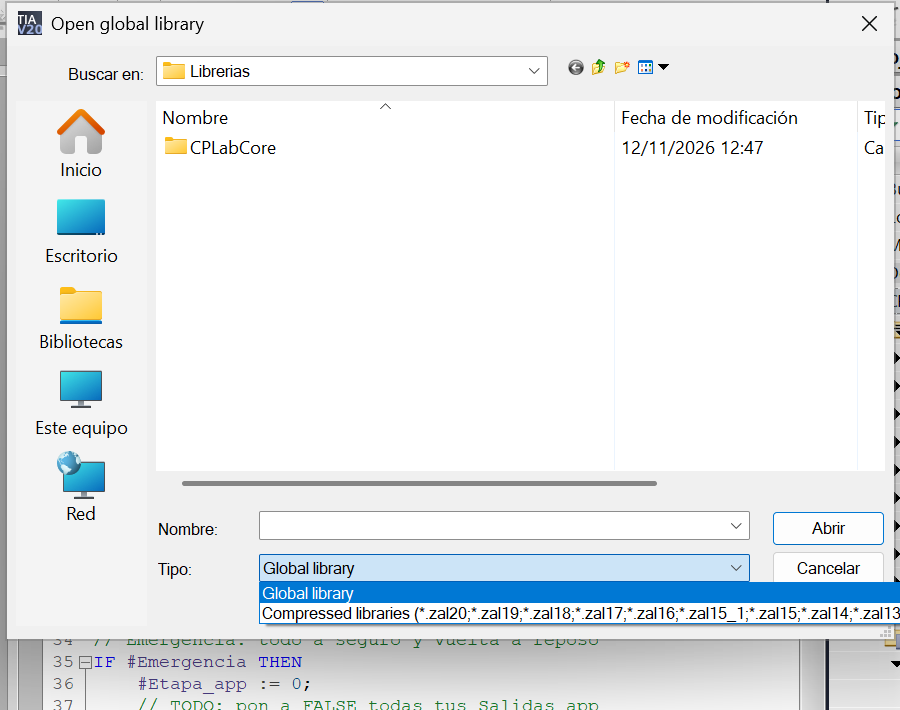
\includegraphics[width=0.78\textwidth]{capturas/abrir_libreria.png}
\caption{El cuadro «Open global library», con la lista de tipos desplegada. El segundo tipo (\textit{Compressed libraries}) es el que hay que elegir para abrir un \texttt{.zal20}.}
\end{figure}

\paso{Elige una carpeta para extraerla}
TIA te pedirá una carpeta donde extraer la librería. Elige una carpeta \textbf{propia y vacía} (por ejemplo, \ruta{C:\textbackslash Librerias\textbackslash CPLabCore}); no la pongas dentro de la carpeta de tu proyecto.

\begin{ojo}
El manual de la CP-Lab explica lo mismo para otra librería con otro nombre de menú: clic derecho en «Librerías globales» y \menu{Desarchivar librería} (en inglés, \textit{Retrieve library}). Según la versión de TIA, el comando está en el botón de abrir o en ese menú contextual. Los dos hacen lo mismo.
\end{ojo}

\comprobar{En la sección \menu{Global libraries} aparece la librería \menu{CPLabCore}. Al desplegarla ves las carpetas \menu{Types} y \menu{Master copies}, como en la figura~\ref{fig:biblioteca}.}

\begin{figure}[ht]
\centering
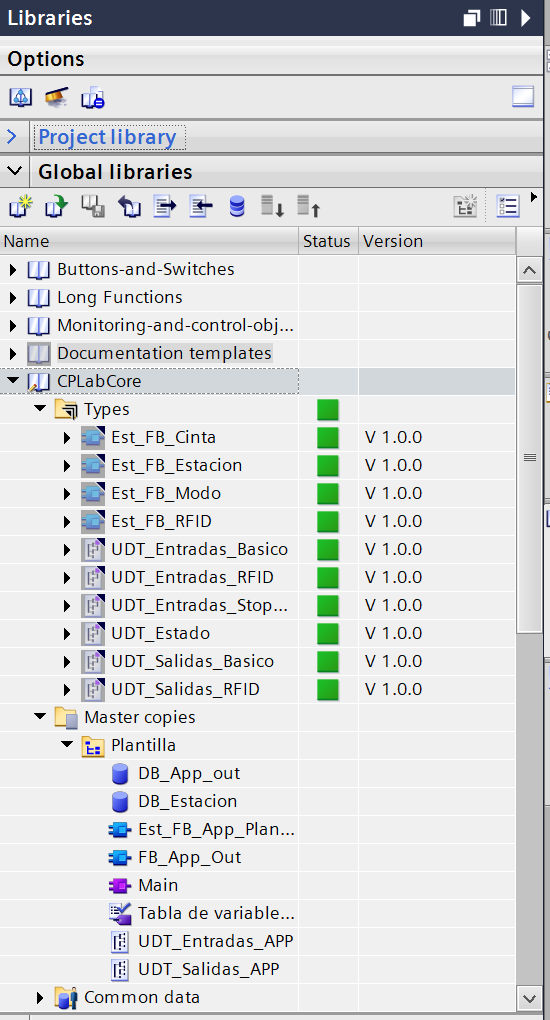
\includegraphics[width=0.62\textwidth]{capturas/biblioteca.png}
\caption{La librería abierta en TIA Portal. En \menu{Types} están los diez tipos, con versión; en \menu{Master copies}, la carpeta \menu{Plantilla}. (Captura de la versión 1.0.0, con el mismo contenido.)}
\label{fig:biblioteca}
\end{figure}

\section{Paso 2: copiar los tipos a tu proyecto}\label{sec:copiar-tipos}
Los tipos se arrastran de la librería al proyecto. Es suficiente arrastrar \textbf{uno}: el bloque \cod{Est\_FB\_Estacion}. TIA añade sola todo lo que necesita.

\paso{Arrastra \cod{Est\_FB\_Estacion}}
En el panel de librerías, abre \menu{CPLabCore $\rightarrow$ Types}. Arrastra \menu{Est\_FB\_Estacion} hasta la carpeta \menu{Program blocks} de tu PLC, en el árbol del proyecto (a la izquierda).

\comprobar{Aparecen en \menu{Program blocks} los cuatro FB (\cod{Est\_FB\_Estacion}, \cod{Est\_FB\_Modo}, \cod{Est\_FB\_Cinta}, \cod{Est\_FB\_RFID}) y en \menu{PLC data types} los seis UDT (\cod{UDT\_Entradas\_Basico}, \cod{UDT\_Entradas\_RFID}, \cod{UDT\_Entradas\_Stopper}, \cod{UDT\_Estado}, \cod{UDT\_Salidas\_Basico} y \cod{UDT\_Salidas\_RFID}).}

\begin{consejo}
Esto se ha comprobado con un proyecto nuevo creado solo para probar la librería: arrastrar \cod{Est\_FB\_Estacion} trajo sus tres FB y sus seis UDT, sin tener que arrastrar ninguno a mano.
\end{consejo}

Los bloques traídos de la librería quedan \textbf{ligados} a ella: en el árbol tienen un icono especial y TIA no deja editarlos desde el proyecto (solo desde la librería). Es lo que se quiere.

\section{Paso 3: copiar la plantilla}\label{sec:copiar-plantilla}
Después se copian de \menu{Master copies $\rightarrow$ Plantilla} las piezas que son tuyas. \textbf{El orden importa} porque unas dependen de otras:

\begin{enumerate}
\item \menu{UDT\_Entradas\_APP} y \menu{UDT\_Salidas\_APP}: los UDT de ejemplo de la aplicación. Solo si los vas a usar como punto de partida; si tu aplicación tiene los suyos, sáltalos.
\item \menu{Tabla de variables estándar}: los siete tags de entradas y salidas (sección~\ref{sec:tags}). Va a \menu{PLC tags}.
\item \menu{DB\_Estacion}: el bloque de datos del contrato.
\item \menu{Est\_FB\_App\_Plantilla}: el esqueleto de aplicación.
\item \menu{Main}: \cod{Main} de ejemplo con las dos llamadas ya cableadas. Si tu proyecto ya tiene un \cod{Main} con tu código, \textbf{no lo sobrescribas todavía}: copia las redes a mano en el capítulo~\ref{cap:migracion}.
\end{enumerate}
Los bloques \menu{FB\_App\_Out} y \menu{DB\_App\_out} son la aplicación completa de la estación Out. Cópialos solo si quieres mirarlos como ejemplo.

\section{Los siete tags de entradas y salidas}\label{sec:tags}
Los tags son lo que enlaza los UDT con los módulos físicos. La copia maestra «Tabla de variables estándar» los trae ya hechos; si prefieres crearlos a mano (por ejemplo, porque tu configuración de hardware es distinta), son estos:

\begin{center}
\small
\begin{tabularx}{\textwidth}{>{\ttfamily}p{3.6cm}>{\ttfamily}p{4.2cm}>{\ttfamily}p{1.9cm}X}
\toprule
\textnormal{\textbf{Nombre}} & \textnormal{\textbf{Tipo de datos}} & \textnormal{\textbf{Dirección}} & \textbf{Módulo} \\
\midrule
Entradas\_APP & UDT\_Entradas\_APP & \%I0.0 & Primer módulo de entradas digitales (tu aplicación). \\
Entradas\_Basico & UDT\_Entradas\_Basico & \%I1.0 & Segundo módulo de entradas (botonera, cinta). \\
Entradas\_Stopper & UDT\_Entradas\_Stopper & \%I42.0 & Dispositivo IO-Link del stopper. \\
Entradas\_RFID & UDT\_Entradas\_RFID & \%I10.0 & Lector RFID por IO-Link. \\
Salidas\_APP & UDT\_Salidas\_APP & \%Q0.0 & Primer módulo de salidas (tu aplicación). \\
Salidas\_Basico & UDT\_Salidas\_Basico & \%Q1.0 & Segundo módulo de salidas (luces, cinta). \\
Salidas\_RFID & UDT\_Salidas\_RFID & \%Q10.0 & Lector RFID por IO-Link. \\
\bottomrule
\end{tabularx}
\end{center}

\begin{ojo}
Son las direcciones de la maqueta real, según el manual de la CP-Lab (apartado 11.2): botonera \cod{\%E1}/\cod{\%A1}, stopper \cod{\%E42}, RFID \cod{\%E10}/\cod{\%A10}, y la aplicación en el primer byte (\cod{\%E0}/\cod{\%A0}). Son \textbf{iguales en todas las estaciones}. Lo único que varía de una estación a otra es el contenido del byte de la aplicación. Si tu proyecto usa otras direcciones (por ejemplo, las del simulador CIROS empiezan en el byte 100), cambia solo la dirección del tag, no el UDT.
\end{ojo}

\section{Paso 4: comprobar que compila}
Compila todo el software del PLC (\menu{Compile $\rightarrow$ Software (rebuild all blocks)}). Qué esperar:

\begin{itemize}
\item \textbf{0 errores} si has copiado la tabla de variables. Es normal un aviso general del estilo «Inputs or outputs are used that do not exist in the configured hardware»: significa que algún tag apunta a una dirección que tu configuración de hardware no tiene todavía. Se resuelve en el capítulo~\ref{cap:migracion}.
\item Si no has copiado los tags, el error es \cod{Tag "Entradas\_Basico" not defined} (y los otros seis). Es exactamente lo que se ve al instalar en un proyecto vacío sin la tabla de variables; no indica ningún problema en la librería.
\end{itemize}

\section{Qué se ha comprobado en la instalación}
Con el archivo de la librería, y desde una instalación aparte (como la haría uno de nosotros), se ha comprobado:
\begin{enumerate}
\item La librería se desarchiva y se abre sin errores.
\item Al arrastrar \cod{Est\_FB\_Estacion} a un proyecto nuevo con una CPU \texttt{1512SP F-1 PN}, aparecen sus tres FB y sus seis UDT.
\item Las copias maestras (los dos UDT de aplicación, \cod{FB\_App\_Out}, \cod{Est\_FB\_App\_Plantilla}, \cod{DB\_App\_out}, \cod{DB\_Estacion} y \cod{Main}) se copian al proyecto.
\item Los tres ejemplos de aplicación (Press, BackCover y Cámara) compilan sin errores en TIA.
\end{enumerate}
La copia de la \emph{tabla de variables} se hace en la interfaz de TIA, arrastrándola. Es la única copia maestra que no se pudo comprobar de forma automática; si no se copiara, la tabla de la sección anterior tiene los siete tags para crearlos a mano.

\section{Actualizar a una versión nueva}
Cuando salga una versión nueva de la librería (capítulo~\ref{cap:mantenimiento}):
\begin{enumerate}
\item Desarchiva el nuevo \texttt{.zal20} como en el paso 1, en una carpeta nueva.
\item En el panel de librerías, haz clic derecho sobre la librería y usa \menu{Update types} (Actualizar tipos): TIA muestra qué tipos de tu proyecto tienen una versión nueva y los actualiza.
\item Vuelve a compilar y repite las pruebas de aceptación (capítulo~\ref{cap:pruebas}).
\end{enumerate}
Como los tipos están ligados a la librería, no pierdes nada tuyo: tus aplicaciones, tu \cod{Main} y tus tags no se tocan.

\chapter{Migrar tu estación a la librería}\label{cap:migracion}

Este es el capítulo para el que se ha hecho todo lo demás. Cuenta, paso a paso, cómo llevar tu estación a \lib\ \textbf{sea cual sea el punto en el que estés}: si no has empezado, si lo tienes todo mezclado en un bloque enorme, o si ya tienes una estructura parecida a la de la práctica.

\begin{idea}
La migración no consiste en \emph{reescribir} tu estación, sino en \textbf{separarla en dos}: lo común (que ahora lo hace la librería, y que tú borras) y lo propio (tu aplicación, que conservas y adaptas). Casi todo el trabajo es decidir qué parte de tu código es cuál.
\end{idea}

\section{Antes de empezar}

\subsection{Las cinco fases}
\begin{figure}[ht]
\centering
\begin{tikzpicture}[x=1cm,y=1cm]
\newcommand{\fase}[5]{\node[#2,minimum width=2.45cm,minimum height=1.9cm,font=\sffamily\footnotesize,text width=2.2cm,align=center] (f#1) at (#1*2.9-5.8,0) {\textbf{#1}\\[-1pt]\textbf{#3}\\[1pt]{\scriptsize #4}};}
\fase{1}{caja}{Preparar}{copia de seguridad, inventario, hardware}{}
\fase{2}{libcaja}{Instalar}{la librería y los tags (cap.\ \ref{cap:instalacion})}{}
\fase{3}{caja}{Separar}{qué se va y qué se queda de tu código}{}
\fase{4}{appcaja}{Reconstruir}{tu aplicación con el contrato}{}
\fase{5}{caja}{Conectar y probar}{\cod{Main} y pruebas}{}
\foreach \i/\j in {1/2,2/3,3/4,4/5} \draw[flecha] (f\i.east) -- (f\j.west);
\end{tikzpicture}
\caption{Las cinco fases de la migración. Entre una y otra se compila: no sigas si hay errores.}
\end{figure}

\subsection{Cuánto tiempo lleva}
Con el código que ya tienes, calcula entre dos y cuatro horas la primera vez: una para preparar e instalar, una a dos para separar y reconstruir, y una para probar. La primera estación de cada uno es la lenta; el resto de la gente va más deprisa porque ya ha visto el patrón.

\subsection{Cuatro normas}
\begin{enumerate}[leftmargin=1.2cm,label=\textbf{N\arabic*.}]
\item \textbf{Copia de seguridad antes de tocar nada.} Archiva tu proyecto (\menu{Project $\rightarrow$ Archive}) con la fecha en el nombre.
\item \textbf{No borres tu código antiguo: apártalo.} Crea una carpeta \menu{Antiguo} dentro de \menu{Program blocks} y mueve ahí lo que sustituyas. Hasta que todo funcione, es tu red de seguridad.
\item \textbf{Un paso cada vez y compilando.} Así sabes siempre qué cambio ha roto algo.
\item \textbf{No edites los bloques de la librería.} Si algo no te encaja, mira el capítulo~\ref{cap:problemas} o pide un cambio (capítulo~\ref{cap:mantenimiento}).
\end{enumerate}

\section{¿En qué punto estás?}\label{sec:punto}
Elige la fila que más se parezca a tu situación. Cada una te manda al camino que debes seguir.

\begin{center}
\small
\begin{tabularx}{\textwidth}{>{\bfseries}p{4.1cm}Xp{2.0cm}}
\toprule
Tu situación & Qué hacer & Camino \\
\midrule
Solo tienes el hardware configurado, o muy poco programado & Empieza con la plantilla. Es lo más fácil. & A (sección~\ref{sec:camino-a}) \\
Tienes la estructura de la práctica: bloques separados de modos, cinta, RFID y aplicación & Sustituye los tres primeros por la librería; conserva y adapta tu aplicación. & B (sección~\ref{sec:camino-b}) \\
Tienes todo en uno o dos bloques, mezclado & Primero hay que separar (sección~\ref{sec:separar}), y luego sigues el camino B. & B, con separación \\
Tu código ya lee o escribe el tag RFID a su manera (una palabra, otra dirección, otro formato) & Sigue el camino que te toque y haz además la sección~\ref{sec:rfid-propio}. & A o B, más \S\,\ref{sec:rfid-propio} \\
Tu estación tiene hardware especial (cámara PROFINET, PLC Festo…) & Sigue igual: ese hardware es parte de tu aplicación, la librería no lo toca. & A o B \\
\bottomrule
\end{tabularx}
\end{center}

\begin{figure}[ht]
\centering
\begin{tikzpicture}[x=1cm,y=1cm]
\node[caja,fill=white] (q1) at (0,0) {¿Tu proyecto ya tiene programados\\los botones, la cinta y el RFID?};
\node[libcaja] (A) at (-6.0,0) {\textbf{Camino A}\\proyecto nuevo\\con la plantilla};
\node[caja,fill=white] (q2) at (0,-2.4) {¿Tu aplicación está en un bloque\\propio, separada de lo anterior?};
\node[libcaja] (B) at (6.0,-2.4) {\textbf{Camino B}\\sustituir lo común,\\adaptar tu aplicación};
\node[appcaja] (S) at (0,-4.9) {\textbf{Camino B con separación}\\(antes, separar tu código en\\«lo común» y «lo propio»)};
\draw[flecha] (q1.west) -- node[etiqueta,above] {no} (A.east);
\draw[flecha] (q1.south) -- node[etiqueta,right] {sí} (q2.north);
\draw[flecha] (q2.east) -- node[etiqueta,above] {sí} (B.west);
\draw[flecha] (q2.south) -- node[etiqueta,right] {no, está todo mezclado} (S.north);
\draw[flecha] (S.east) -| (B.south);
\end{tikzpicture}
\caption{Cómo elegir el camino.}
\end{figure}

\section{Camino A: empezar con la plantilla}\label{sec:camino-a}
Es el camino corto: tu proyecto casi no tiene lógica, así que se construye todo sobre la librería desde el principio. Calcula una hora u hora y media.

\reiniciapaso
\paso{Prepara el proyecto}
Crea un proyecto con tu CPU y configura el hardware de la estación: las dos tarjetas de entradas, las dos de salidas y el maestro IO-Link con el lector y el stopper. Las direcciones tienen que ser las de la tabla de la sección~\ref{sec:tags}. Si ya tienes un proyecto con el hardware hecho (por ejemplo, el de la práctica), úsalo y borra lo demás.

\paso{Instala la librería}
Capítulo~\ref{cap:instalacion}: desarchivar, arrastrar \cod{Est\_FB\_Estacion} y copiar de la plantilla los tags, \cod{DB\_Estacion}, \cod{Est\_FB\_App\_Plantilla} y \cod{Main}.

\paso{Crea tus señales físicas}
Haz el inventario (lista~1 de la sección~\ref{sec:fase1}) y crea los tags de tus sensores y actuadores, con un UDT propio o sueltos.

\paso{Convierte la plantilla en tu aplicación}
Copia \cod{Est\_FB\_App\_Plantilla}, renómbrala \cod{FB\_App\_}\emph{tu estación} y sigue los seis pasos de la fase~4 (sección~\ref{sec:fase4}): tus señales, tus bytes del tag, tu condición de reposo y tu secuencia.

\paso{Conecta y calcula tus máscaras}
En \cod{Main}, cambia la llamada de la plantilla por tu aplicación y pon tus máscaras (capítulo~\ref{cap:mapa}). Si tu aplicación tiene señales físicas, cablea esos pines a tus tags (sección~\ref{sec:fase5}).

\paso{Compila y prueba}
Compila y haz las pruebas del capítulo~\ref{cap:pruebas}, empezando por la escritura desactivada.

\comprobar{Compila con 0 errores y las 12 pruebas de aceptación pasan.}

\section{Camino B: migrar un proyecto existente}\label{sec:camino-b}
Es el camino largo, pero se hace en cinco fases que conviene hacer \textbf{en este orden}. Cada fase termina con una comprobación: si no la cumples, no sigas.

\section{Fase 1: preparar}\label{sec:fase1}
\reiniciapaso
\paso{Haz la copia de seguridad}
\menu{Project $\rightarrow$ Archive}, tipo \menu{Compressed TIA Portal project archive}, con un nombre como \texttt{MiEstacion\_antes\_de\_CPLabCore.zap20}.

\paso{Rellena el inventario de tu estación}
Es una hoja con cuatro listas (la versión imprimible está en el apéndice~\ref{ap:checklists}). Es lo más útil de toda la migración, porque te obliga a decidir qué es tuyo y qué es común:

\begin{center}
\small
\begin{tabularx}{\textwidth}{>{\bfseries}p{4.2cm}X}
\toprule
Lista & Qué apuntar \\
\midrule
1. Mis señales físicas & Todos los sensores y actuadores que \textbf{no} son botonera, cinta, stopper ni RFID. Con su dirección actual. (Esas son tu aplicación.) \\
2. Mis datos del palet & Qué información lees del tag y cuál escribes. Con su byte según el Excel del grupo (capítulo~\ref{cap:mapa}). \\
3. Cuándo puedo empezar & La condición que tiene que cumplir tu mecanismo para estar en reposo y recibir un palet. \\
4. Cuándo he terminado & La condición con la que sabes que has acabado con el palet. \\
\bottomrule
\end{tabularx}
\end{center}

\paso{Comprueba tu hardware}
Abre \menu{Device configuration} y comprueba que tus módulos tienen las direcciones de la tabla de la sección~\ref{sec:tags}: entradas digitales en 0 y 1, salidas digitales en 0 y 1, y el maestro IO-Link con el lector en 10 y el stopper en 42. Son las mismas en todas las estaciones de la CP-Lab. Si alguna es distinta, apúntala: en la fase 2 la corregirás en el tag, no en la librería.

\comprobar{Tienes la copia, el inventario relleno y la lista de direcciones que no coinciden (si hay alguna).}

\section{Fase 2: instalar}
Sigue el capítulo~\ref{cap:instalacion}: desarchivar la librería, arrastrar \cod{Est\_FB\_Estacion} (con sus dependencias) y copiar los tags y los bloques de la plantilla. Algunas notas especiales para un proyecto que ya tiene cosas:

\begin{itemize}
\item \textbf{Tags que ya tengas con las mismas direcciones.} Si en tu tabla de variables hay tags sueltos para los botones, la cinta o el RFID (por ejemplo, \cod{Boton\_marcha} en \cod{\%I1.0}), son los que sustituyen los siete tags de la librería. Muévelos a otra tabla (\menu{Antiguo}) o desactívalos; no los borres de momento, porque tu código antiguo los usa. La librería usa tags \emph{con estructura} en esas direcciones.
\item \textbf{Tu aplicación sigue con sus propios tags} y UDT: no les afecta nada de esto.
\item \textbf{Bloques con los mismos nombres.} Si ya tienes un \cod{Main} o un \cod{FB1}, TIA te preguntará qué hacer al copiar. En el \cod{Main}, no sobrescribas todavía.
\end{itemize}

\comprobar{El software compila y no hay errores en los bloques de la librería. Los errores que queden son de tu código antiguo (que usa nombres que ya no existen) y se resuelven en la fase 3.}

\section{Fase 3: separar tu código}\label{sec:separar}
Es el momento de decidir, línea a línea, qué se queda y qué se va. La regla es sencilla:

\begin{idea}
\textbf{Si el código tiene que ver con los botones, la cinta, el stopper, el lector RFID o la secuencia «leer, trabajar, escribir», ya lo hace la librería: sobra. Si mueve tu mecanismo o inspecciona, pone o procesa una pieza, es tu aplicación: se queda.}
\end{idea}

La tabla de la página siguiente traduce las cosas más habituales. Mira cada parte de tu código y búscala en la columna izquierda.

\begin{center}
\small
\begin{longtable}{>{\raggedright\arraybackslash}p{5.6cm}>{\raggedright\arraybackslash}p{2.0cm}>{\raggedright\arraybackslash}p{6.2cm}}
\toprule
\textbf{Si tu código hace\dots} & \textbf{Qué hacer} & \textbf{Ahora lo hace\dots} \\
\midrule\endhead
Leer el botón de marcha, paro o rearme, el selector manual/auto o la seta & \textcolor{rojo}{Borrar} & \cod{Est\_FB\_Modo}. Entradas en \cod{Entradas\_Basico}. \\
Decidir si hay emergencia y cómo se sale de ella & \textcolor{rojo}{Borrar} & \cod{Est\_FB\_Modo}. Tu aplicación recibe \cod{Emergencia}. \\
Encender las luces de marcha, rearme, ciclo y emergencia & \textcolor{rojo}{Borrar} & \cod{Est\_FB\_Estacion}. Tú puedes pedir rearme con \cod{App\_rearme\_requerido} y alarma con \cod{App\_alarma}. \\
Mover la cinta, bajar o subir el stopper, contar palets & \textcolor{rojo}{Borrar} & \cod{Est\_FB\_Cinta}. Si tu mecanismo estorba, \cod{Inhibir\_cinta}. \\
Detectar que el palet ha llegado al tope & \textcolor{rojo}{Borrar} & \cod{Est\_FB\_Cinta}: \cod{Palet\_en\_posicion}. La aplicación empieza con \cod{App\_inicio}. \\
Dar la orden de leer el RFID, esperar el resultado, gestionar errores y tiempos & \textcolor{rojo}{Borrar} & \cod{Est\_FB\_RFID}. \\
Dar la orden de escribir el RFID y esperar el resultado & \textcolor{rojo}{Borrar} & \cod{Est\_FB\_RFID}. \\
La secuencia «llega palet, leer, trabajar, escribir, soltar» & \textcolor{rojo}{Borrar} & \cod{Est\_FB\_Estacion} (la secuencia del palet). \\
Una condición como «puedo arrancar» & \textcolor{azul}{Convertir} & \cod{App\_en\_reposo}. \\
Una señal como «he terminado» & \textcolor{azul}{Convertir} & \cod{App\_terminada} (y mantenerla hasta que \cod{App\_inicio} baje). \\
Usar datos que leíste del tag (por ejemplo, la calidad) & \textcolor{azul}{Convertir} & Leer \cod{Imagen\_palet[n]}. El byte tiene que estar en \cod{Mascara\_lectura}. \\
Guardar resultados en el tag & \textcolor{azul}{Convertir} & Escribir \cod{Imagen\_palet[n]}. El byte tiene que estar en \cod{Mascara\_escritura}. \\
Parar tus actuadores en emergencia & \textcolor{verde!60!black}{Conservar} & Dentro de tu aplicación, con la señal \cod{Emergencia}. \\
Mover tu mecanismo, activar tus sensores y actuadores, temporizar tus pasos & \textcolor{verde!60!black}{Conservar} & Dentro de tu aplicación, en el estado de «trabajo». \\
Mostrar cosas en la HMI & \textcolor{verde!60!black}{Conservar} & Tu HMI lee las variables de tu aplicación, o \cod{DB\_Estacion}. La librería no toca la HMI. \\
Contadores de piezas, estadísticas, registros & \textcolor{verde!60!black}{Conservar} & En tu aplicación o en tu propio bloque. \\
\bottomrule
\end{longtable}
\end{center}

\begin{ojo}
\textcolor{rojo}{\textbf{Borrar}} no significa eliminarlo ya: significa que \emph{sobra}. Muévelo a la carpeta \menu{Antiguo}. \textcolor{azul}{\textbf{Convertir}} significa que la idea se queda, pero ahora se expresa con una señal del contrato. \textcolor{verde!60!black}{\textbf{Conservar}} es tu aplicación.
\end{ojo}

\subsection{Si tienes todo mezclado en un solo bloque}
Es el caso más frecuente en los primeros intentos y no es un problema, solo requiere un paso más. Recomendación:

\paso{Duplica el bloque grande}
Haz una copia con otro nombre (por ejemplo, \cod{FB\_Antiguo}). Trabaja sobre la copia para tener siempre el original.

\paso{Marca con comentarios}
Recorre el código y pon al margen una etiqueta en cada tramo: \texttt{//[BORRAR]}, \texttt{//[CONVERTIR]} o \texttt{//[APP]}, según la tabla anterior.

\paso{Pasa a un bloque nuevo solo lo que sea \texttt{[APP]} o \texttt{[CONVERTIR]}}
Crea la aplicación nueva con la plantilla (fase 4) y copia ahí únicamente esos tramos. El resto no se copia.

\comprobar{Tienes dos cosas: un bloque antiguo apartado, intacto, y una lista clara (los comentarios) de qué parte pasa a la aplicación.}

\section{Fase 4: reconstruir tu aplicación}\label{sec:fase4}
Aquí se construye tu aplicación sobre la plantilla. Se hace en seis pasos.

\reiniciapaso
\paso{Copia la plantilla con tu nombre}
Copia \cod{Est\_FB\_App\_Plantilla} y renómbrala \cod{FB\_App\_}\emph{tu estación} (por ejemplo, \cod{FB\_App\_Press}). Se queda como bloque tuyo, sin vínculo con la librería.

\paso{Añade tus señales físicas a la interfaz}
En el apartado \texttt{VAR\_INPUT} añade tus sensores, y en \texttt{VAR\_OUTPUT} tus actuadores (con un tipo \texttt{Bool}, o el que necesites). Sácalos de tu inventario, lista~1. Los ejemplos del apéndice~\ref{ap:listados} lo hacen así y es la forma más sencilla: la aplicación no depende de ningún UDT y el cableado se hace en \cod{Main}.

\begin{consejo}
Si ya tienes un UDT con tus entradas y salidas (como \cod{UDT\_Entradas\_APP}), puedes dejarlo: usa \cod{Entradas\_app} y \cod{Salidas\_app} con ese tipo, y cablea los tags en \cod{Main}. Es lo que hace \cod{FB\_App\_Out}.
\end{consejo}

\paso{Declara tus bytes del tag}
En \texttt{VAR CONSTANT} escribe un \cod{IDX\_...} por cada byte que lees o escribes (inventario, lista~2), con el número de byte del Excel. Y apunta también los bits que uses, como \cod{BIT\_PRESS}. Cada byte que escribas tiene que estar en tu \cod{Mascara\_escritura}; cada byte que leas o escribas, en tu \cod{Mascara\_lectura}. Calcula las máscaras con el método de la sección~\ref{sec:calculo-mascara}.

\paso{Traslada tu condición de reposo}
En el estado 0 de la plantilla, sustituye \cod{App\_en\_reposo := TRUE} por tu condición (inventario, lista~3): por ejemplo, «prensa arriba» o «garra abierta y eje referenciado».

\paso{Traslada tu secuencia al estado de trabajo}
Pega la secuencia de tu mecanismo (lo marcado \texttt{[APP]}) dentro del estado 10 de la plantilla. Si tiene varias etapas, convierte el estado 10 en varios (10, 20, 30\dots), y cuando acabe la última, salta al estado de fin. En cada etapa donde antes leías el tag, usa \cod{Imagen\_palet[IDX\_...]}; donde lo escribías, asigna a la imagen.

\paso{Termina bien: resultado y mantén}
Antes del estado de fin, deja escritos en la imagen todos tus resultados. En el estado de fin, la plantilla ya hace lo correcto: \cod{App\_terminada} verdadera hasta que \cod{App\_inicio} baje, y vuelta a reposo. No lo cambies.

\comprobar{Tu aplicación compila sola. Ya cumple el contrato (revisa las cinco comprobaciones al final del capítulo~\ref{cap:contrato}).}

\subsection{Un ejemplo de antes y después}
Para ver el patrón, aquí va un caso inventado y simplificado de una estación de prensa programada «a la antigua», con todo mezclado, y cómo queda con la librería. No es ningún proyecto real: sirve para ver qué se va y qué se queda.

\begin{lstlisting}[caption={Antes: todo mezclado (ejemplo ilustrativo).}]
CASE #etapa OF
  0: // esperar
     IF #Boton_marcha AND NOT #Emergencia THEN #etapa := 1; END_IF;       // [BORRAR] botonera
  1: // llega palet
     #Cinta := TRUE;                                                       // [BORRAR] cinta
     IF #Sensor_tope THEN #Cinta := FALSE; #etapa := 2; END_IF;            // [BORRAR]
  2: // leer RFID
     #Tag_leer := TRUE; #Tag_direccion := 0;                               // [BORRAR] RFID
     IF #Tag_leido AND #Tag_listo THEN                                     // [BORRAR]
        #Golpes := #Tag_datos[13];                                         // [CONVERTIR] leer byte 13
        #etapa := 3;
     END_IF;
  3: // prensar
     #Prensa_bajar := TRUE;                                                // [APP]
     IF #Prensa_abajo THEN #Prensa_bajar := FALSE; #etapa := 4; END_IF;    // [APP]
  4: // escribir RFID
     #Tag_datos_a_escribir[16] := #Golpes;                                 // [CONVERTIR] escribir byte 16
     #Tag_escribir := TRUE;                                                // [BORRAR]
     IF #Tag_escrito THEN #etapa := 5; END_IF;                             // [BORRAR]
  5: // soltar palet
     #Stopper_bajar := TRUE; #Cinta := TRUE;                               // [BORRAR]
END_CASE;
\end{lstlisting}

\begin{lstlisting}[caption={Después: solo la aplicación (el patrón; el ejemplo completo está en el apéndice).}]
CASE #Etapa_app OF
  0: #App_en_reposo := #Prensa_arriba;                                    // tu condicion de reposo
     IF #App_inicio AND #App_en_reposo THEN
        #Golpes_pedidos := BYTE_TO_INT(#Imagen_palet[#IDX_NUM_GOLPES]);    // leer del tag = leer la imagen
        #Etapa_app := 10;
     END_IF;
  10: #Prensa_bajar := TRUE;                                              // tu mecanismo, igual que antes
      IF #Prensa_presion_inferior THEN #Etapa_app := 40; END_IF;
  40: #Imagen_palet[#IDX_GOLPES_HECHOS] := INT_TO_BYTE(#Golpes_hechos);    // escribir en el tag = escribir la imagen
      #Etapa_app := 50;
  50: #App_terminada := TRUE;                                              // fin: se mantiene hasta que App_inicio baje
      IF NOT #App_inicio THEN #Etapa_app := 0; END_IF;
END_CASE;
\end{lstlisting}

Casi todo lo que hacía el bloque antiguo (botón de marcha, cinta, tope, lectura y escritura del RFID, soltar el palet) ya no está: lo hace la librería. Lo único que queda es lo que sabe hacer la prensa.

\section{Fase 5: conectar en \texttt{Main}}\label{sec:fase5}
\cod{Main} tiene dos llamadas, siempre en este orden: primero la librería y luego tu aplicación. Si copiaste el \cod{Main} de la plantilla, ya las tienes; solo te quedan tus señales físicas.

\begin{figure}[ht]
\centering
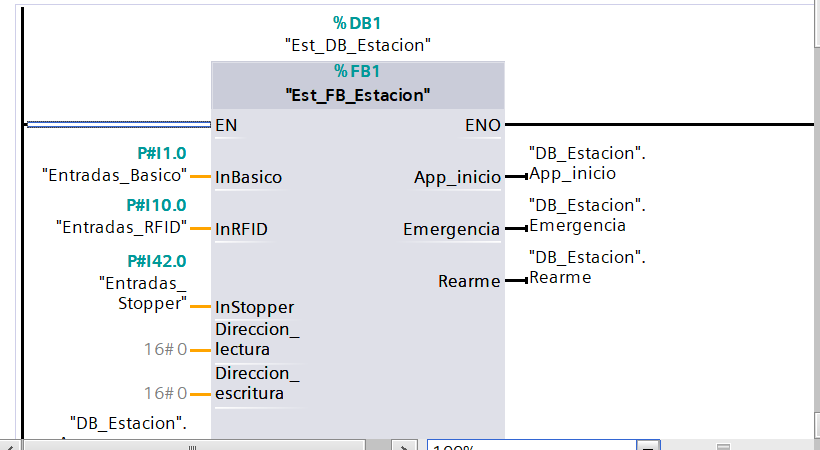
\includegraphics[width=0.92\textwidth]{capturas/main_red1.png}
\caption{La llamada a \cod{Est\_FB\_Estacion} en \cod{Main} (captura de TIA Portal). A la izquierda, las entradas; a la derecha, las salidas. Los valores \texttt{16\#0000}, \texttt{16\#00620220} y \texttt{16\#0FFFFFFF} son los de la estación Out.}
\end{figure}

\subsection{Red 1: la librería}
Llama a \cod{Est\_FB\_Estacion} con su bloque de datos de instancia (TIA lo crea) y cablea cada pin así:

\begin{center}
\footnotesize
\begin{tabularx}{\textwidth}{>{\ttfamily}p{3.5cm}>{\ttfamily}p{5.3cm}X}
\toprule
\textnormal{\textbf{Pin}} & \textnormal{\textbf{Conéctalo a}} & \textbf{Notas} \\
\midrule
InBasico & "Entradas\_Basico" & Igual en todas las estaciones. \\
InRFID & "Entradas\_RFID" & Igual en todas. \\
InStopper & "Entradas\_Stopper" & Igual en todas. \\
Direccion\_lectura & 16\#0000 & Dirección de inicio del bloque (sección~\ref{sec:calculo-mascara}). \\
Direccion\_escritura & 16\#0000 & Igual que la anterior. \\
Mascara\_lectura & \textbf{la tuya} & Capítulo~\ref{cap:mapa}. \\
Mascara\_escritura & \textbf{la tuya} & Capítulo~\ref{cap:mapa}. \\
App\_en\_reposo & "DB\_Estacion".App\_en\_reposo & Contrato. \\
App\_terminada & "DB\_Estacion".App\_terminada & Contrato. \\
App\_alarma & "DB\_Estacion".App\_alarma & Contrato. \\
App\_rearme\_requerido & "DB\_Estacion".App\_rearme\_requerido & Contrato. \\
Inhibir\_cinta & "DB\_Estacion".Inhibir\_cinta & Contrato. \\
App\_inicio (salida) & "DB\_Estacion".App\_inicio & Contrato. \\
Emergencia (salida) & "DB\_Estacion".Emergencia & Contrato. \\
Rearme (salida) & "DB\_Estacion".Rearme & Contrato. \\
OutBasico & "Salidas\_Basico" & Igual en todas. \\
OutRFID & "Salidas\_RFID" & Igual en todas. \\
Imagen\_palet & "DB\_Estacion".Imagen\_palet & La imagen del palet. \\
\bottomrule
\end{tabularx}
\end{center}

\subsection{Red 2: tu aplicación}
Llama a tu bloque \cod{FB\_App\_}\emph{tu estación} y cablea las señales del contrato a las mismas variables de \cod{DB\_Estacion}:

\begin{center}
\footnotesize
\begin{tabularx}{\textwidth}{>{\ttfamily}p{3.5cm}>{\ttfamily}p{5.3cm}X}
\toprule
\textnormal{\textbf{Pin de tu aplicación}} & \textnormal{\textbf{Conéctalo a}} & \textbf{Dirección} \\
\midrule
App\_inicio & "DB\_Estacion".App\_inicio & entrada \\
Emergencia & "DB\_Estacion".Emergencia & entrada \\
Rearme & "DB\_Estacion".Rearme & entrada \\
App\_en\_reposo & "DB\_Estacion".App\_en\_reposo & salida \\
App\_terminada & "DB\_Estacion".App\_terminada & salida \\
App\_alarma & "DB\_Estacion".App\_alarma & salida \\
App\_rearme\_requerido & "DB\_Estacion".App\_rearme\_requerido & salida \\
Inhibir\_cinta & "DB\_Estacion".Inhibir\_cinta & salida \\
Imagen\_palet & "DB\_Estacion".Imagen\_palet & entrada/salida \\
\textit{(tus señales físicas)} & \textit{tus tags} & según tu estación \\
\bottomrule
\end{tabularx}
\end{center}

\begin{consejo}
Cablea los pines de tus señales físicas \textbf{directamente a los tags de tu módulo}, por ejemplo \cod{"Entradas\_APP".Eje\_z\_arriba}. Es la manera más clara: ves de un vistazo qué sensor entra en qué pin.
\end{consejo}

\paso{Compila}
Compila todo el software. Los errores típicos de esta fase y su solución están en el capítulo~\ref{cap:problemas}.

\comprobar{0 errores. Un aviso sobre direcciones de hardware que no existen es normal si aún no has ajustado tu configuración.}

\section{Datos del RFID con un formato propio}\label{sec:rfid-propio}
Si tu código antiguo ya trabajaba con el tag a su manera, esto es lo que hay que cambiar según el caso.

\begin{description}[style=nextline,leftmargin=1.2cm]
\item[Leías el array de 28 bytes directamente (\cod{Entradas\_RFID.Tag\_datos\_leidos\_escritos[n]}).] Sustitúyelo por \cod{Imagen\_palet[n]}. El índice $n$ es el mismo (es el offset dentro del bloque). Añade el byte $n$ a \cod{Mascara\_lectura}.
\item[Usabas una palabra (un \texttt{Word} o un \texttt{Int}) en una dirección.] Es lo que hacía la práctica con CIROS. Ahora hay que partirla en dos bytes. Con el formato del grupo (big-endian), la palabra de los bytes $n$ y $n+1$ es:
\begin{lstlisting}
#valor := WORD_TO_INT(SHL(IN := BYTE_TO_WORD(#Imagen_palet[#IDX_ALTO]), N := 8)
                      OR BYTE_TO_WORD(#Imagen_palet[#IDX_BAJO]));
\end{lstlisting}
y al revés, para escribirla, con \cod{\#Imagen\_palet[\#IDX\_ALTO]} y \cod{[\#IDX\_BAJO]} cogiendo el byte alto y el bajo del valor. Los dos bytes tienen que estar en tus máscaras.
\item[Leías en otra dirección distinta de 0.] Pon esa dirección en \cod{Direccion\_lectura} y \cod{Direccion\_escritura} (las dos iguales). Los índices de la imagen son \emph{relativos al comienzo del bloque}: el byte 0 de la imagen es el primero del bloque, estés donde estés en el tag.
\item[Tu estación guardaba cosas en bytes que el mapa no contempla.] No lo hagas sin acordarlo: habla con el grupo, añade el campo al Excel (capítulo~\ref{cap:mapa}) y entonces úsalo.
\item[Necesitas más de 28 bytes.] No es posible con esta versión: el bloque es de 28 bytes. Habría que plantear una versión nueva de la librería (capítulo~\ref{cap:mantenimiento}).
\end{description}

\section{Tres ejemplos resueltos}
El apéndice~\ref{ap:listados} trae tres aplicaciones de ejemplo completas, con la parte del tag ya hecha según el Excel. Son \textbf{puntos de partida}: la parte física (nombres de sensores y actuadores) es de ejemplo y cada grupo la sustituye por la suya. Los tres compilan en TIA y se han probado en el simulador de la librería.

\begin{center}
\small
\begin{tabularx}{\textwidth}{>{\bfseries}p{2.4cm}p{3.7cm}X}
\toprule
Estación & Qué hace con el tag & Estados de la aplicación \\
\midrule
Press (\cod{FB\_App\_Press\_Ejemplo}) & Lee golpes y tiempo; escribe golpes realizados y su bit de «completada». & Reposo $\rightarrow$ bajar $\rightarrow$ mantener $\rightarrow$ subir (se repite $n$ veces) $\rightarrow$ escribir $\rightarrow$ fin. \\
BackCover (\cod{FB\_App\_BackCover\_Ejemplo}) & Marca estado de la tapa trasera (requerida, colocada, falta stock) y su bit. & Reposo $\rightarrow$ colocar (o falta stock) $\rightarrow$ fin. \\
Cámara (\cod{FB\_App\_Camara\_Ejemplo}) & Inicializa el bloque si está vacío; elige el job; escribe resultado, calidad, ImageID e intentos. & Reposo $\rightarrow$ inspeccionar $\rightarrow$ resultado $\rightarrow$ fin (con fallo posible). \\
\bottomrule
\end{tabularx}
\end{center}

\subsection{Qué comparten los tres}
Los tres siguen la misma estructura, que es la que te recomiendo para tu propia aplicación:
\begin{enumerate}
\item Las salidas se ponen a su valor seguro al principio de cada ciclo; cada estado activa las que necesite.
\item En el reposo, antes de empezar, se comprueba si la estación se pide (\emph{«estaciones a realizar»}, byte 3). Si no se pide, el palet pasa sin tocar nada. Esto lo exige el mapa del grupo: un byte 3 a 0 significa que actúan todas.
\item Solo se marca el bit de «completada» (byte 4) si de verdad se ha hecho el trabajo.
\item El estado de fin mantiene \cod{App\_terminada} hasta que \cod{App\_inicio} baja.
\item Emergencia: vuelta a reposo y actuadores apagados.
\end{enumerate}

\subsection{Cómo cablear sus señales físicas en \texttt{Main}}
Por ejemplo, la llamada de Press añade, a los nueve pines del contrato, estas señales propias:
\begin{center}
\small
\begin{tabularx}{\textwidth}{>{\ttfamily}p{4.4cm}>{\ttfamily}p{4.4cm}X}
\toprule
\textnormal{\textbf{Pin (de ejemplo)}} & \textnormal{\textbf{Tu tag}} & \textbf{Qué es} \\
\midrule
Prensa\_arriba & "Entradas\_APP".\textit{tu sensor} & Final de carrera superior. \\
Prensa\_presion\_inferior & "Entradas\_APP".\textit{tu sensor} & Presión inferior alcanzada. \\
Hay\_tapa\_trasera & "Entradas\_APP".\textit{tu sensor} & Hay tapa trasera en el palet. \\
Prensa\_bajar (salida) & "Salidas\_APP".\textit{tu actuador} & Bajar la prensa. \\
Prensa\_subir (salida) & "Salidas\_APP".\textit{tu actuador} & Subir la prensa. \\
\bottomrule
\end{tabularx}
\end{center}

\section{Casos especiales}
\begin{description}[style=nextline,leftmargin=1.2cm]
\item[Tu mecanismo estorba a la cinta.] Activa \cod{Inhibir\_cinta} mientras estorbe. Out lo hace con el eje Z: la cinta solo se mueve con Z arriba.
\item[Tu estación necesita rearmarse tras una emergencia que la deja a medias.] Activa \cod{App\_rearme\_requerido} hasta que te hayas recolocado, y mantén \cod{App\_en\_reposo} a falso. Mira cómo lo hace \cod{FB\_App\_Out} (estado 30).
\item[Quieres avisar de un problema sin parar la estación.] \cod{App\_alarma}. Si la haces parpadear en tu aplicación, la luz Q2 parpadea.
\item[Tu estación no usa cinta (por ejemplo, un puesto manual).] La librería no está pensada para eso; habla con el grupo antes de adaptarla.
\item[Quieres leer o escribir el tag más de una vez por palet.] La secuencia de la librería lee una vez y escribe una vez. Si necesitas algo distinto, es un cambio de la librería (capítulo~\ref{cap:mantenimiento}).
\item[Tu estación tiene una HMI propia.] La HMI lee las variables de tu aplicación y de \cod{DB\_Estacion}. La librería no escribe en ninguna pantalla.
\end{description}

\section{Lista final de la migración}
Cuando hayas terminado, comprueba esto (hay una copia imprimible en el apéndice~\ref{ap:checklists}):
\begin{itemize}
\item[$\square$] El proyecto compila sin errores.
\item[$\square$] Los cuatro FB y seis UDT de la librería siguen ligados a ella (no los has editado).
\item[$\square$] \cod{Main} llama primero a \cod{Est\_FB\_Estacion} y luego a tu aplicación.
\item[$\square$] Tus máscaras corresponden a tus bytes, y los bytes que escribes están también en la lectura.
\item[$\square$] Tu aplicación cumple las siete reglas del capítulo~\ref{cap:contrato}.
\item[$\square$] Has hecho las pruebas del capítulo~\ref{cap:pruebas}.
\item[$\square$] Tu código antiguo está en la carpeta \menu{Antiguo}, y la copia de seguridad guardada.
\end{itemize}

\chapter{Probar tu estación}\label{cap:pruebas}

Este capítulo tiene dos mitades: lo que ya se ha probado de la librería (y qué no), y cómo probar tú tu estación, incluida la primera vez en la maqueta real.

\section{Qué se ha probado ya}
\subsection{El simulador del grupo}
Para no depender de la maqueta, se ha construido un simulador que ejecuta \textbf{el código SCL de la librería tal cual sale de TIA Portal} y lo conecta a un modelo de la estación: una cinta con un palet, el stopper, y un lector RFID \emph{con el comportamiento del lector real} (sin eco de la orden, dato válido solo cuando «listo» baja y vuelve a subir, bloque de 28 bytes). La aplicación de cada estación se modela con el contrato de la librería.

Con él se hicieron \textbf{48 comprobaciones}, todas correctas con la versión \vlib. La lista completa está al final del capítulo; en resumen:
\begin{itemize}
\item Las cuatro estaciones (Cámara, BackCover, Press y Out), con sus máscaras: el palet completa el ciclo, la aplicación solo ve los bytes de su máscara de lectura, el tag queda como se espera y los bytes ajenos no cambian.
\item La plantilla de aplicación, sin tocar, completa un ciclo con la librería.
\item Un fallo del RFID lleva a la etapa 6, no arranca la aplicación, no escribe nada, y tras el rearme el palet sale.
\item Una emergencia durante la aplicación detiene la cinta y el stopper, no escribe nada en el tag, y tras soltar la seta y rearmar se vuelve a la normalidad.
\item Los tres ejemplos de aplicación (Press, BackCover y Cámara), con modelos sencillos de su hardware.
\end{itemize}

\subsection{Lo que encontraron las pruebas}
Las pruebas sirvieron: \textbf{encontraron un error en la versión 1.0.0 de la librería}. En \cod{Est\_FB\_Estacion}, la condición que apaga la cinta estaba escrita al revés (\cod{IF NOT Inhibir\_cinta THEN Cinta\_dch := FALSE}), de modo que la cinta se apagaba siempre que la aplicación \emph{no} la inhibía, es decir, siempre. Con esa versión, 17 de las 30 comprobaciones de la librería fallaban: la cinta nunca arrancaba. Está corregido en la versión \vlib\ (\cod{IF Inhibir\_cinta THEN}). Si tu archivo es el \texttt{v1.0.0}, pide el \texttt{v\vlib}.

\begin{peligro}
Usa siempre la versión \vlib\ o posterior. La 1.0.0 no mueve la cinta.
\end{peligro}

\subsection{Cómo se ve un ciclo}
Las dos figuras siguientes son del simulador. En la primera, un palet por la estación Cámara (la figura~\ref{fig:crono} del capítulo~\ref{cap:vision}); en la segunda, por la estación Out, que al final escribe el bloque a cero. Las etapas (arriba) cambian siempre en el mismo orden.

\begin{figure}[ht]
\centering
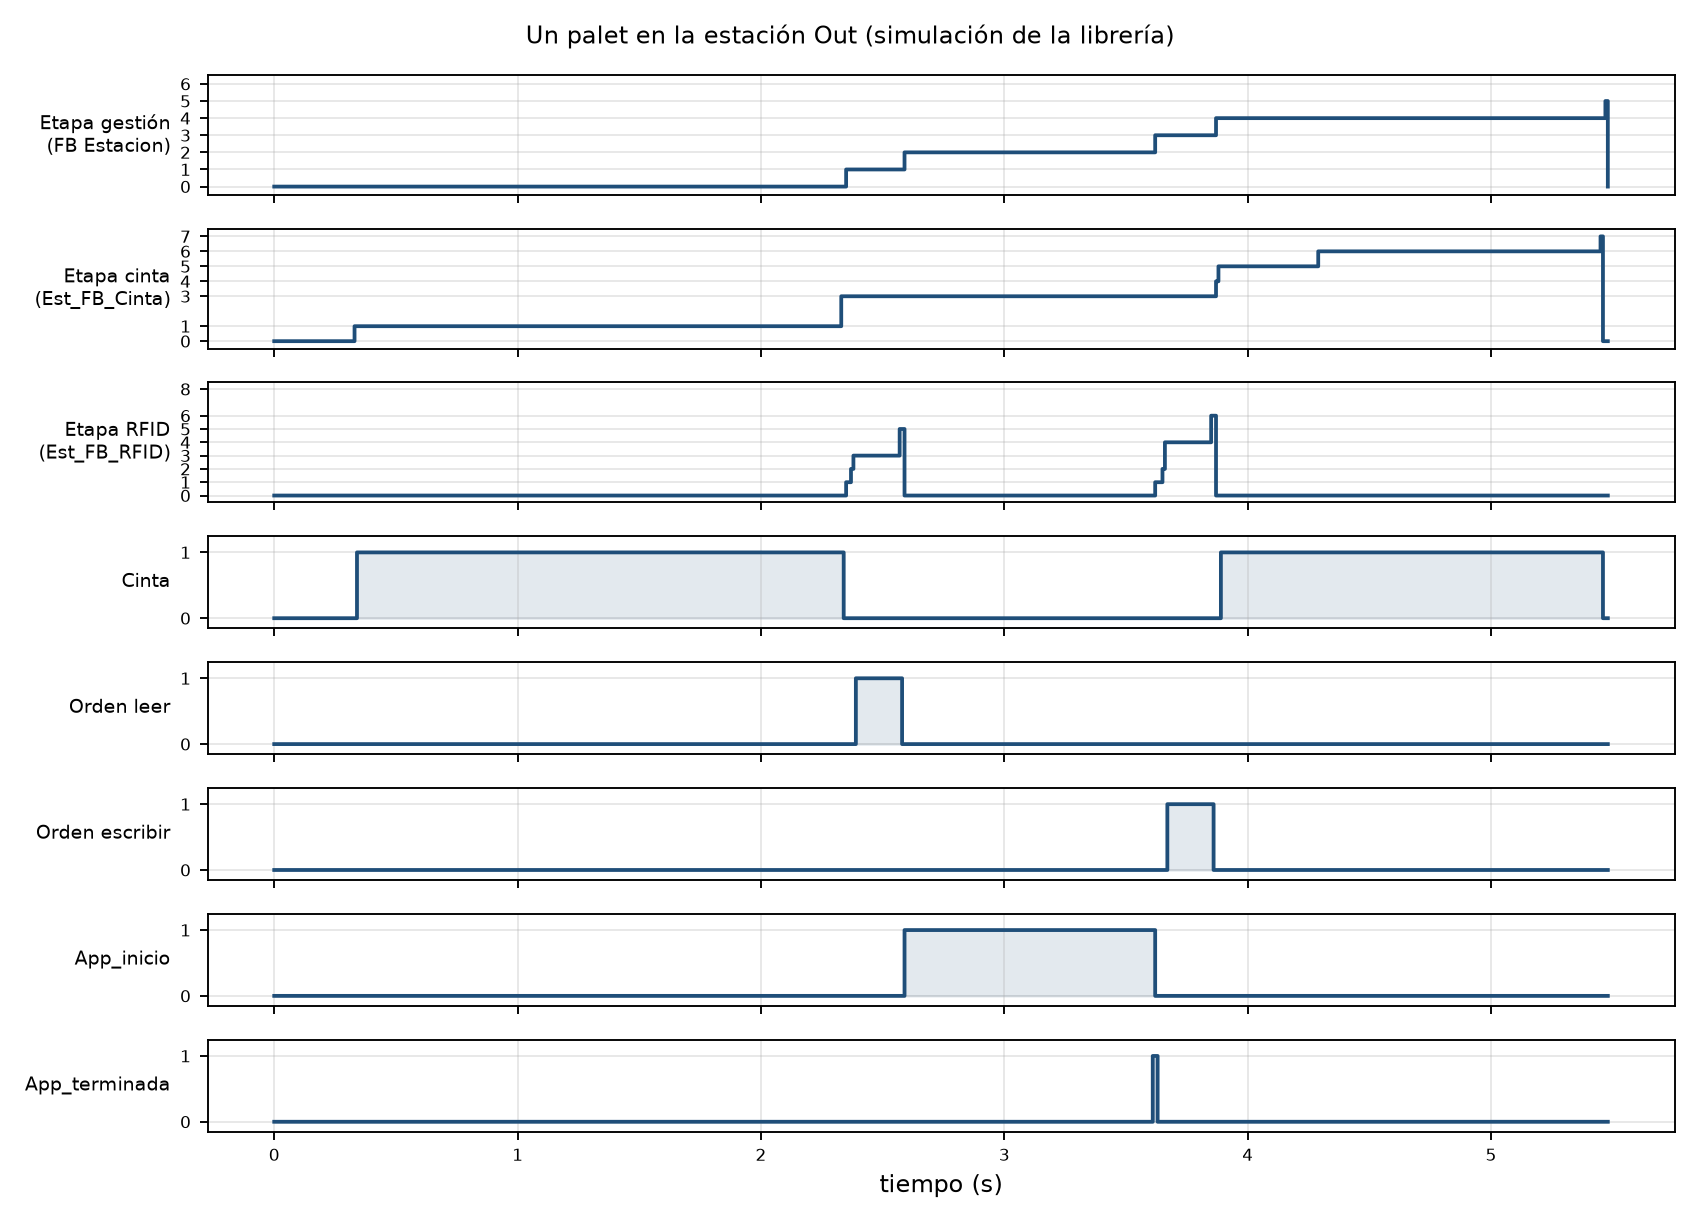
\includegraphics[width=\textwidth]{figuras/crono_ciclo_out.png}
\caption{Un palet en la estación Out (simulación).}
\end{figure}

\subsection{Qué \emph{no} cubre el simulador}
\begin{itemize}
\item \textbf{El hardware real}: tiempos de IO-Link, ruido, polaridad de cada sensor, señales que no están conectadas.
\item \textbf{El PROFINET}, la HMI y las comunicaciones con otros PLC (cámara, Festo).
\item \textbf{Varios palets pegados} en la cinta (en la estación Out se probó con el simulador de CIROS, no con este).
\item \textbf{Tu aplicación real.} Los ejemplos prueban el patrón, no tu mecanismo.
\end{itemize}

\section{Pruebas de aceptación en tu estación}
Después de migrar, haz estas pruebas en este orden. Cada una tiene una forma de hacerla y un resultado esperado. Usa una tabla de observación (\menu{Watch table}) con \cod{DB\_Estacion} y las etapas de \cod{Est\_DB\_Estacion} (\cod{Etapa\_gestion}, y las de las instancias de cinta y RFID).

\begin{center}
\small
\begin{longtable}{>{\bfseries}p{0.7cm}p{3.6cm}p{5.0cm}p{5.1cm}}
\toprule
N.º & Prueba & Cómo & Resultado esperado \\
\midrule\endhead
1 & Arranque sin palet & Alimenta, sin palets en la cinta. Observa \cod{App\_en\_reposo}. & \cod{App\_en\_reposo} verdadera; la luz de marcha se enciende (en automático). \\
2 & Marcha y paro & Pulsa marcha, luego paro. & Se enciende la luz de ciclo auto; el paro lo detiene. \\
3 & Entra un palet & Pon un palet en el extremo izquierdo de la cinta. & La cinta lo trae, se para en el tope; \cod{Palet\_en\_posicion}. \\
4 & Lectura del tag & Observa \cod{Imagen\_palet} cuando el palet esté parado. & Tus bytes aparecen con los valores del tag. Los demás, a cero. \\
5 & Tu aplicación & Observa \cod{App\_inicio}, \cod{App\_en\_reposo}, \cod{App\_terminada}. & \cod{App\_inicio} sube; tu mecanismo trabaja; al acabar sube \cod{App\_terminada} y se mantiene. \\
6 & Escritura del tag & Pasa el palet por una estación siguiente, o vuelve a leerlo. & Tus bytes han cambiado como esperabas; los demás, no. \\
7 & Evacuación & Observa la cinta. & El palet sale, el stopper vuelve a subir, la estación espera otro. \\
8 & Dos palets seguidos & Mete otro palet detrás. & El segundo se detiene y se procesa tras el primero. \\
9 & Emergencia en reposo & Pulsa la seta con la estación parada. & Luz de emergencia; la cinta no se mueve. \\
10 & Emergencia con tu aplicación trabajando & Pulsa la seta a mitad de tu secuencia. & Tus actuadores se paran; no se escribe el tag. Suelta la seta y pulsa rearme: se normaliza. \\
11 & Fallo del lector & Retira el tag o tapa la antena justo al llegar un palet. & A los 5\,s, etapa 6 (fallo RFID); luz de rearme. Con rearme, el palet sale sin procesar. \\
12 & Palet sin datos & Usa un palet con el tag a cero. & Tu estación se comporta según el valor «si vale 0» del mapa. \\
\bottomrule
\end{longtable}
\end{center}

\section{La primera vez en la maqueta real}\label{sec:primera-vez}
Es la primera vez que la librería habla con un lector y un stopper reales. Para hacerlo sin riesgo para el tag de los demás ni para la maqueta:

\reiniciapaso
\paso{Empieza con la escritura desactivada}
Pon \cod{Mascara\_escritura} a \cod{16\#00000000} en \cod{Main}. Con eso, la estación lee el tag pero escribe de vuelta \emph{exactamente lo que leyó}: no cambia nada. Es la prueba más segura.

\paso{Usa un palet de pruebas}
No uses un palet con datos de otro grupo. Si hace falta, escribe antes en su tag unos datos de ejemplo (por ejemplo los de la columna «Ejemplo» del Excel).

\paso{Prueba sin actuadores peligrosos}
Con tu mecanismo despejado, y la mano cerca de la seta. Observa las etapas en la tabla de observación en vez de ir a ciegas.

\paso{Comprueba la polaridad de los sensores}
En la tabla de observación de \cod{Entradas\_Basico} y \cod{Entradas\_Stopper}, con la maqueta parada: \cod{Boton\_paro} y \cod{Seta\_emergencia} deben estar a verdadero (son de contacto cerrado); \cod{Sensor\_stopper\_abajo} debe estar a falso con el stopper arriba. Si algo está al revés, no sigas: puede ser un cableado distinto del de la documentación.

\paso{Pasa un palet}
Pulsa marcha y mete un palet. Mira el recorrido de las etapas con la figura~\ref{fig:crono} al lado.

\paso{Activa la escritura}
Cuando la lectura y tu aplicación funcionen, pon tu \cod{Mascara\_escritura} real y repite con un palet de pruebas. Comprueba en el tag, con otra lectura, que cambiaron \textbf{solo tus bytes}.

\begin{ojo}
Si alguna vez ves que la estación se queda en la etapa 4 de la cinta (liberar) o que el palet no sale, revisa la polaridad del sensor \cod{Sensor\_stopper\_abajo} (apéndice~\ref{ap:abiertos}). Es la parte de la librería que más depende del cableado real.
\end{ojo}

\section{Lista completa de comprobaciones del simulador}
\small
\begin{longtable}{r p{12.2cm} c}
\toprule
\textbf{N.º} & \textbf{Comprobación} & \textbf{Resultado} \\
\midrule
\endhead
\multicolumn{3}{l}{\sffamily\bfseries\color{azul} Librería}\\
1 & Camara: el palet completa el ciclo y sale & \textcolor{verde}{\ding{51}} \\
2 & Camara: la app solo ve los bytes de Mascara\_lectura & \textcolor{verde}{\ding{51}} \\
3 & Camara: el tag queda como esperado & \textcolor{verde}{\ding{51}} \\
4 & Camara: los bytes ajenos (fuera de Mascara\_escritura) no cambian & \textcolor{verde}{\ding{51}} \\
5 & Camara: una sola escritura al tag por palet & \textcolor{verde}{\ding{51}} \\
6 & BackCover: el palet completa el ciclo y sale & \textcolor{verde}{\ding{51}} \\
7 & BackCover: la app solo ve los bytes de Mascara\_lectura & \textcolor{verde}{\ding{51}} \\
8 & BackCover: el tag queda como esperado & \textcolor{verde}{\ding{51}} \\
9 & BackCover: los bytes ajenos (fuera de Mascara\_escritura) no cambian & \textcolor{verde}{\ding{51}} \\
10 & BackCover: una sola escritura al tag por palet & \textcolor{verde}{\ding{51}} \\
11 & Press: el palet completa el ciclo y sale & \textcolor{verde}{\ding{51}} \\
12 & Press: la app solo ve los bytes de Mascara\_lectura & \textcolor{verde}{\ding{51}} \\
13 & Press: el tag queda como esperado & \textcolor{verde}{\ding{51}} \\
14 & Press: los bytes ajenos (fuera de Mascara\_escritura) no cambian & \textcolor{verde}{\ding{51}} \\
15 & Press: una sola escritura al tag por palet & \textcolor{verde}{\ding{51}} \\
16 & Out: el palet completa el ciclo y sale & \textcolor{verde}{\ding{51}} \\
17 & Out: la app solo ve los bytes de Mascara\_lectura & \textcolor{verde}{\ding{51}} \\
18 & Out: el tag queda como esperado & \textcolor{verde}{\ding{51}} \\
19 & Out: los bytes ajenos (fuera de Mascara\_escritura) no cambian & \textcolor{verde}{\ding{51}} \\
20 & Out: una sola escritura al tag por palet & \textcolor{verde}{\ding{51}} \\
21 & plantilla: el palet entra, se procesa y sale con la plantilla tal cual & \textcolor{verde}{\ding{51}} \\
22 & error RFID: la gestion pasa a "fallo RFID" (etapa 6) & \textcolor{verde}{\ding{51}} \\
23 & error RFID: la app no llega a arrancar & \textcolor{verde}{\ding{51}} \\
24 & error RFID: tras rearmar el palet se evacua & \textcolor{verde}{\ding{51}} \\
25 & error RFID: no se escribe nada en el tag & \textcolor{verde}{\ding{51}} \\
26 & emergencia: la app esta trabajando & \textcolor{verde}{\ding{51}} \\
27 & emergencia: Emergencia activa y la gestion vuelve a 0 & \textcolor{verde}{\ding{51}} \\
28 & emergencia: la cinta y el stopper se paran & \textcolor{verde}{\ding{51}} \\
29 & emergencia: no se escribe nada en el tag & \textcolor{verde}{\ding{51}} \\
30 & emergencia: tras soltar la seta y rearmar, Emergencia vuelve a 0 & \textcolor{verde}{\ding{51}} \\
\multicolumn{3}{l}{\sffamily\bfseries\color{azul} Ejemplos de aplicación}\\
31 & Press: completa el ciclo & \textcolor{verde}{\ding{51}} \\
32 & Press: golpes realizados = 2 (byte 16) & \textcolor{verde}{\ding{51}} \\
33 & Press: bit 2 de "completadas" puesto (byte 4 = 7) & \textcolor{verde}{\ding{51}} \\
34 & Press: el resto del bloque intacto & \textcolor{verde}{\ding{51}} \\
35 & Press: sin tapa trasera en el tag no prensa ni marca completada & \textcolor{verde}{\ding{51}} \\
36 & Press: si no esta en "estaciones a realizar", el palet pasa sin cambios & \textcolor{verde}{\ding{51}} \\
37 & BackCover: completa el ciclo & \textcolor{verde}{\ding{51}} \\
38 & BackCover: estado = requerida + colocada (byte 12 = 3) & \textcolor{verde}{\ding{51}} \\
39 & BackCover: bit 1 de "completadas" (byte 4 = 3) & \textcolor{verde}{\ding{51}} \\
40 & BackCover: el resto del bloque intacto & \textcolor{verde}{\ding{51}} \\
41 & BackCover: sin stock -> byte 12 = requerida + falta stock (5) y sin bit de completada & \textcolor{verde}{\ding{51}} \\
42 & Camara: completa el ciclo con el tag vacio & \textcolor{verde}{\ding{51}} \\
43 & Camara: inicializa el bloque (byte 0 = A5) & \textcolor{verde}{\ding{51}} \\
44 & Camara: usa el job por defecto (4) sin datos & \textcolor{verde}{\ding{51}} \\
45 & Camara: calidad OK (5=1), resultado (9=7), ImageID (10=42), intentos (11=1), completada (4=1) & \textcolor{verde}{\ding{51}} \\
46 & Camara: job deducido de los fusibles (byte 20 = 2 -> job 3) & \textcolor{verde}{\ding{51}} \\
47 & Camara: NOK -> calidad 2 y rechazo 16\#11 & \textcolor{verde}{\ding{51}} \\
48 & Camara: los bytes que no escribe (8, 20) no cambian & \textcolor{verde}{\ding{51}} \\
\bottomrule
\end{longtable}

\normalsize

\chapter{Problemas frecuentes}\label{cap:problemas}

Una tabla de síntomas, causas probables y soluciones. Los mensajes de compilación son los que TIA muestra de verdad (en inglés, como en la VM del grupo); varios se han visto durante la preparación de la librería.

\section{Al compilar}
\begin{center}
\small
\begin{longtable}{>{\raggedright\arraybackslash}p{4.4cm}>{\raggedright\arraybackslash}p{4.7cm}>{\raggedright\arraybackslash}p{5.2cm}}
\toprule
\textbf{Mensaje} & \textbf{Causa} & \textbf{Solución} \\
\midrule\endhead
\cod{Tag "Entradas\_Basico" not defined} (y los otros seis) & No has copiado la tabla de variables de la librería. & Copia \menu{Tabla de variables estándar} de la plantilla, o crea los siete tags (sección~\ref{sec:tags}). \\
\cod{Type conflict for "Entradas\_APP"}, \cod{Block call was invalid because interface was changed in the meantime} & Una llamada en \cod{Main} se hizo con una versión anterior de un bloque y su interfaz ha cambiado. & Borra la caja del bloque en la red y arrástralo otra vez desde el árbol. Cablea los pines de nuevo. \\
\cod{The operand required at the input or output is missing or has an incorrect data type} & Un pin obligatorio sin cablear (los \texttt{in/out}: \cod{OutBasico}, \cod{OutRFID}, \cod{Imagen\_palet}) o con un tipo equivocado. & Haz doble clic en el mensaje: TIA te lleva a la red y marca el pin en rojo. \\
\cod{Inputs or outputs are used that do not exist in the configured hardware} (aviso) & Algún tag apunta a una dirección que no tiene módulo en tu configuración. & Es normal al principio. Ajusta la dirección del tag o la configuración de dispositivos. \\
\cod{The sign or the accuracy of the value may be lost} (aviso, en \cod{Est\_FB\_RFID}) & Conversión implícita entre tipos de entero (no afecta al funcionamiento). & Inofensivo. No lo toques. \\
No me deja editar un bloque de la librería & Es lo normal: está ligado a la librería. & Si necesitas un cambio, ve al capítulo~\ref{cap:mantenimiento}. \\
Errores en tu código antiguo (nombres que no existen) & Usa variables o bloques que la librería sustituye. & Muévelo a la carpeta \menu{Antiguo} (fase 3). \\
\bottomrule
\end{longtable}
\end{center}

\section{Al ejecutar}
\begin{center}
\small
\begin{longtable}{>{\raggedright\arraybackslash}p{4.2cm}>{\raggedright\arraybackslash}p{5.0cm}>{\raggedright\arraybackslash}p{5.1cm}}
\toprule
\textbf{Síntoma} & \textbf{Causa probable} & \textbf{Qué mirar o hacer} \\
\midrule\endhead
La estación no arranca (la luz de marcha no se enciende) & No se cumplen las condiciones iniciales. & Mira \cod{Estacion\_cond\_iniciales} en la instancia: \cod{App\_en\_reposo} falso, stopper bajado, error de RFID pendiente, o emergencia. \\
La cinta no se mueve & \cod{Inhibir\_cinta} verdadera; el ciclo no está activo; o estás con la versión 1.0.0. & Mira \cod{Inhibir\_cinta} y \cod{Cinta\_habilitada}. Comprueba la versión de la librería (debe ser $\geq$ \vlib). \\
El palet no se detiene en el tope & \cod{Sensor\_ind\_bien\_pos} no llega o con polaridad invertida. & Observa \cod{Entradas\_Basico.Sensor\_ind\_bien\_pos} con el palet en el tope. \\
Se queda en la etapa 1 de la secuencia (leer) y salta a fallo & Lector sin tag detectado, antena apagada, o el módulo IO-Link no está en modo «Scan user data». & Mira \cod{Tag\_detectado}, \cod{Tag\_antena\_apagada}, \cod{Tag\_error}. Comprueba la configuración del lector. A los 5\,s la etapa 6 es lo previsto. \\
La lectura funciona pero \cod{Imagen\_palet} está a cero & Tu \cod{Mascara\_lectura} no incluye esos bytes (o es 0). & Revisa las máscaras (sección~\ref{sec:calculo-mascara}). \\
Tus bytes del tag han cambiado, pero uno aparece a cero & Escribes un byte que no está en tu lectura (regla O1). & Añade ese byte a \cod{Mascara\_lectura}. \\
No cambia nada en el tag & \cod{Mascara\_escritura} a cero (es el valor por defecto) o sin los bits de tus bytes. & Pon tu máscara de escritura. \\
Los bytes de otras estaciones se estropean & Escribes bytes que no son tuyos, o las direcciones de lectura y escritura son distintas. & Reglas O2 y O5 (sección~\ref{sec:reglas-oro}). \\
El palet se procesa dos veces & Tu aplicación vuelve a reposo mientras \cod{App\_inicio} sigue activa (regla R3), o las llamadas en \cod{Main} están en otro orden. & Mira el estado de fin de la plantilla y el orden de las dos redes de \cod{Main}. \\
La estación se queda esperando en la etapa 2 & Tu aplicación no sube \cod{App\_terminada}. & Observa los estados de tu aplicación; añade un temporizador de seguridad y \cod{App\_alarma}. \\
Tras la emergencia, el rearme no la quita & La seta sigue pulsada. & Se necesita soltar la seta \emph{y} un flanco de rearme. \\
La luz de rearme está encendida y no sé por qué & Tres causas posibles: emergencia, fallo del RFID (etapa 6), o tu \cod{App\_rearme\_requerido}. & Mira las tres señales. \\
\bottomrule
\end{longtable}
\end{center}

\section{Si nada de esto sirve}
Antes de pedir ayuda, reúne:
\begin{enumerate}
\item la versión de la librería (en el panel de librerías, columna \menu{Version});
\item una captura de la tabla de observación con las etapas de \cod{Est\_DB\_Estacion};
\item los valores de tus máscaras y de \cod{Direccion\_lectura};
\item el mensaje de error completo, si hay.
\end{enumerate}
Con eso casi siempre se encuentra el problema en pocos minutos.

\chapter{Mantener y cambiar la librería}\label{cap:mantenimiento}

Una librería compartida solo funciona si los cambios se hacen con orden. Este capítulo explica cómo se cambia y cómo se reparte una versión nueva.

\section{Cuándo cambiar la librería (y cuándo no)}
\begin{itemize}
\item \textbf{Sí}: hay un fallo; hay una necesidad que comparten varias estaciones.
\item \textbf{No}: algo que solo necesita tu estación (va en tu aplicación); un cambio de significado de un byte del tag (va en el Excel y en tus constantes).
\end{itemize}

\section{Cómo se pide un cambio}
Se manda al grupo (y a quien mantiene la librería): qué ocurre, en qué estación y con qué versión, y qué propones. Si es un fallo, el material del capítulo~\ref{cap:problemas}, «si nada de esto sirve». No se corrige en el proyecto de cada uno: no se puede, y si se pudiera, las estaciones dejarían de ser iguales.

\section{Cómo se hace un cambio}
Lo hace una sola persona, en la librería:

\reiniciapaso
\paso{Edita el tipo en la librería}
En el panel de librerías, abre el tipo (por ejemplo, \cod{Est\_FB\_Estacion}) para editarlo. La librería exige que se edite el \emph{tipo}, no la copia que hay en un proyecto.

\paso{Prueba el cambio}
Compila. Después, ejecuta las pruebas del simulador de la librería (capítulo~\ref{cap:pruebas}) si las tienes, o las de aceptación del grupo.

\paso{Asigna una versión nueva}
Con \menu{Assign version} (Asignar versión) sobre el tipo, dale un número nuevo. La versión de un tipo ya asignada no se puede modificar: cualquier arreglo es una versión nueva.

\paso{Archiva la librería}
En el panel de librerías, clic derecho sobre \menu{CPLabCore} y \menu{Archive library...} (Archivar librería). Elige el formato comprimido (\texttt{.zal20}) y el nombre con la versión: \texttt{CPLabCore\_v1.0.2.zal20}.

\begin{figure}[ht]
\centering
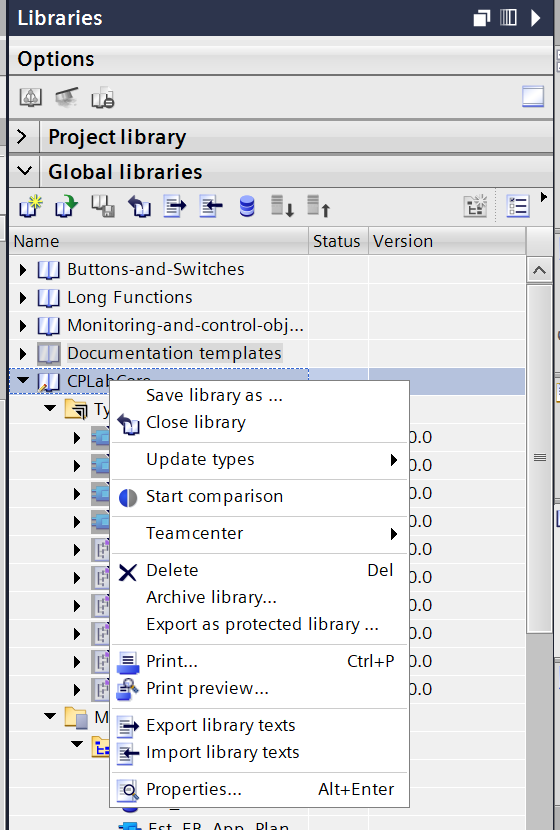
\includegraphics[width=0.55\textwidth]{capturas/menu_biblioteca.png}
\caption{El menú de la librería: \menu{Archive library...}, \menu{Update types}, \menu{Save library as...} y otros.}
\end{figure}

\paso{Avisa al grupo}
Con el nuevo archivo, qué cambia, y si hace falta cambiar algo en \cod{Main} o en las aplicaciones.

\section{Numeración de versiones}
\begin{center}
\small
\begin{tabularx}{\textwidth}{>{\bfseries}p{2.8cm}p{2.8cm}X}
\toprule
Cambio & Se incrementa & Ejemplo \\
\midrule
Arreglo de un fallo, sin cambiar pines & el último número & 1.0.1 $\rightarrow$ 1.0.2 \\
Función nueva compatible (pines nuevos con valor por defecto) & el segundo & 1.0.2 $\rightarrow$ 1.1.0 \\
Cambio incompatible (pines quitados, otro formato) & el primero & 1.1.0 $\rightarrow$ 2.0.0 \\
\bottomrule
\end{tabularx}
\end{center}
Una versión de «arreglo» se puede actualizar sin pensar; una «compatible» también, pero no hace falta usar lo nuevo; una «incompatible» exige revisar \cod{Main} y las aplicaciones.

\section{Registro de cambios}
\begin{center}
\small
\begin{tabularx}{\textwidth}{>{\bfseries}p{1.6cm}p{2.7cm}X}
\toprule
Versión & Fecha & Cambios \\
\midrule
1.0.1 & 12/11/2026 & Corrige un error en \cod{Est\_FB\_Estacion}: la condición que apaga la cinta estaba invertida (\cod{IF NOT Inhibir\_cinta} pasa a \cod{IF Inhibir\_cinta}) y la cinta no arrancaba nunca. \\
1.0.0 & 12/11/2026 & Primera versión: \cod{Est\_FB\_Estacion}, \cod{Est\_FB\_Modo}, \cod{Est\_FB\_Cinta}, \cod{Est\_FB\_RFID} y los seis UDT, con la imagen de 28 bytes, las máscaras y las direcciones. \textbf{No usar: error de la cinta.} \\
\bottomrule
\end{tabularx}
\end{center}

\section{Mejoras que se pueden plantear}
Cosas que se han visto al hacer la librería y que mejorarían una versión futura (el apéndice~\ref{ap:abiertos} las detalla):
\begin{itemize}
\item Que la librería lea siempre la unión de la máscara de lectura y la de escritura, para eliminar la regla de oro O1.
\item Un tiempo máximo para la aplicación, con aviso, para que una aplicación atascada no bloquee la estación.
\item Quitar la etapa de la cinta que no se usa.
\item Revisar con el hardware real la polaridad del sensor del stopper.
\end{itemize}

\appendix
\chapter{Hoja de referencia rápida}\label{ap:referencia}
Una página para tener a mano cuando ya conoces la librería.

\section*{Lo que cambia en cada estación}
\begin{center}
\small
\begin{tabularx}{\textwidth}{>{\ttfamily}p{4.2cm}X}
\toprule
\textnormal{\textbf{Qué}} & \textbf{Dónde} \\
\midrule
Mascara\_lectura, Mascara\_escritura & En la llamada a \cod{Est\_FB\_Estacion} de \cod{Main} (capítulo~\ref{cap:mapa}). \\
Direccion\_lectura, Direccion\_escritura & Igual, las dos iguales (por defecto \cod{16\#0000}). \\
Tu aplicación & Un bloque tuyo, copia de \cod{Est\_FB\_App\_Plantilla}. \\
Tus constantes \cod{IDX\_*} & Dentro de tu aplicación. \\
\bottomrule
\end{tabularx}
\end{center}

\section*{El contrato (desde tu aplicación)}
\begin{center}
\small
\begin{tabular}{>{\ttfamily}l l >{\ttfamily}l l}
\toprule
\textnormal{\textbf{Recibes}} & & \textnormal{\textbf{Entregas}} & \\
\midrule
App\_inicio & empieza & App\_en\_reposo & lista para un palet \\
Emergencia & hay emergencia & App\_terminada & acabé; resultado en la imagen \\
Rearme & pulso de rearme & App\_alarma & parpadeo Q2 (opcional) \\
Imagen\_palet & 28 bytes & App\_rearme\_requerido & luz de rearme (opcional) \\
 & & Inhibir\_cinta & la cinta no se mueve \\
\bottomrule
\end{tabular}
\end{center}

\section*{Las siete reglas de la aplicación}
R1 Declara tu reposo.\quad R2 Empieza solo con \cod{App\_inicio} y en reposo.\quad R3 Termina con \cod{App\_terminada} y mantenla hasta que \cod{App\_inicio} baje.\quad R4 El resultado, en la imagen, antes de terminar.\quad R5 Toca solo tus bytes.\quad R6 Obedece la emergencia.\quad R7 No esperes un límite de tiempo: ponlo tú.

\section*{Las reglas de oro de las máscaras}
O1 Todo byte que escribes, también lo lees.\quad O2 Escribe solo tus bytes.\quad O3 Las banderas, con OR.\quad O4 Un 0 significa «sin dato».\quad O5 La misma dirección para leer y escribir.\quad O6 Los bytes 20 a 27, solo si se ha acordado.\quad O7 Los números de dos bytes, juntos.

\section*{Calcular una máscara}
Para cada byte $n$ de la lista, súmale $2^{n}$ \,(byte 0 = 1, byte 1 = 2, byte 2 = 4, byte 3 = 8, byte 4 = \cod{10}, byte 5 = \cod{20}\dots). En hexadecimal: cada grupo de cuatro bytes es un dígito, con valores 1, 2, 4 y 8.

\begin{center}
\footnotesize\setlength{\tabcolsep}{2.0pt}
\begin{tabular}{l|cccc|cccc|cccc|cccc|cccc|cccc|cccc}
Dígito & \multicolumn{4}{c|}{1.º} & \multicolumn{4}{c|}{2.º} & \multicolumn{4}{c|}{3.º} & \multicolumn{4}{c|}{4.º} & \multicolumn{4}{c|}{5.º} & \multicolumn{4}{c|}{6.º} & \multicolumn{4}{c}{7.º} \\
Bytes & 0&1&2&3 & 4&5&6&7 & 8&9&10&11 & 12&13&14&15 & 16&17&18&19 & 20&21&22&23 & 24&25&26&27 \\
Valor & 1&2&4&8 & 1&2&4&8 & 1&2&4&8 & 1&2&4&8 & 1&2&4&8 & 1&2&4&8 & 1&2&4&8 \\
\end{tabular}
\end{center}

\section*{Las máscaras del grupo}
\begin{tabularx}{\textwidth}{>{\bfseries}l p{3.1cm} c c X}
\toprule
Estación & Bytes que usa & \texttt{Mascara\_lectura} & \texttt{Mascara\_escritura} & Qué escribe \\
\midrule
Cámara & 0, 1, 2, 3, 4, 5, 6, 8, 9, 10, 11, 20 & \texttt{16\#00100F7F} & \texttt{16\#00000E7F} & bytes 0 a 6 (los 0 a 3 solo si el tag está vacío), 9, 10 y 11 \\
BackCover & 3, 4, 12, 23 & \texttt{16\#00801018} & \texttt{16\#00001010} & byte 4 (bit 1) y byte 12 \\
Press & 3, 4, 12, 13, 14, 15, 16 & \texttt{16\#0001F018} & \texttt{16\#00010010} & byte 4 (bit 2) y byte 16 \\
Out & 5, 9, 17, 21, 22 & \texttt{16\#00620220} & \texttt{16\#0FFFFFFF} & los 28 bytes: deja el bloque a cero \\
\bottomrule
\end{tabularx}


\section*{Las siete tags}
\cod{Entradas\_APP} \cod{\%I0.0}, \cod{Entradas\_Basico} \cod{\%I1.0}, \cod{Entradas\_RFID} \cod{\%I10.0}, \cod{Entradas\_Stopper} \cod{\%I42.0}, \cod{Salidas\_APP} \cod{\%Q0.0}, \cod{Salidas\_Basico} \cod{\%Q1.0}, \cod{Salidas\_RFID} \cod{\%Q10.0}.

\chapter{Direcciones y UDT}\label{ap:direcciones}

\section{Los módulos de la estación}
Según el manual de la CP-Lab (apartado 11.2.1) y la configuración de la estación Out, estas direcciones son iguales en todas las estaciones:

\begin{center}
\small
\begin{tabularx}{\textwidth}{>{\bfseries}p{4.3cm}p{2.7cm}X}
\toprule
Parte de la máquina & Entradas / Salidas & Contenido \\
\midrule
Aplicación (1 byte) & \cod{\%E0} / \cod{\%A0} & Señales propias de cada estación (cambia de una a otra). \\
Módulo básico & \cod{\%E1} / \cod{\%A1} & Botonera, selector, seta, sensores de cinta; luces, cinta, stopper. \\
Lector RFID (IO-Link) & \cod{\%E10} / \cod{\%A10} & Estado, error, dirección y 28 bytes de datos. \\
Módulo del stopper (IO-Link) & \cod{\%E42} & Sensores inductivos, encoder, «stopper abajo». \\
\bottomrule
\end{tabularx}
\end{center}

\section{Los UDT bit a bit}
\subsection*{\texttt{UDT\_Entradas\_Basico}}
Tag \texttt{Entradas\_Basico}, desde \texttt{\%I1.0}.\par\smallskip
\begin{tabular}{>{\ttfamily\small}p{5.2cm}>{\ttfamily\small}p{4.2cm}>{\ttfamily\small}p{2.4cm}}
\toprule
\textnormal{\textbf{Miembro}} & \textnormal{\textbf{Tipo}} & \textnormal{\textbf{Dirección}} \\
\midrule
Boton\_marcha & Bool & \%I1.0 \\
Boton\_paro & Bool & \%I1.1 \\
Selector\_modo & Bool & \%I1.2 \\
Boton\_rearme & Bool & \%I1.3 \\
Sensor\_ind\_bien\_pos & Bool & \%I1.4 \\
Seta\_emergencia & Bool & \%I1.5 \\
Sensor\_palet\_izq & Bool & \%I1.6 \\
Sensor\_palet\_dch & Bool & \%I1.7 \\
\bottomrule
\end{tabular}

\medskip
\subsection*{\texttt{UDT\_Salidas\_Basico}}
Tag \texttt{Salidas\_Basico}, desde \texttt{\%Q1.0}.\par\smallskip
\begin{tabular}{>{\ttfamily\small}p{5.2cm}>{\ttfamily\small}p{4.2cm}>{\ttfamily\small}p{2.4cm}}
\toprule
\textnormal{\textbf{Miembro}} & \textnormal{\textbf{Tipo}} & \textnormal{\textbf{Dirección}} \\
\midrule
Led\_boton\_marcha & Bool & \%Q1.0 \\
Led\_boton\_rearme & Bool & \%Q1.1 \\
Led\_q1\_ciclo\_auto & Bool & \%Q1.2 \\
Led\_q2\_emergencia & Bool & \%Q1.3 \\
Cinta\_dch & Bool & \%Q1.4 \\
Cinta\_izq & Bool & \%Q1.5 \\
Cinta\_velocidad\_baja & Bool & \%Q1.6 \\
Bajar\_stopper & Bool & \%Q1.7 \\
\bottomrule
\end{tabular}

\medskip
\subsection*{\texttt{UDT\_Entradas\_Stopper}}
Tag \texttt{Entradas\_Stopper}, desde \texttt{\%I42.0}.\par\smallskip
\begin{tabular}{>{\ttfamily\small}p{5.2cm}>{\ttfamily\small}p{4.2cm}>{\ttfamily\small}p{2.4cm}}
\toprule
\textnormal{\textbf{Miembro}} & \textnormal{\textbf{Tipo}} & \textnormal{\textbf{Dirección}} \\
\midrule
Sensor\_ind\_0 & Bool & \%I42.0 \\
Sensor\_ind\_1 & Bool & \%I42.1 \\
Sensor\_ind\_2 & Bool & \%I42.2 \\
Sensor\_ind\_3 & Bool & \%I42.3 \\
Reservado\_E2\_4 & Bool & \%I42.4 \\
Reservado\_E2\_5 & Bool & \%I42.5 \\
Reservado\_E2\_6 & Bool & \%I42.6 \\
Sensor\_stopper\_abajo & Bool & \%I42.7 \\
\bottomrule
\end{tabular}

\medskip
\subsection*{\texttt{UDT\_Entradas\_RFID}}
Tag \texttt{Entradas\_RFID}, desde \texttt{\%I10.0}.\par\smallskip
\begin{tabular}{>{\ttfamily\small}p{5.2cm}>{\ttfamily\small}p{4.2cm}>{\ttfamily\small}p{2.4cm}}
\toprule
\textnormal{\textbf{Miembro}} & \textnormal{\textbf{Tipo}} & \textnormal{\textbf{Dirección}} \\
\midrule
Tag\_datos\_escritos & Bool & \%I10.0 \\
Tag\_datos\_leidos & Bool & \%I10.1 \\
Reservado\_E4\_2 & Bool & \%I10.2 \\
Reservado\_E4\_3 & Bool & \%I10.3 \\
Tag\_antena\_apagada & Bool & \%I10.4 \\
Tag\_detectado & Bool & \%I10.5 \\
Tag\_error & Bool & \%I10.6 \\
Tag\_proceso\_listo & Bool & \%I10.7 \\
Tag\_codigo\_error & Byte & \%IB11 \\
Tag\_direccion\_confirmada & Word & \%IW12 \\
Tag\_datos\_leidos\_escritos & Array[0..27] of Byte & \%I14.0 ... \%I41.7 \\
\bottomrule
\end{tabular}

\medskip
\subsection*{\texttt{UDT\_Salidas\_RFID}}
Tag \texttt{Salidas\_RFID}, desde \texttt{\%Q10.0}.\par\smallskip
\begin{tabular}{>{\ttfamily\small}p{5.2cm}>{\ttfamily\small}p{4.2cm}>{\ttfamily\small}p{2.4cm}}
\toprule
\textnormal{\textbf{Miembro}} & \textnormal{\textbf{Tipo}} & \textnormal{\textbf{Dirección}} \\
\midrule
Tag\_escribir & Bool & \%Q10.0 \\
Tag\_leer & Bool & \%Q10.1 \\
Tag\_reservado\_2 & Bool & \%Q10.2 \\
Tag\_reservado\_3 & Bool & \%Q10.3 \\
Tag\_antena\_apagar & Bool & \%Q10.4 \\
Tag\_reservado\_5 & Bool & \%Q10.5 \\
Tag\_reservado\_6 & Bool & \%Q10.6 \\
Tag\_reservado\_7 & Bool & \%Q10.7 \\
Reservado\_AB5 & Byte & \%QB11 \\
Tag\_direccion\_leer\_escribir & Word & \%QW12 \\
Tag\_datos\_a\_escribir & Array[0..27] of Byte & \%Q14.0 ... \%Q41.7 \\
\bottomrule
\end{tabular}

\medskip


\begin{ojo}
Estos UDT tienen que estar \textbf{bit a bit} como se muestran. Un miembro movido de sitio cambia el sensor al que se refiere. Por eso los tipos de la librería no se editan en los proyectos.
\end{ojo}

\chapter{Listados de código}\label{ap:listados}

El código SCL completo de la librería y de los ejemplos, tal cual está en los archivos. Se incluye para que se pueda leer sin abrir TIA. Los acentos se han quitado de los comentarios para poder imprimirlos.

\section{Bloques de la librería (versión \vlib)}
\listado{Est_FB_Estacion}{Est\_FB\_Estacion: la secuencia del palet}
\listado{Est_FB_Modo}{Est\_FB\_Modo: modos y emergencia}
\listado{Est_FB_Cinta}{Est\_FB\_Cinta: cinta y stopper}
\listado{Est_FB_RFID}{Est\_FB\_RFID: lector RFID, imagen y máscaras}

\section{Plantilla de aplicación}
\listado{Est_FB_App_Plantilla}{Est\_FB\_App\_Plantilla}

\section{Ejemplos de aplicación}
\listado{FB_App_Press_Ejemplo}{FB\_App\_Press\_Ejemplo}
\listado{FB_App_BackCover_Ejemplo}{FB\_App\_BackCover\_Ejemplo}
\listado{FB_App_Camara_Ejemplo}{FB\_App\_Camara\_Ejemplo}

\section{Aplicación completa de la estación Out}
\listado{FB_App_Out}{FB\_App\_Out: la aplicación de la estación Out (como ejemplo de una aplicación completa)}

\chapter{Hojas para imprimir}\label{ap:checklists}

\section{Inventario de tu estación}
\begin{center}
\renewcommand{\arraystretch}{1.5}
\begin{tabularx}{\textwidth}{|>{\bfseries}p{3.6cm}|X|}
\hline
Estación & \\ \hline
Quién migra & \\ \hline
Fecha & \\ \hline
\multicolumn{2}{|l|}{\textbf{1. Mis señales físicas} (sensores y actuadores de la aplicación; nombre y dirección)} \\ \hline
\multicolumn{2}{|p{15cm}|}{\vspace{2.6cm}} \\ \hline
\multicolumn{2}{|l|}{\textbf{2. Mis datos del palet} (byte del bloque, qué es, si lo leo, si lo escribo)} \\ \hline
\multicolumn{2}{|p{15cm}|}{\vspace{3.2cm}} \\ \hline
\multicolumn{2}{|l|}{\textbf{3. Cuándo puedo empezar} (condición de reposo)} \\ \hline
\multicolumn{2}{|p{15cm}|}{\vspace{1.6cm}} \\ \hline
\multicolumn{2}{|l|}{\textbf{4. Cuándo he terminado}} \\ \hline
\multicolumn{2}{|p{15cm}|}{\vspace{1.6cm}} \\ \hline
\multicolumn{2}{|l|}{\textbf{Mis máscaras}} \\ \hline
\cod{Mascara\_lectura} & 16\# \\ \hline
\cod{Mascara\_escritura} & 16\# \\ \hline
\end{tabularx}
\end{center}

\section{Lista de la migración}
\begin{itemize}[label=$\square$,itemsep=4pt]
\item Copia de seguridad hecha (nombre: \dotfill).
\item Inventario relleno.
\item Direcciones de hardware comprobadas.
\item Librería \vlib\ desarchivada.
\item \cod{Est\_FB\_Estacion} arrastrada (con sus tres FB y seis UDT).
\item Tabla de variables copiada o siete tags creados.
\item Código antiguo apartado en la carpeta \menu{Antiguo}.
\item Aplicación creada a partir de la plantilla.
\item Constantes \cod{IDX\_*} y máscaras calculadas.
\item \cod{Main}: red 1 (\cod{Est\_FB\_Estacion}) y red 2 (aplicación).
\item Compila con 0 errores.
\item Contrato comprobado (cinco comprobaciones del capítulo~\ref{cap:contrato}).
\item Pruebas de aceptación 1 a 12 hechas.
\item Primera vez en la maqueta con la escritura desactivada.
\item Escritura activada y bytes comprobados.
\end{itemize}

\section{Pruebas de aceptación}
\begin{center}
\renewcommand{\arraystretch}{1.5}
\begin{tabular}{|r|p{6.2cm}|c|p{4.8cm}|}
\hline
N.º & Prueba & OK & Observaciones \\ \hline
1 & Arranque sin palet & & \\ \hline
2 & Marcha y paro & & \\ \hline
3 & Entra un palet & & \\ \hline
4 & Lectura del tag & & \\ \hline
5 & Tu aplicación & & \\ \hline
6 & Escritura del tag & & \\ \hline
7 & Evacuación & & \\ \hline
8 & Dos palets seguidos & & \\ \hline
9 & Emergencia en reposo & & \\ \hline
10 & Emergencia con la aplicación trabajando & & \\ \hline
11 & Fallo del lector & & \\ \hline
12 & Palet sin datos & & \\ \hline
\end{tabular}
\end{center}

\chapter{Puntos abiertos y mejoras}\label{ap:abiertos}

Lo que no está cerrado, dicho con claridad. Ninguno impide usar la librería, pero conviene saberlo.

\section{Por comprobar en la maqueta real}
\begin{enumerate}
\item \textbf{Polaridad de \cod{Sensor\_stopper\_abajo}.} La etapa 4 de la cinta avanza cuando este sensor \emph{deja} de estar activo, y el simulador cumple esa condición al instante. El manual lo define como «stopper abajo». Hay que ver con la maqueta, con el stopper subido y bajado, qué valor da el sensor, y si la condición debe ser la contraria.
\item \textbf{Tamaño del bloque, 24 o 28 bytes.} El manual menciona «bloques de 24 bytes» en un apartado y 28 en el resto. La librería usa 28, como el UDT del lector y el Excel.
\item \textbf{Comportamiento del lector real} con tiempos reales (el simulador lo imita con 0,12\,s de proceso).
\item \textbf{Varios palets pegados.} Se comprobó con la estación Out en el simulador antiguo, no en el de la librería.
\end{enumerate}

\section{Por decidir en el grupo}
\begin{enumerate}
\item \textbf{Qué escribe Out exactamente.} El Excel dice que Out escribe el byte 4 (bit 3) y el 18, \emph{y además} pone todo el bloque a cero. Como el cero lo pisa todo, la librería está probada con la escritura completa a cero. Si se prefiere conservar los bytes 4 y 18, la máscara de Out sería \cod{16\#00040010} y no se borraría.
\item \textbf{Calidad «sin evaluar» (byte 5 igual a 0).} Out lo trata como NOK. El mapa no dice nada.
\item \textbf{Qué almacén recibe qué.} En el simulador antiguo la tapa buena iba al almacén derecho; el Excel dice «OK izquierdo, NOK derecho». La aplicación de Out del proyecto actual manda OK a la derecha. Hay que dejarlo escrito en el Excel.
\item \textbf{Job por defecto de la cámara} (en el ejemplo, el 4).
\item \textbf{Bytes 20 a 23}: propuesta de datos de otros grupos, aún sin acordar.
\end{enumerate}

\section{Mejoras para una versión futura}
\begin{enumerate}
\item Leer siempre la unión de la máscara de lectura y la de escritura, para que la regla O1 deje de existir.
\item Un temporizador máximo para la aplicación, con aviso.
\item Quitar la etapa 2 de la cinta, que no se alcanza.
\item Resolver los dos avisos de conversión de enteros de \cod{Est\_FB\_RFID}.
\item Añadir el prefijo \cod{Est\_} a los UDT, para que no choquen con tipos con el mismo nombre en el proyecto de cada uno.
\item Incluir el simulador de pruebas en la distribución de la librería.
\end{enumerate}

\section{Limitaciones de las comprobaciones}
\begin{itemize}
\item La copia de la \emph{tabla de variables} de la plantilla no se ha podido comprobar de manera automática, solo a mano en TIA.
\item Los ejemplos de aplicación compilan y se han probado con modelos físicos muy sencillos; los nombres de sus sensores y actuadores son de ejemplo.
\item El archivo \texttt{.zal20} de la versión 1.0.0 contiene el error de la cinta y no debe usarse.
\end{itemize}

\end{document}
